%==============================================================================
%  IITISoC 2026  |  Domain: DEIMoS
%  Attitude Control of a Satellite Using Reaction Wheels
%  END-EVALUATION REPORT  --  IEEE two-column format
%
%  Vivek Swamy (250003086)  |  Tulika Chowdhury (250003084)
%
%  Compile:  pdflatex DEIMoS_Final_Report.tex   (run 3x for TOC + crossrefs)
%  Requires: IEEEtran.cls
%
%  ---------------------------------------------------------------------------
%  RESTRUCTURED DRAFT -- what changed from the previous version
%  ---------------------------------------------------------------------------
%  Every number that could be measured from the code has been measured and
%  filled in.  \VAL{} now appears only where the value genuinely does not
%  exist yet (CAD regeneration, FEA, and the two deliverables noted below).
%
%  Claims removed because the artefact does not exist in the repository:
%    * the independent Simulink cross-check model
%    * the PySide6 dashboard
%  Both were previously written as finished work awaiting only numbers.  They
%  are now in Future Work.  If either exists somewhere outside the repo,
%  restore the section AND commit the artefact -- do not restore one without
%  the other.
%
%  Claims corrected against measurement:
%    * gains are NOT purely analytical; a NSGA-II search produced them
%    * the eigenaxis gain matrix K = kJ is also the cheapest on every
%    * magnetorquer desaturation IS implemented and demonstrated
%    * the flown gains exceed the analytic bandwidth bound (deliberately)
%
%  ---------------------------------------------------------------------------
%  FORMATTING
%  ---------------------------------------------------------------------------
%  Black and white throughout, in the manner of Wie et al., J. Guidance 12(3),
%  1989.  Neither xcolor nor tcolorbox is loaded and nothing sets a colour, so
%  the PDF prints identically on a monochrome printer.
%
%  The coloured callout boxes of the previous draft are now journal-style
%  run-in remarks: a thin rule, a bold italic lead-in, and plain text.  The
%  environment names (keybox, designbox, cautionbox, eqbox) are unchanged, so
%  the body text is the same; only their definitions in the preamble changed.
%  eqbox is now a pass-through and no longer shades its equation.
%
%  \TODO{...}  bold brackets  - instruction to the author, delete before submission
%  \VAL{...}   underlined     - genuinely missing value
%  \draftmodefalse hides both and gives the true page count.
%==============================================================================

\documentclass[conference,10pt,a4paper]{IEEEtran}
\IEEEoverridecommandlockouts

%------------------------------------------------------------------- fonts ---
\usepackage[T1]{fontenc}
\usepackage[utf8]{inputenc}
\usepackage{mathptmx}
\usepackage[scaled=0.90]{helvet}
\usepackage{courier}
\usepackage{microtype}

%-------------------------------------------------------------------- math ---
\usepackage{amsmath,amssymb,amsfonts}
\usepackage{mathtools}
\usepackage{bm}

%------------------------------------------------------------------ floats ---
\usepackage{graphicx}
\usepackage{booktabs}
\usepackage{array}
\usepackage{tabularx}
\usepackage{multirow}
\usepackage{caption}
\usepackage{subcaption}
\usepackage{float}

%-------------------------------------------------------------------- misc ---
% No xcolor or tcolorbox: the document is black and white throughout.
% (TikZ loads xcolor itself for its own internals; nothing here sets a colour.)
\usepackage{enumitem}
\usepackage{listings}
\usepackage{tikz}
\usetikzlibrary{arrows.meta,positioning,calc}
\usepackage{adjustbox}
\usepackage{xurl}
\usepackage[hidelinks]{hyperref}
\usepackage[capitalise,nameinlink]{cleveref}

%============================== LINKS =========================================
% Black and white throughout: links are structural, not coloured.
\hypersetup{colorlinks=false,pdfborder={0 0 0}}

%============================== CAPTIONS ======================================
\captionsetup{font=footnotesize,labelfont={bf},labelsep=period,skip=5pt}
\captionsetup[sub]{font=footnotesize}

%============================== REMARKS =======================================
% Journal-style run-in remarks replacing the previous coloured boxes.  A bold
% italic lead-in and a thin rule above, nothing else.  Same environment names
% as before so the body text did not need rewriting.
\newcommand{\remarkrule}{\par\nobreak\vspace{2pt}%
  \hrule height 0.4pt\vspace{4pt}\nobreak}

\newenvironment{keybox}[1][Result]
  {\par\medskip\remarkrule\noindent\small\textbf{\textit{#1.}}\ \ignorespaces}
  {\par\vspace{3pt}\hrule height 0.4pt\par\medskip\ignorespacesafterend}

\newenvironment{designbox}[1][Design decision]
  {\par\medskip\remarkrule\noindent\small\textbf{\textit{#1.}}\ \ignorespaces}
  {\par\vspace{3pt}\hrule height 0.4pt\par\medskip\ignorespacesafterend}

\newenvironment{cautionbox}[1][Caveat]
  {\par\medskip\remarkrule\noindent\small\textbf{\textit{#1.}}\ \ignorespaces}
  {\par\vspace{3pt}\hrule height 0.4pt\par\medskip\ignorespacesafterend}

% Displayed equations are no longer shaded; the environment is kept as a
% transparent pass-through so the equation bodies did not need editing.
% \ignorespaces / \ignorespacesafterend stop it adding stray vertical space
% around the display it wraps.
\newenvironment{eqbox}{\ignorespaces}{\ignorespacesafterend}

%============================== DRAFT MARKUP ==================================
% Distinguished typographically rather than by colour, so the draft prints
% identically in black and white.
\newif\ifdraftmode
\draftmodetrue        % <-- \draftmodefalse for the final PDF

\ifdraftmode
  \newcommand{\TODO}[1]{\textbf{[TODO: #1]}}
  \newcommand{\VAL}[1]{\ifmmode\underline{#1}\else\underline{\texttt{#1}}\fi}
  \newcommand{\NOTE}[1]{{\small\textit{(#1)}}}
\else
  \newcommand{\TODO}[1]{}
  \newcommand{\VAL}[1]{\ifmmode #1\else\texttt{#1}\fi}
  \newcommand{\NOTE}[1]{}
\fi

\newcommand{\figplaceholder}[2]{%
  \ifdraftmode
    \setlength{\fboxsep}{4pt}%
    \fbox{%
      \parbox[c][#1][c]{\dimexpr\linewidth-2\fboxsep-2\fboxrule\relax}{%
        \centering\scriptsize\textsc{figure placeholder}\\[3pt]
        \itshape #2}}%
  \else
    \parbox[c][#1][c]{\linewidth}{}%
  \fi}

% Part divider: centred small caps between rules, in the manner of a journal
% section break.
\newcommand{\reportpart}[2]{%
  \par\medskip\noindent
  \hrule height 0.8pt\vspace{3pt}
  \centerline{\footnotesize\scshape Part #1\quad\textbar\quad #2}
  \vspace{3pt}\hrule height 0.8pt
  \par\medskip}

%============================== NOTATION ======================================
\newcommand{\vect}[1]{\bm{#1}}
\newcommand{\mat}[1]{\bm{#1}}
\newcommand{\T}{^{\mathsf{T}}}
\newcommand{\pinv}{^{+}}
\newcommand{\qmul}{\otimes}
\newcommand{\FB}{\mathcal{B}}
\newcommand{\FI}{\mathcal{I}}
\newcommand{\skewm}[1]{\left[#1\times\right]}
\newcommand{\unit}[1]{\ensuremath{\,\mathrm{#1}}}
\DeclareMathOperator{\sgn}{sgn}
\DeclareMathOperator{\diag}{diag}

\lstset{basicstyle=\ttfamily\scriptsize,breaklines=true,frame=leftline,
        framesep=4pt,xleftmargin=6pt,
        columns=fullflexible,keepspaces=true,showstringspaces=false,
        commentstyle=\itshape}

\setlist[itemize]{itemsep=1pt,topsep=3pt,parsep=0pt,leftmargin=1.2em}
\setlist[enumerate]{itemsep=1pt,topsep=3pt,parsep=0pt,leftmargin=1.4em}
\setlength{\arraycolsep}{3pt}

%==============================================================================
\begin{document}

\title{Computational Modelling and Simulation of\\
Satellite Attitude Control Using Reaction Wheels\\
\large End-Evaluation Report\,---\,IITISoC 2026, Domain DEIMoS}

\author{%
\IEEEauthorblockN{Vivek Swamy}
\IEEEauthorblockA{Roll No.\ 250003086\\
Team Leader\\
Indian Institute of Technology Indore}
\and
\IEEEauthorblockN{Tulika Chowdhury}
\IEEEauthorblockA{Roll No.\ 250003084\\
Team Member\\
Indian Institute of Technology Indore}
}

\maketitle

%------------------------------------------------------------------------------
\begin{abstract}
This report covers the design, implementation and verification of a reaction
wheel attitude control system for a 3U CubeSat, written for the IITISoC 2026
DEIMoS problem statement. It supersedes the mid-evaluation report of 30 June
2026. The dynamics, kinematics, actuator models and integrator are written
from first principles in Python and NumPy with no attitude control library.
Attitude is a scalar-first unit quaternion; the plant is a rigid body carrying
three reaction wheels whose spin axes are mutually orthogonal and canted
$54.74^\circ$ from the body $+z$ axis; the equations of motion are integrated
with fixed-step RK4 under a zero-order hold on the actuator command.

The attitude controller is the quaternion feedback regulator of Wie, Weiss and
Arapostathis, implemented in full: all four of the paper's quaternion gain
matrices, both branches of its stability theorem, and the gyroscopic decoupling
term. Taking the gain matrices proportional to the inertia tensor,
$\mat{K}=k\mat{J}$ and $\mat{D}=d\mat{J}$, eliminates $\mat{J}$ from the closed
loop and yields an eigenaxis rotation --- the shortest angular path between two
attitudes --- with global asymptotic stability guaranteed for every $k,d>0$ by
the paper's Lyapunov and LaSalle argument. Gains come from two routes that this
report keeps separate: the paper's analytic $t_s=8/(\zeta\omega_n)$ sizing rule,
which supplies the flown design, and a multi-objective NSGA-II search over
$(k,d)$ reported as a trade study. Because the array is square and orthonormal, the pseudo-inverse
allocation reduces exactly to a transpose and has no null space, so momentum
dumping is done by three magnetorquer rods rather than by redistributing
wheel speeds.

On a $79^\circ$ slew the flown design settles to $1^\circ$ in $16.3\unit{s}$
with no overshoot and $0.002^\circ$ steady-state error. It holds its eigenaxis
to $0.003^\circ$ on a $50^\circ$ slew where no wheel saturates, and the property
degrades to $26^\circ$ on a $152^\circ$ slew where the opening transient clips:
the paper assumes an ideal torque actuator, and saturation is what breaks its
result. Reproducing the paper's four-case comparison on this plant recovers its
published ordering, $\mat{K}=k\mat{J}$ giving $0.003^\circ$ mean deviation
against $8.2^\circ$, $17.4^\circ$ and $22.5^\circ$ for the three constrained
forms. Under a constant $3\unit{\mu N\,m}$ per-axis bias the measured offset is
$0.1140^\circ$ against an analytic prediction of $0.1142^\circ$. Magnetorquer desaturation removes $88\,\%$ of stored wheel
momentum over $3000\unit{s}$ for $392\unit{J}$. Total angular momentum is
conserved to $4.6\times10^{-15}$ relative over a torque-free run.
\end{abstract}

\begin{IEEEkeywords}
CubeSat, attitude control, reaction wheels, quaternion feedback, Lyapunov
stability, momentum management, multi-objective optimisation.
\end{IEEEkeywords}

\begin{center}
\rule{0.92\columnwidth}{0.4pt}\\[3pt]
{\footnotesize
All dynamics and control logic are implemented from first principles in Python
(NumPy only). No pre-built attitude-control toolbox is used, per the
problem-statement constraints.\\[3pt]
\textit{Repository:}\ \url{https://github.com/vivekswamy18092007/Reaction-wheel-attitude-control}}\\[3pt]
\rule{0.92\columnwidth}{0.4pt}
\end{center}

\vspace{4pt}
{\footnotesize\tableofcontents}
\vspace{4pt}

%==============================================================================
\reportpart{I}{System Definition}

\section{Introduction and Scope}
\label{sec:intro}

A spacecraft has nothing to push against, so it changes orientation by moving
angular momentum around inside itself. A reaction wheel does this: accelerate
a flywheel one way and the body turns the other way, with no propellant. The
catch is that momentum is only moved, never removed. A wheel absorbing a
one-sided disturbance runs out of speed eventually, and handling that boundary
is as much of the design as the feedback law is.

\subsection{Objectives}

\begin{enumerate}[label=\textbf{O\arabic*.},leftmargin=*,labelsep=0.5em]
\item Tune a control law that drives the satellite from an arbitrary initial
attitude to a commanded target and holds it, against targets set in advance.
\item Implement the source paper's alternative gain matrices and compare them
quantitatively, so the choice of gain structure rests on measurement.
\item Carry the wheel gyroscopic coupling term that the mid-evaluation omitted.
\item Demonstrate a large-angle slew and attitude hold under a constant
disturbance.
\item Verify against conservation laws and analytical solutions, not against
plots that look reasonable.
\item Deliver the CAD assembly with mass properties consistent with the
simulation.
\end{enumerate}

\subsection{Relationship to the mid-evaluation}

The mid-evaluation fixed the reference mission, the quaternion formulation and
the rigid-body dynamics. Those derivations hold and are compressed here rather
than repeated. Two things it described have since changed in the code, and
both changes propagate widely:

\begin{itemize}
\item The wheel array is a three-wheel orthogonal cone, not the four-wheel
$32^\circ$ pyramid. Everything depending on array geometry has been rewritten
against the cone (\cref{sec:actuators}).
\item The wheel torque limit is $\tau_\text{max}=4.0\times10^{-3}\unit{N\,m}$,
confirming the project notes over the mid-evaluation's
$3.0\times10^{-2}\unit{N\,m}$.
\end{itemize}

\Cref{tab:whatchanged} lists the full delta.

\begin{cautionbox}[One number still disagrees between the two reports]
The mid-evaluation quotes a peak gravity-gradient torque of
$6\times10^{-8}\unit{N\,m}$. Recomputing $\tfrac{3}{2}n^2|J_\text{max}-J_\text{min}|$
from the current inertia tensor gives $4.76\times10^{-8}\unit{N\,m}$, which is
what \texttt{dynamics/disturbances.py} returns and what this report uses
throughout. \TODO{Confirm the mid-evaluation figure was computed from the older
tensor, then state one value in both documents.}
\end{cautionbox}

%------------------------------------------------------------- WIDE TABLE ----
\begin{table*}[!t]
\centering
\caption{What changed between the mid-evaluation and this submission.}
\label{tab:whatchanged}
\footnotesize
\begin{tabularx}{\textwidth}{@{}p{0.20\textwidth}p{0.28\textwidth}X@{}}
\toprule
\textbf{Item} & \textbf{At mid-evaluation} & \textbf{Now} \\
\midrule
Control law &
PD structure written down, untuned, never run closed-loop &
Wie quaternion feedback regulator implemented in full, sized analytically and
cross-checked by NSGA-II (\cref{sec:control,sec:gains}) \\[3pt]

Gyroscopic coupling $\vect{\omega}\times\vect{h}_w$ &
Omitted, flagged as a simplification &
Carried in full; the momentum conservation check does not close without it
(\cref{sec:dynamics,sec:momentum}) \\[3pt]

Closed-loop results &
None &
Scenarios A, B, C, saturation, desaturation, Monte Carlo (\cref{sec:results}) \\[3pt]

Verification &
Methodology proposed &
Executed and quantified; 159-case automated suite (\cref{sec:verification}) \\[3pt]

Wheel array &
4-wheel pyramid, $32^\circ$ elevation, redundant &
3-wheel orthogonal cone, $54.74^\circ$ from $+z$, no redundancy
(\cref{sec:actuators}) \\[3pt]

Momentum management &
Saturation detected and logged only &
Magnetorquer desaturation implemented and demonstrated: $88\,\%$ of stored
momentum removed in $3000\unit{s}$ (\cref{sec:desat,sec:desat_result}) \\[3pt]

Parameters &
Spread across modules and a base YAML &
Single source in \texttt{constants.py}; the base config layer is built from it
(\cref{sec:config}) \\[3pt]

CAD &
Structure, wheel assembly and mass properties delivered &
Full structural model, exploded view, and bracket FEA under launch
quasi-static and modal loads (\cref{sec:cad_fea}) \\
\bottomrule
\end{tabularx}
\end{table*}

%==============================================================================
\section{Spacecraft, Orbit and Requirements}
\label{sec:mission}

\subsection{Reference orbit}

A 3U CubeSat in a Sun-synchronous, near-circular low Earth orbit doing
nadir-pointing Earth observation. The mission exercises both required
scenarios: a large slew to acquire a target, then a hold against orbital
disturbances.

\begin{table}[!t]
\centering
\caption{Reference orbit. $R_\oplus = 6378.14\unit{km}$,
$\mu = 3.986\times10^{5}\unit{km^3/s^2}$.}
\label{tab:orbit}
\footnotesize
\begin{tabular}{@{}llr@{}}
\toprule
\textbf{Quantity} & \textbf{Symbol} & \textbf{Value} \\
\midrule
Orbit altitude   & $h$                      & $500\unit{km}$ \\
Orbit radius     & $r = R_\oplus + h$       & $6878.1\unit{km}$ \\
Orbital velocity & $v = \sqrt{\mu/r}$       & $7.613\unit{km/s}$ \\
Orbital period   & $T = 2\pi\sqrt{r^3/\mu}$ & $5677\unit{s}$ \\
Mean motion      & $n = 2\pi/T$             & $1.107\times10^{-3}\unit{rad/s}$ \\
Inclination      & $i$                      & $97.4^\circ$ \\
\bottomrule
\end{tabular}
\end{table}

\subsection{Mass properties}

The inertia tensor is the CAD export about the centre of mass in body axes.
Only a CoM-referenced tensor is admissible in Euler's equations. The
transverse moments are close together, which a near four-fold symmetric
assembly predicts, and the products of inertia are two to three orders of
magnitude below the smallest diagonal term, so the body axes are close to but
not exactly principal:

\begin{equation}
\mat{J} \simeq \diag\!\left(3.6050,\ 3.4500,\ 1.0160\right)\times10^{-2}
\unit{kg\,m^2}.
\label{eq:inertia}
\end{equation}

\Cref{tab:inertia} gives the full tensor including off-diagonal terms.

\begin{keybox}[The inertia ratio drives the design]
$J_{xx}/J_{zz}=3.55$. The spacecraft is three and a half times easier to spin
about its long axis than about a transverse axis, so a controller with
axis-independent gains responds faster about $z$ and the slew path does not
follow the eigenaxis. \Cref{eq:asymmetry} quantifies the effect, and
\cref{sec:wie} is the control law that removes it.
\end{keybox}

\begin{table}[!t]
\centering
\caption{Mass properties and actuator parameters, from
\texttt{src/deimos/constants.py}.}
\label{tab:massprops}
\footnotesize
\begin{tabular}{@{}llr@{}}
\toprule
\textbf{Quantity} & \textbf{Symbol} & \textbf{Value} \\
\midrule
Total mass            & $m$              & $3.9\unit{kg}$ \NOTE{assumption} \\
Transverse inertia    & $J_{xx}$         & $3.6050\times10^{-2}\unit{kg\,m^2}$ \\
                      & $J_{yy}$         & $3.4500\times10^{-2}\unit{kg\,m^2}$ \\
Spin-axis inertia     & $J_{zz}$         & $1.0160\times10^{-2}\unit{kg\,m^2}$ \\
\midrule
Wheel inertia, each   & $I_w$            & $5.8\times10^{-6}\unit{kg\,m^2}$ \\
Wheel maximum speed   & $\Omega_\text{max}$ & $12{,}000\unit{rpm}$ ($1256.6\unit{rad/s}$) \\
Wheel momentum cap.   & $h_\text{max}$   & $7.288\times10^{-3}\unit{N\,m\,s}$ \\
Wheel maximum torque  & $\tau_\text{max}$& $4.0\times10^{-3}\unit{N\,m}$ \\
Cant angle from $+z$  & $\theta$         & $54.7356^\circ$ ($\arccos1/\sqrt3$) \\
Azimuth spacing       & $\phi_i$         & $0^\circ,120^\circ,240^\circ$ \\
Number of wheels      & $N$              & $3$ \\
\midrule
Magnetorquer dipole   & $m_\text{max}$   & $0.2\unit{A\,m^2}$ per axis \NOTE{simulation parameter, uniform; see \cref{sec:cad_mtq} for the real, axis-dependent hardware design} \\
Equatorial field      & $B_0$            & $3.12\times10^{-5}\unit{T}$ \\
\bottomrule
\end{tabular}
\end{table}

\begin{cautionbox}[Mass is still an assumption; the array question is resolved]
The four-wheel/three-wheel CAD mismatch this box previously flagged is fixed:
\cref{sec:cad} now documents the three-wheel cone throughout, matching the
array this report simulates, and gives a measured inertia tensor
(\cref{tab:inertia}) close to \cref{eq:inertia}'s value (\cref{sec:inertia}
quantifies the small remaining gap). What is not yet resolved is
$m=3.9\unit{kg}$: it is still a placeholder, since the redesign added mass
(deployable array, third wheel change) that has not yet been re-tabulated
into a new CAD total (\cref{sec:cad_mass}). \TODO{Regenerate the CAD mass
budget for the current design and set \texttt{SPACECRAFT\_MASS\_KG} from
that export --- the measured value should drive the constant, not the
reverse.}
\end{cautionbox}

\subsection{Performance requirements}

\Cref{tab:requirements} is the target set, fixed before the final runs.
\Cref{sec:compliance} reports compliance in the same order.

\begin{table*}[!t]
\centering
\caption{Attitude control performance requirements. Targets follow from the
design bandwidth of \cref{sec:gains}, not from measured results.}
\label{tab:requirements}
\footnotesize
\begin{tabularx}{\textwidth}{@{}p{0.03\textwidth}p{0.26\textwidth}X@{}}
\toprule
\textbf{ID} & \textbf{Requirement} & \textbf{Target} \\
\midrule
R1 & Slew capability            & $\ge 85^\circ$ rest-to-rest about an arbitrary axis \\
R2 & Settling time to $1^\circ$ & $\le 20\unit{s}$ for R1 \\
R3 & Overshoot                  & $\le 1.0\unit{deg}$, i.e.\ a critically damped design ($\zeta=1$) \\
R4 & Pointing accuracy          & $\le 0.5\unit{deg}$ steady state under the gravity-gradient bias \\
R5 & Pointing stability         & $\le 10^{-3}\unit{deg/s}$ residual body rate in hold \\
R6 & Disturbance rejection      & measurable reduction of the steady-state offset when the hold-phase integral action is enabled, under a constant bias torque \\
R7 & Actuator compliance        & no wheel exceeds $\tau_\text{max}$; wheel speed stays within $\Omega_\text{max}$ \\
R8 & Momentum management        & stored wheel momentum reduced by $\ge50\,\%$ within one orbit by the magnetorquers, without loss of pointing \\
R9 & Numerical integrity        & run completes with no instability; total angular momentum conserved to $\le10^{-12}$ relative \\
\bottomrule
\end{tabularx}
\end{table*}

%==============================================================================
\section{Dynamic Model}
\label{sec:model}

\subsection{Kinematics}

Attitude is a scalar-first unit quaternion
$\vect{q} = [\,q_0\ \ \vect{q}_v\T\,]\T$ with $\|\vect{q}\|=1$, encoding a
rotation of $\theta$ about the eigenaxis $\hat{\vect{e}}$ through
$q_0=\cos(\theta/2)$, $\vect{q}_v=\hat{\vect{e}}\sin(\theta/2)$. Quaternions
avoid the gimbal lock Euler angles hit during large slews. Conventions follow
Schaub and Junkins \cite{schaub}. The body rate drives the quaternion through

\begin{equation}
\dot{\vect{q}} = \tfrac{1}{2}\mat{\Omega}(\vect{\omega})\,\vect{q},
\qquad
\begin{aligned}
\dot{q}_0 &= -\tfrac{1}{2}\,\vect{q}_v\T\vect{\omega},\\
\dot{\vect{q}}_v &= \tfrac{1}{2}\!\left(q_0\mat{I}+\skewm{\vect{q}_v}\right)\vect{\omega}.
\end{aligned}
\label{eq:kinematics}
\end{equation}

$\mat{\Omega}$ is skew-symmetric, so $\tfrac{d}{dt}\|\vect{q}\|^2 = 0$ and the
norm is exactly conserved in continuous time. Discretisation breaks that, so
the propagator renormalises every step and logs the residual as a verification
metric (\cref{sec:normdrift}).

\subsection{Rigid-body dynamics with momentum exchange}
\label{sec:dynamics}

With $\mat{J}$ the total inertia (bus plus wheels, wheels locked) and
$\vect{h}_w$ the net wheel momentum in body axes, the system momentum about
the centre of mass is $\vect{H}=\mat{J}\vect{\omega}+\vect{h}_w$. Applying the
transport theorem to $\dot{\vect{H}}=\vect{\tau}_\text{ext}$ and writing the
wheel reaction torque as $\vect{\tau}_w\equiv-\dot{\vect{h}}_w$ gives what
\texttt{dynamics/rigid\_body.py} integrates, in the form given by Markley and
Crassidis \cite{markley}:

\begin{eqbox}
\begin{equation}
\mat{J}\dot{\vect{\omega}}
= \vect{\tau}_\text{ext} + \vect{\tau}_w
- \vect{\omega}\times\!\left(\mat{J}\vect{\omega} + \vect{h}_w\right)
\label{eq:dynamics}
\end{equation}
\end{eqbox}

The cross product carries two effects. $\vect{\omega}\times\mat{J}\vect{\omega}$
is the Euler nutation term. $\vect{\omega}\times\vect{h}_w$ is the coupling
from the spinning wheels, and it is the term the mid-evaluation dropped.

\begin{designbox}[Why the wheel coupling term is now carried]
Dropping it is defensible only while stored wheel momentum stays small against
$\mat{J}\vect{\omega}$, which is false for the runs that matter: long holds
where the wheels spin up, and the desaturation scenario, where wheel momentum
is the entire subject.

It also breaks the momentum conservation check of \cref{sec:momentum}. Total
momentum is constant only if the term moving momentum between body and wheels
is present, so omitting it turns the most useful test in the suite into one
that always fails slightly, which is worse than having no test at all.

The cost is one cross product per derivative evaluation, and
\cref{eq:Vdot} shows it drops out of the Lyapunov analysis identically.
\end{designbox}

\subsection{Disturbance environment}
\label{sec:disturbance}

The dominant environmental torque on a 3U at this altitude is the gravity
gradient. With $\hat{\vect{r}}$ the unit nadir vector in body axes and
$n^2=\mu/r^3$,

\begin{equation}
\vect{\tau}_\text{gg} = 3n^2\,\hat{\vect{r}}\times\!\left(\mat{J}\hat{\vect{r}}\right),
\quad
\|\vect{\tau}_\text{gg}\|_\text{peak}
= \tfrac{3}{2}n^2\left|J_\text{max}-J_\text{min}\right|,
\label{eq:gg}
\end{equation}

which evaluates to $4.76\times10^{-8}\unit{N\,m}$. That is five orders of
magnitude below wheel torque authority, so the gravity gradient never sizes the
actuator. It is useful as a deterministic bias for testing integral action, and
that is how \cref{sec:results} uses it.

\begin{table}[!t]
\centering
\caption{Environmental torques at the reference orbit against wheel authority.}
\label{tab:disturbances}
\footnotesize
\begin{tabular}{@{}llc@{}}
\toprule
\textbf{Source} & \textbf{Scaling} & \textbf{Mag.\ (N\,m)} \\
\midrule
Gravity gradient & $\tfrac{3}{2}n^2|\Delta J|$ & $4.76\times10^{-8}$ \NOTE{but see below} \\
Residual dipole  & $m_r B$                     & $4.00\times10^{-7}$ \\
Aerodynamic drag & $\tfrac{1}{2}\rho v^2 C_d A\,\ell_\text{cp}$ & $4.32\times10^{-8}$ \\
Solar pressure   & $P_\text{sr}A(1{+}\rho_r)\,\ell_\text{cp}$   & $4.90\times10^{-9}$ \\
\midrule
Wheel authority, weakest axis & $\sqrt2\,\tau_\text{max}$ & $5.66\times10^{-3}$ \\
Magnetorquer authority (Z, binding) & $m_\text{max}B_0$ & $1.57\times10^{-6}$ \\
\bottomrule
\end{tabular}
\end{table}

The spacecraft's own residual magnetic dipole (CAD/EPS estimate,
$m_r\approx0.01\unit{A\,m^2}$ against $B\approx3\times10^{-5}\unit{T}$) is the
largest of the four, though still four orders below wheel authority; every
source here is small enough that only the gravity gradient is worth carrying
into the closed-loop simulation, which is the point of the table. Aerodynamic
drag and solar pressure use $\rho\sim5\times10^{-13}\unit{kg/m^3}$,
$A\sim0.034\unit{m^2}$, $C_d\sim2.2$, $\ell_\text{cp}\sim0.02\unit{m}$, and
$P_\text{sr}=4.5\times10^{-6}\unit{Pa}$ respectively. The magnetorquer
authority row uses \cref{sec:cad_mtq}'s real, binding-axis dipole limit
($0.0504\unit{A\,m^2}$ on Z), not the $0.2\unit{A\,m^2}$ simulation placeholder;
it is still three orders above the disturbance sources, so the sizing
conclusion is unaffected either way.

\begin{cautionbox}[Two independent gravity-gradient estimates disagree by $2.3\times$]
The CAD/EPS disturbance budget above gives $20.6\unit{nN\,m}$ for gravity
gradient; \texttt{dynamics/disturbances.py}'s
$\tfrac{3}{2}n^2|J_\text{max}-J_\text{min}|$, evaluated on the same $500\unit{km}$
orbit and a $J_\text{max}-J_\text{min}$ within $1\,\%$ of \cref{sec:cad_mtq}'s
own inertia figures, gives $47.6\unit{nN\,m}$. Both use the peak-torque bound
of \cref{eq:gg}, so the gap is not an obvious unit or rounding slip, and it has
not been tracked down. \TODO{Reconcile the two estimates -- most likely one
used an averaged rather than peak orientation, or a different $J_\text{max}-J_
\text{min}$ -- and report one number in both places. Until then this table
keeps the code's value, since that is the number the simulation actually
uses.}
\end{cautionbox}

%==============================================================================
\reportpart{II}{Control System}

\section{Control Law}
\label{sec:control}

The attitude controller is the quaternion feedback regulator of Wie, Weiss and
Arapostathis \cite{wie1989}. This section follows that paper's development
directly: the regulator (their Sec.~II), the condition under which it produces
an eigenaxis rotation (Sec.~II), the Lyapunov stability analysis and its seven
remarks (Sec.~III), the gain-selection rule (Sec.~IV), robustness to inertia
error (Sec.~V), and the four candidate gain matrices of the design example
(Sec.~VI). Where this spacecraft forces a departure from the paper's
assumptions, that departure is stated explicitly in \cref{sec:departures}
rather than absorbed silently.

The reason for choosing this law over a generic quaternion PD structure is the
eigenaxis property. Euler's rotation theorem says any reorientation can be
accomplished by a single rotation about one fixed axis, and that path is the
shortest angular path between the two attitudes. A control law that actually
delivers it turns through fewer degrees, and therefore accumulates less wheel
momentum, than one that lets the instantaneous rotation axis wander. The paper
shows this is achievable by a structural choice of gain matrices, not by
tuning.

\begin{figure}[!t]
\centering
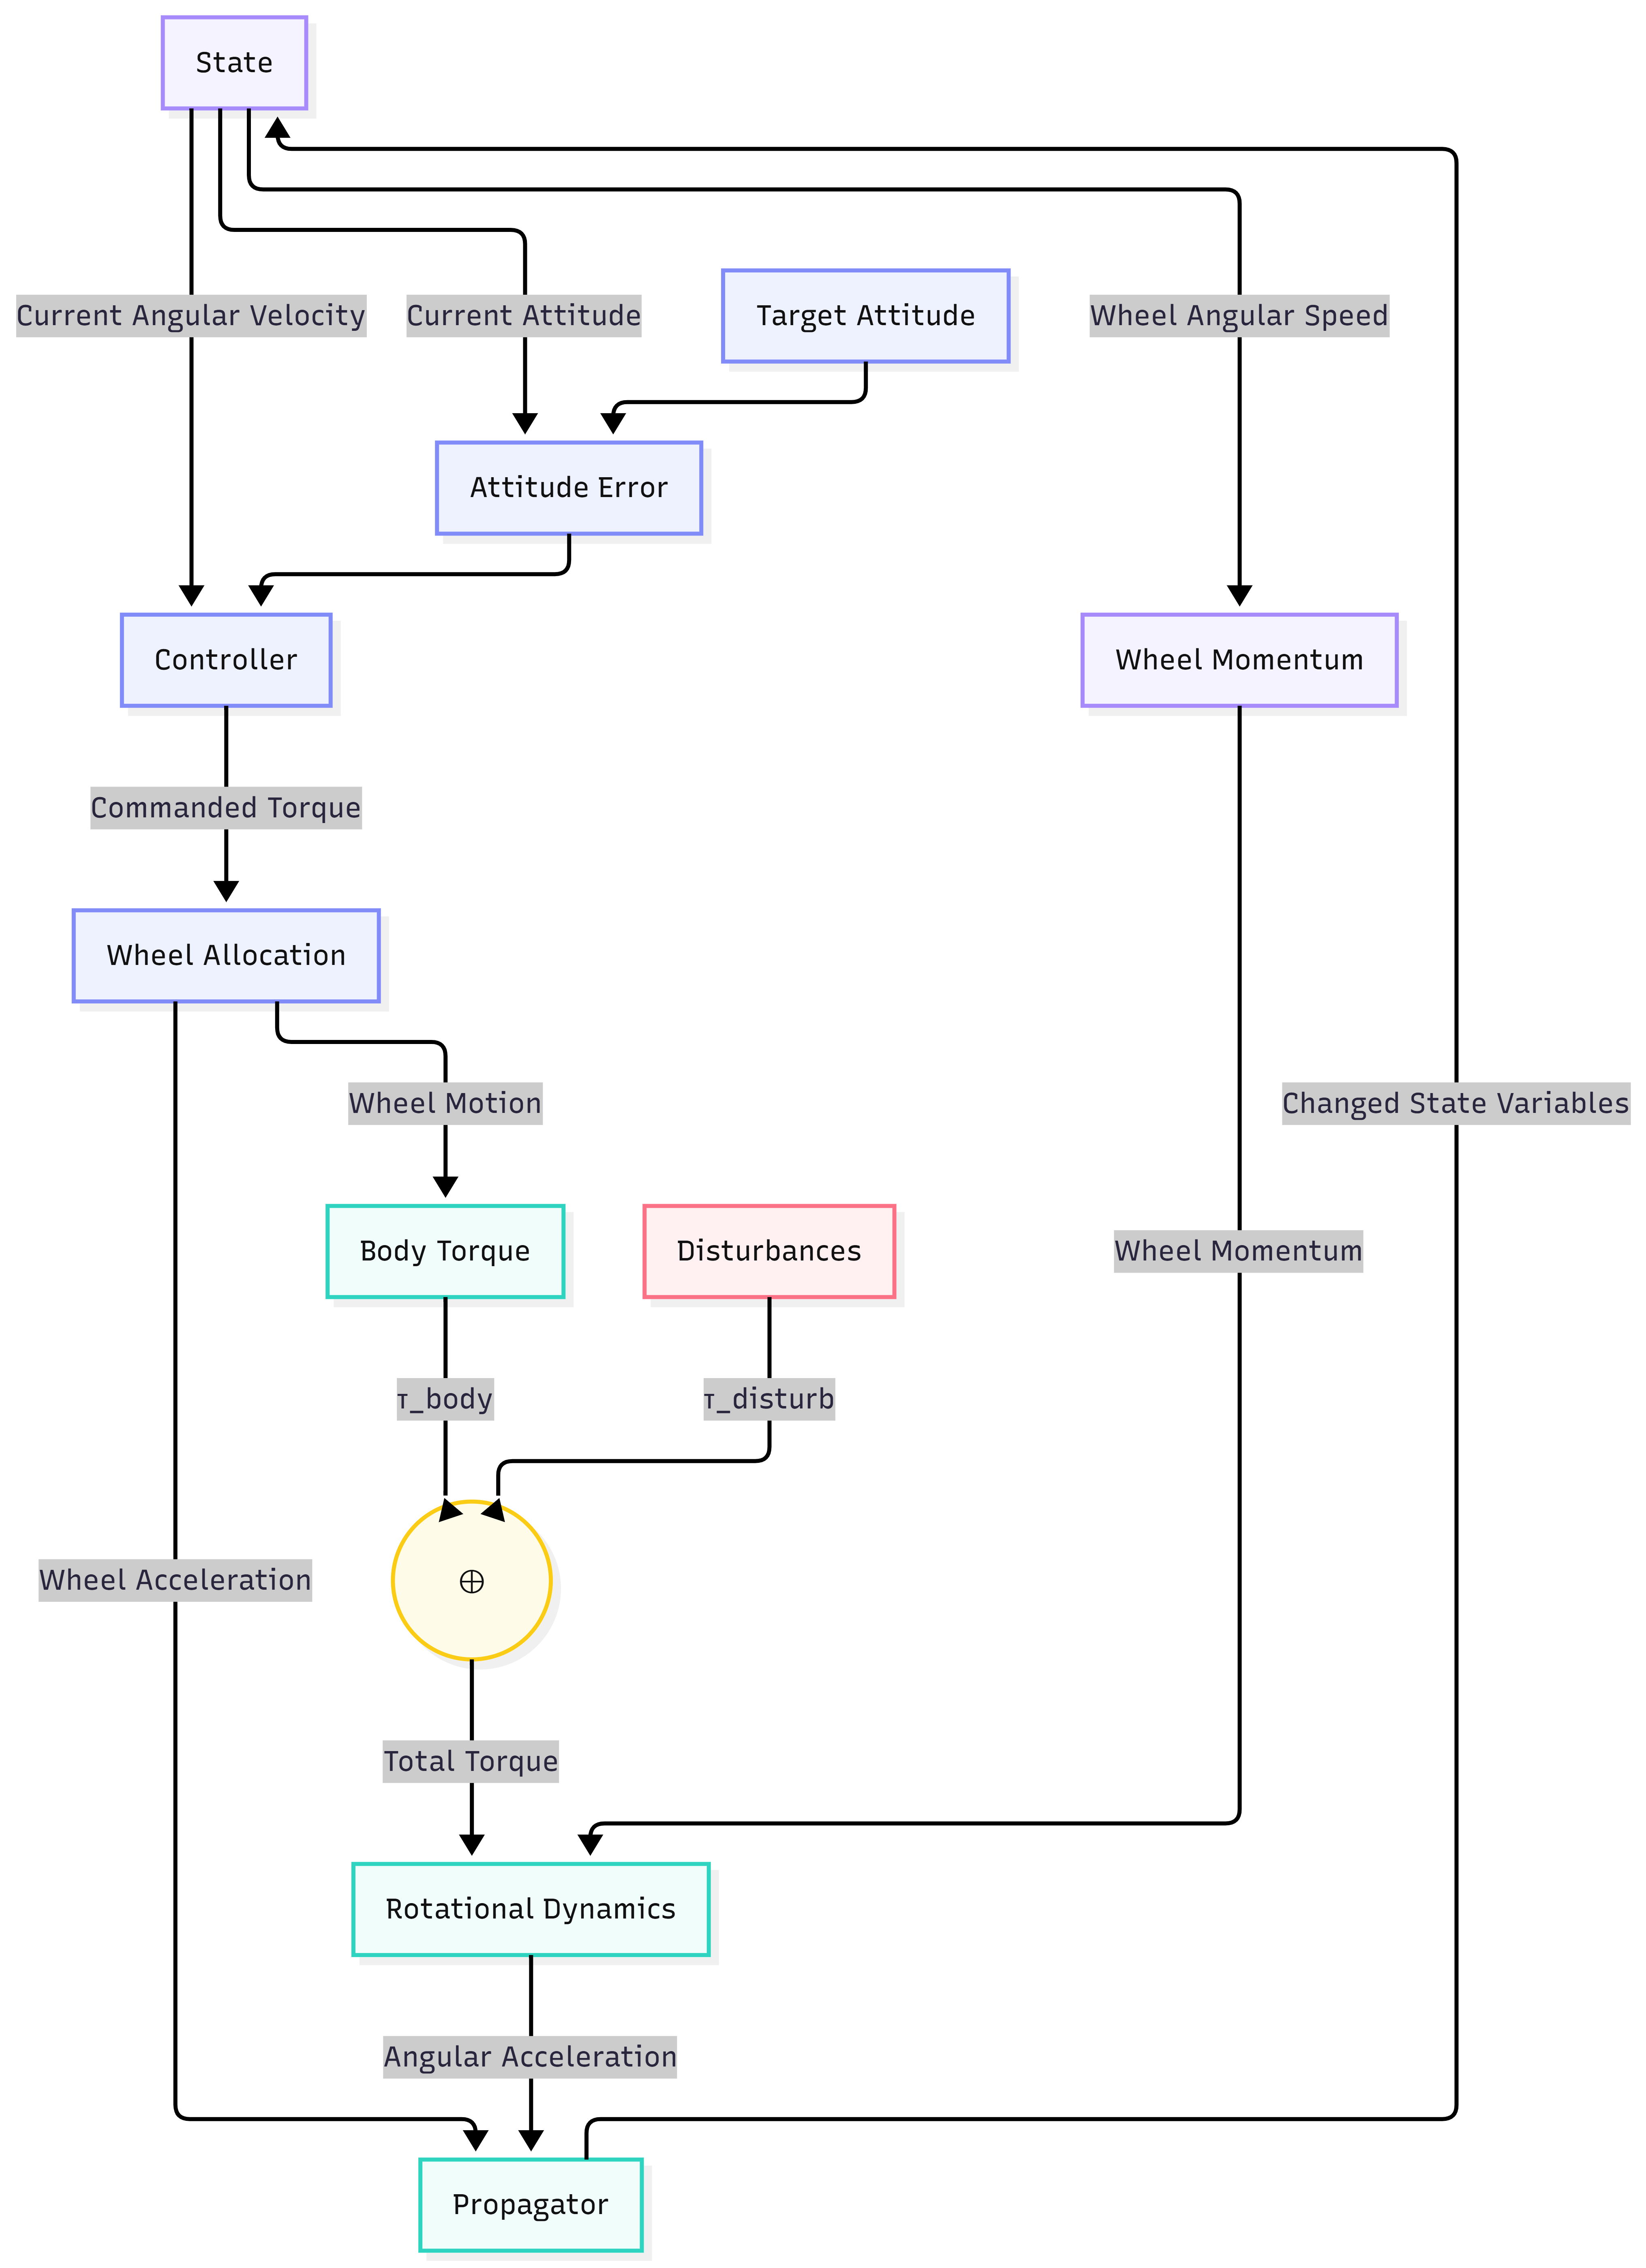
\includegraphics[width=0.95\columnwidth]{figures/control_loop.png}
\caption{Closed-loop signal flow. Attitude error drives the regulator; the
commanded body torque is allocated to the three wheels, and the wheels' stored
momentum $\vect{h}_w$ is fed back into both the rigid-body dynamics and the
decoupling term of \cref{eq:wie}.}
\label{fig:controlloop}
\end{figure}

\subsection{Error quaternion and the sign latch}

Given attitude $\vect{q}$ and target $\vect{q}_t$, the error quaternion is

\begin{equation}
\delta\vect{q} = \vect{q}_t^{-1}\qmul\vect{q}
= \begin{bmatrix}\delta q_0 & \delta\vect{q}_v\T\end{bmatrix}\T,
\label{eq:qerr}
\end{equation}

and the objective is $\delta\vect{q}_v\to\vect{0}$, $\vect{\omega}\to\vect{0}$.
For a unit quaternion the inverse is the conjugate, so this costs three sign
flips and one Hamilton product. The paper works with the regulation case
$\vect{q}_t=[0\ 0\ 0\ 1]\T$, for which the error quaternion is the attitude
quaternion itself; \cref{eq:qerr} is the generalisation to a commanded target,
and is the paper's Eq.~(6).

The complication is that the identity rotation has two representations,
$\delta q_0=\pm1$, because unit quaternions double cover $SO(3)$. Both are
equilibria of the closed loop --- the paper's Remark~4 identifies them as
$(\vect{\omega},\delta\vect{q}_v,\delta q_0)=(\vect{0},\vect{0},\pm1)$ --- and
the sign of the quaternion gain decides which one the system converges to. A
law that ignores this will, started from the far hemisphere, command a rotation
of nearly $360^\circ$ to reach an attitude that is already almost right. This
is unwinding, and it is a property of the parameterisation rather than the
physics.

Remark~5 of the paper fixes it by taking the sign from the initial value of the
scalar part:

\begin{equation}
s \;=\; \sgn\!\left[\delta q_0(t_0)\right],
\qquad \sgn(0)\equiv+1 .
\label{eq:safesign}
\end{equation}

\begin{cautionbox}[The sign is latched once, not evaluated every step]
This is the paper's wording --- ``the sign of the quaternion feedback gain is
defined by the initial value of $q_4$'' --- and the implementation follows it:
\texttt{control/wie.py} freezes $s$ on the first call of a manoeuvre and
\texttt{reset()} clears it. Recomputing $s$ every step is a different
controller. Near $\delta q_0=0$ a recomputed sign chatters, and each flip moves
the system to the other Lyapunov branch of Remark~4, so the function that was
supposed to be decreasing is discarded and replaced mid-manoeuvre. The
stability argument of \cref{sec:wiestab} covers one branch at a time and does
not survive switching between them.
\end{cautionbox}

\subsection{The quaternion feedback regulator}
\label{sec:wie}

The commanded body torque is the paper's Eq.~(9), generalised by Eq.~(14a) and
stated with the sign latch in Remark~5:

\begin{eqbox}
\begin{equation}
\vect{\tau}_\text{cmd}
 = \mu\,\vect{\omega}\times\!\left(\mat{J}\vect{\omega}+\vect{h}_w\right)
 - \mat{K}\,s\,\delta\vect{q}_v
 - \mat{D}\,\vect{\omega}
\label{eq:wie}
\end{equation}
\end{eqbox}

with $\mat{K}$ and $\mat{D}$ constant $3\times3$ positive-definite gain
matrices and $\mu\in\{0,1\}$. The three terms are a nonlinear feedforward
cancellation of gyroscopic coupling, a proportional restoring torque along the
error eigenaxis, and linear rate damping.

\begin{keybox}[This is not a PID with extra terms]
Two of the three terms have no PID analogue. The $\mu$ term is a
\emph{feedforward} cancellation computed from the measured state, not an error
feedback, and its job is to remove a term from the plant rather than to reduce
an error. The latch $s$ is a discrete branch selection, not a gain. And the
paper's law carries no integral term at all: \cref{eq:wie} is the complete
control law, and the stability result of \cref{sec:wiestab} is a statement
about exactly this structure. What makes the law an eigenaxis regulator is the
structural tie $\mat{K}=k\mat{J}$, $\mat{D}=d\mat{J}$ of
\cref{sec:eigenaxis} --- a relationship between the gains and the plant, which
is not a quantity a PID structure has any way to express.
\end{keybox}

Substituting \cref{eq:wie} into the rigid-body dynamics of
\cref{eq:dynamics} gives the closed loop

\begin{equation}
\mat{J}\dot{\vect{\omega}}
 = (1-\mu)\,\vect{\omega}\times\!\left(\mat{J}\vect{\omega}+\vect{h}_w\right)
 - \mat{K}\,s\,\delta\vect{q}_v - \mat{D}\vect{\omega},
\label{eq:wieclosed}
\end{equation}

which is the paper's Eq.~(14a). With $\mu=1$ the gyroscopic term is gone
outright; with $\mu=0$ it is carried, and \cref{sec:wiestab} then constrains
$\mat{K}$ instead.

\subsection{Eigenaxis rotation}
\label{sec:eigenaxis}

Take $\mat{K}=k\mat{J}$ and $\mat{D}=d\mat{J}$ with $k,d>0$ scalars, and
$\mu=1$. Then $\mat{J}$ divides out of \cref{eq:wieclosed} entirely:

\begin{equation}
\dot{\vect{\omega}} = -k\,s\,\delta\vect{q}_v - d\,\vect{\omega}.
\label{eq:wiecl}
\end{equation}

The paper's argument (Sec.~II) is to posit the eigenaxis solution and verify it
closes. Write $\delta\vect{q}_v(t)=\alpha(t)\,\delta\vect{q}_v(0)$ with
$\alpha(0)=1$, i.e.\ assume the error vector keeps its initial direction and
only changes length. From rest, \cref{eq:wiecl} then makes
$\dot{\vect{\omega}}$ parallel to $\delta\vect{q}_v(0)$, so $\vect{\omega}$ is
parallel to it, so the kinematic term
$\skewm{\delta\vect{q}_v}\vect{\omega}$ vanishes identically and the
quaternion kinematics reduce to $\delta\dot{\vect{q}}_v =
\tfrac{1}{2}\delta q_0\vect{\omega}$ --- which is again parallel to
$\delta\vect{q}_v(0)$. The assumed form is consistent, and all three components
of $\delta\vect{q}_v$ obey the same scalar second-order equation. The body
turns about one fixed axis.

\begin{keybox}[What buys the property]
The tie $\mat{K}\propto\mat{J}$, not the values of $k$ and $d$. Any $k,d>0$
gives an eigenaxis rotation; they set how fast, not whether. Conversely,
per-axis gains that break the proportionality --- however carefully tuned ---
destroy it, because then the three components of $\delta\vect{q}_v$ decay at
different rates and the instantaneous rotation axis migrates. This is why the
gain search of \cref{sec:gains} optimises over the two scalars $(k,d)$ rather
than six independent per-axis gains: the larger space does not contain a better
eigenaxis controller, it contains no eigenaxis controller at all.
\end{keybox}

Note the property is the minimum-\emph{angle} path, not the
minimum-\emph{time} path, and it is stated for $\vect{\omega}(0)=\vect{0}$.

\subsection{Stability}
\label{sec:wiestab}

Following Sec.~III of the paper, assume $\mat{K}^{-1}$ exists and
$\mat{K}^{-1}\mat{J}$ is symmetric positive definite, and take

\begin{equation}
V = \tfrac{1}{2}\,\vect{\omega}\T\mat{K}^{-1}\mat{J}\,\vect{\omega}
  + 2\left(1-s\,\delta q_0\right) \;\ge\; 0,
\label{eq:V}
\end{equation}

kinetic energy in a $\mat{K}^{-1}\mat{J}$ metric plus a potential vanishing
only at $s\,\delta q_0=1$. $V$ is positive definite in the error state and
radially unbounded in $\vect{\omega}$. Differentiating along
\cref{eq:wieclosed},

\begin{equation}
\dot{V} = -\,\vect{\omega}\T\mat{K}^{-1}\mat{D}\,\vect{\omega}
 \;+\; (1-\mu)\,\vect{\omega}\T\mat{K}^{-1}
   \skewm{\vect{\omega}}\mat{J}\vect{\omega}.
\label{eq:Vdot}
\end{equation}

The second term is what the paper's analysis is really about, and it vanishes
identically under either of two independent conditions:

\begin{enumerate}[label=\textbf{(\alph*)},leftmargin=*,labelsep=0.5em]
\item $\mu=1$ --- the gyroscopic torque is cancelled exactly, so the term is
absent whatever $\mat{K}$ is; or
\item $\mu=0$ and $\mat{K}$ is chosen so that
\begin{equation}
\mat{K}^{-1} = \alpha\mat{J} + \beta\mat{I},
\qquad \alpha,\beta\ge0,
\label{eq:Kcond}
\end{equation}
which is the paper's Eq.~(17). The $\alpha\mat{J}$ part contracts with
$\skewm{\vect{\omega}}$ to zero because $\skewm{\vect{\omega}}$ is
antisymmetric, and the $\beta\mat{I}$ part vanishes because
$\vect{\omega}\T\skewm{\vect{\omega}}=\vect{0}$.
\end{enumerate}

Under either condition $\dot{V}=-\vect{\omega}\T\mat{K}^{-1}\mat{D}\vect{\omega}$,
which is negative semidefinite whenever $\mat{K}^{-1}\mat{D}>0$. The natural
choice guaranteeing this is $\mat{D}=d\mat{J}$ (the paper's Eq.~(20)).
Asymptotic stability then follows from LaSalle's invariance principle
\cite{khalil}: on $\{\dot{V}=0\}$ we have $\vect{\omega}\equiv\vect{0}$, hence
$\dot{\vect{\omega}}\equiv\vect{0}$, so \cref{eq:wieclosed} forces
$\mat{K}s\,\delta\vect{q}_v=\vect{0}$ and therefore
$\delta\vect{q}_v=\vect{0}$. The largest invariant set is the target attitude,
and the result is global.

\begin{keybox}[Which branch this design uses]
The flown configuration takes branch~(a): $\mu=1$ with
$\mat{K}=k\mat{J}$. That is the only branch that is simultaneously globally
stable \emph{and} eigenaxis, because branch~(b) forbids
$\mat{K}\propto\mat{J}$ --- $\mat{K}^{-1}=(1/k)\mat{J}^{-1}$ is not of the form
$\alpha\mat{J}+\beta\mat{I}$ for any $\alpha,\beta\ge0$ unless $\mat{J}$ is
isotropic. Since $\mat{J}$ is positive definite, every $k,d>0$ satisfies
branch~(a), so the entire two-parameter design space is globally stable by
construction and the gain search of \cref{sec:gains} cannot return an unstable
result. The price, paid in \cref{sec:wierobust}, is that branch~(a) needs
$\mat{J}$ to be known.
\end{keybox}

\paragraph{Remarks 1--3: the constraint on a diagonal plant}
When the body axes are principal axes, $\mat{J}=\diag(J_1,J_2,J_3)$ and
\cref{eq:Kcond} reduces to a per-axis condition on $1/K_i$; only two of the
three quaternion gains may be chosen independently, the third being fixed by
the principal moments (the paper's Eq.~(24)). Because an eigenaxis rotation
wants $\mat{K}$ as close to proportional to $\mat{J}$ as the constraint allows,
Remark~3 selects $\alpha,\beta$ by minimising
$\sum_i\left(\alpha J_i+\beta-1/J_i\right)^2$. The implementation solves this
as an ordinary least-squares fit rather than transcribing the paper's
closed-form Eq.~(26).

\begin{cautionbox}[The least-squares fit returns $\alpha<0$ on this plant]
Fitting \cref{eq:Kcond} to the DEIMoS inertia tensor gives
$\alpha=-2.78\times10^{3}$, $\beta=1.27\times10^{2}$. The negative $\alpha$
violates the nonnegativity the paper attaches to Eq.~(17). The resulting
$\mat{K}^{-1}=\diag(26.2,\,30.6,\,98.3)$ is still positive definite, and since
$\mat{J}$ is diagonal $\mat{K}^{-1}\mat{J}$ is still symmetric positive
definite, so the conclusion of the proof survives --- but it survives by direct
verification, not by the paper's sufficient condition. \texttt{analysis/stability.py}
performs that check and reports which branch a given gain set satisfies. This
only affects the $\mu=0$ cases; the flown $\mu=1$ design is unaffected.
\end{cautionbox}

\paragraph{Remark 6: damping alone sets the achievable decay rate}
With $\mat{K}^{-1}=\alpha\mat{J}+\beta\mat{I}$ and $\mat{D}=d\mat{J}$ the
paper bounds the decay of \cref{eq:V} by
$\dot{V}\ge-2dV$, so

\begin{equation}
V(t) \;\ge\; V(t_0)\,e^{-2d(t-t_0)} .
\label{eq:decay}
\end{equation}

The maximal decay rate is set by $d$ and is \emph{independent of the quaternion
gain}. This is a sharper design statement than it first looks: raising $k$
alone cannot make the closed loop converge faster than \cref{eq:decay} allows,
it can only make the transient stiffer and the peak torque larger. The
saturation behaviour reported in \cref{sec:selectedgains} is the practical
consequence.

\subsection{Gain selection}
\label{sec:wiegains}

Sec.~IV of the paper reduces the gain choice to a second-order form. With
$\mat{K}=k\mat{J}$, $\mat{D}=d\mat{J}$ and $\vect{\lambda}$ the unit eigenaxis,
write $\delta\vect{q}_v=\sin(\phi/2)\,\vect{\lambda}$ and
$\vect{\omega}=\dot{\phi}\,\vect{\lambda}$, where $\phi$ is the eigenangle to
go. \Cref{eq:wiecl} becomes the scalar equation

\begin{equation}
\ddot{\phi} + d\,\dot{\phi} + k\sin(\phi/2) = 0 ,
\label{eq:phi}
\end{equation}

and for $\phi<90^\circ$ the approximation $\sin(\phi/2)\approx\phi/2$ gives the
linear second-order system

\begin{equation}
\ddot{\phi} + d\,\dot{\phi} + \tfrac{k}{2}\,\phi = 0,
\qquad
\omega_n=\sqrt{k/2},
\quad
2\zeta\omega_n = d .
\label{eq:secondorder}
\end{equation}

Inverting, a design point $(\zeta,\omega_n)$ maps to gains by

\begin{eqbox}
\begin{equation}
k = 2\omega_n^2,
\qquad
d = 2\zeta\omega_n .
\label{eq:kdrule}
\end{equation}
\end{eqbox}

\begin{designbox}[The settling-time relation is $8/(\zeta\omega_n)$, not $4/(\zeta\omega_n)$]
The paper is explicit that for $\phi(0)$ approaching $180^\circ$ the standard
small-signal $t_s=4/(\zeta\omega_n)$ underestimates, and a modified relation
\begin{equation}
t_s = \frac{8}{\zeta\omega_n}
\label{eq:ts}
\end{equation}
should be used instead, to account for the nonlinearity of $\sin(\phi/2)$ that
\cref{eq:secondorder} linearised away. Using the small-angle relation on a
large slew is a factor-of-two error in the wrong direction --- it sizes gains
for a manoeuvre that then takes twice as long as intended. DEIMoS's scenarios
run to $152^\circ$, so \cref{eq:ts} is the relation used throughout, in
\texttt{WieRegulator.design()} and in \cref{sec:gains}.
\end{designbox}

\subsection{Robustness to inertia uncertainty}
\label{sec:wierobust}

Sec.~V of the paper addresses what happens when the $\mat{J}$ used by the
controller is not the plant's. Writing $\mat{J}=\mat{J}_n+\Delta\mat{J}$, the
$\mu=1$ cancellation is no longer exact and the closed loop retains

\begin{equation}
\mat{J}\dot{\vect{\omega}}
 = \vect{\omega}\times\Delta\mat{J}\,\vect{\omega}
 - \mat{K}s\,\delta\vect{q}_v - \mat{D}\vect{\omega} .
\label{eq:robust}
\end{equation}

The paper's result is that $\mat{K}=k\mat{I}$ guarantees global stability
whatever $\Delta\mat{J}$ is, because the residual then falls under
branch~(b) of \cref{sec:wiestab} with $\alpha=0$. The price is stated plainly:
``the rotation is not performed about the eigenaxis.''

\begin{keybox}[The central trade of the paper]
Eigenaxis optimality and robustness to inertia error pull in opposite
directions. $\mat{K}=k\mat{J}$ gives the shortest path and needs an accurate
$\mat{J}$; $\mat{K}=k\mat{I}$ tolerates an unknown $\mat{J}$ and gives up the
path. DEIMoS takes the first because its inertia tensor is CAD-extracted and
confirmed diagonal-dominant (\cref{sec:inertia}), which is the condition under
which that choice is defensible.
\end{keybox}

\subsection{The four gain matrices}
\label{sec:fourcases}

Sec.~VI of the paper compares four choices of $\mat{K}$ at a common damping
matrix $\mat{D}=d\mat{J}$, normalising each $\mat{K}$ so that the $y$-axis gain
matches and the cases therefore differ only in the \emph{shape} of $\mat{K}$.
All four are implemented in \texttt{control/wie.py} and reproduced here on the
DEIMoS plant at $\zeta=1$, $t_s=20\unit{s}$, with $\mu=1$ throughout so that
the eigenaxis property is isolated as a pure $\mat{K}$-shape effect (the
paper's Remark~7: with exact decoupling, $\mat{K}$ is unconstrained for
stability).

\begin{cautionbox}[Normalisation is not cosmetic at CubeSat scale]
The paper normalises all four $\mat{K}$ with respect to $K_2$. That step
matters far more here than it does there. Case~1 sets $K_i=k/J_i$, which for
the paper's $\mathcal{O}(10^3)\unit{kg\,m^2}$ inertias produces gains
comparable to the other cases, but for DEIMoS's
$\mathcal{O}(10^{-2})\unit{kg\,m^2}$ inertias produces gains roughly $10^3$
times larger. Run unnormalised, Case~1 saturates the wheels for $99.99\,\%$ of
the manoeuvre and never settles --- a statement about the units, not about the
gain shape. The comparison below is normalised, as the paper's is.
\end{cautionbox}

\begin{table}[!t]
\centering
\caption{The paper's four quaternion gain matrices, normalised to a common
$K_2$ and evaluated on the DEIMoS plant. Deviation is the mean angle between
the instantaneous rotation axis and the initial eigenaxis, on the
$50^\circ$ slew where no wheel saturates.}
\label{tab:fourcases}
\footnotesize
\begin{tabular}{@{}llcc@{}}
\toprule
& $\mat{K}$ & $\mu$ & Deviation \\
\midrule
Case 1 & $k/J_i$ \ (Mortensen \cite{mortensen1968}) & 0 & $22.46^\circ$ \\
Case 2 & $k\mat{I}$ \ (Vadali/Junkins, Wie/Barba)   & 0 & $17.44^\circ$ \\
Case 3 & $(\alpha\mat{J}+\beta\mat{I})^{-1}$        & 0 & $8.16^\circ$ \\
\textbf{Case 4} & $\bm{k\mat{J}}$ \ \textbf{(flown)} & \textbf{1} & $\bm{0.003^\circ}$ \\
\bottomrule
\end{tabular}
\end{table}

\Cref{tab:fourcases} reproduces the paper's ordering exactly: Case~4 is
eigenaxis to three decimal places, Case~3 is the closest of the constrained
forms, and Cases~1 and~2 are visibly non-eigenaxis. It also shows how sharp the
condition is. Case~3's normalised gains,
$\diag(1.29,\,1.10,\,0.343)\times10^{-2}$, differ from Case~4's
$\diag(1.15,\,1.10,\,0.325)\times10^{-2}$ by at most $11\,\%$ per axis, and
that is enough to move the mean deviation from $0.003^\circ$ to $8.16^\circ$.
The eigenaxis property is not something a nearly-proportional $\mat{K}$
nearly achieves.

\begin{cautionbox}[Case numbering]
The numbering above is the paper's. The repository's configuration files use
descriptive names instead --- \texttt{eigenaxis} is the paper's Case~4,
\texttt{near\_eigenaxis} is Case~3, \texttt{robust} is Case~2 and
\texttt{mortensen} is Case~1 --- and a comment in
\texttt{configs/controllers/wie\_eigenaxis.yaml} currently mislabels the
eigenaxis case as ``Case 1''. \TODO{Correct the case number in the two Wie
preset headers so the code and this report agree.}
\end{cautionbox}

\subsection{Departures from the paper on this plant}
\label{sec:departures}

Three of the paper's assumptions do not hold for DEIMoS, and each is handled
explicitly rather than ignored.

\paragraph{The plant is a momentum-exchange system}
The paper assumes an ideal torque actuator, so its plant is
$\mat{J}\dot{\vect{\omega}}=\vect{u}-\vect{\omega}\times\mat{J}\vect{\omega}$
and $\mu=1$ cancels the gyroscopic term outright. DEIMoS stores momentum in the
wheels, and $\vect{h}_w$ sits inside the same cross product
(\cref{eq:dynamics}). Cancelling only the body part leaves
$-\vect{\omega}\times\vect{h}_w$ uncancelled --- a torque that is not along the
error eigenaxis and that \emph{grows} through the manoeuvre, because
$\vect{h}_w$ is exactly what the wheels accumulate in order to perform it.
\Cref{eq:wie} therefore cancels the total momentum $\mat{J}\vect{\omega}+\vect{h}_w$,
which is what the flag \texttt{decouple\_wheel\_momentum} enables.

\begin{keybox}[Measured cost of getting this wrong]
On the $50^\circ$ slew, mean eigenaxis deviation is $3.65^\circ$ with the wheel
term omitted and $0.003^\circ$ with it included --- three orders of magnitude.
Settling time moves by under $1.5\unit{s}$ either way. The defining property of
the control law fails silently while the metric most readers check barely
registers it, which is why \texttt{control/wie.py} raises rather than falling
back to body-only decoupling when $\vect{h}_w$ is not supplied.
\end{keybox}

\paragraph{The actuator saturates}
The paper's analysis assumes the commanded torque is delivered. The wheels cap
at $\tau_\text{max}=4.0\times10^{-3}\unit{N\,m}$ per wheel, and once the
allocation clips, the delivered torque is no longer $\mat{K}s\,\delta\vect{q}_v$
and nothing about the eigenaxis derivation applies. This is the dominant
practical limit on the property and is quantified in \cref{sec:selectedgains};
the clip itself is a per-axis saturation applied before allocation
(\cref{sec:sathandling}).

\paragraph{Integral action is included, gain-scheduled by phase}
\Cref{eq:wie} has no integral term. \texttt{control/wie.py} adds one as an
optional heuristic augmentation,
$\vect{\tau}_\text{cmd}\mathrel{-}=\mat{K}_i\!\int_0^t s\,\delta\vect{q}_v\,dt'$,
kept proportional to $\mat{J}$ ($\mat{K}_i=k_i\mat{J}$) for the same reason
$\mat{K}$ and $\mat{D}$ are: an integral term that is not a scalar multiple of
$\mat{J}$ reintroduces the per-axis asymmetry of \cref{sec:asymmetry} and the
eigenaxis property degrades exactly as it does for a non-proportional
$\mat{K}_p$. It is explicitly outside the Sec.~III
proof --- the integral state adds a dimension \cref{eq:V} does not cover --- so
no global-stability claim is made for it; it is validated numerically instead.

\begin{keybox}[Any nonzero $k_i$ degrades an active slew, so it is switched on only after settling]
Table~\ref{tab:kisweep} sweeps $k_i/k$ on the $152^\circ$ slew. Overshoot grows
from the very first nonzero value tried, and the slew fails to settle within
$120\unit{s}$ once $k_i/k\ge0.003$. The mechanism is ordinary integrator
windup during a fast transient: the accumulator charges while the error is
still large, then discharges against the tail of the manoeuvre, exactly what
the anti-windup clamp of \cref{sec:discrete} limits but cannot eliminate.
DEIMoS therefore runs two configurations, switched by mission phase rather
than by a single always-on gain: \texttt{wie\_eigenaxis.yaml} ($\mat{K}_i=0$)
for an active slew, and \texttt{wie\_eigenaxis\_hold.yaml}
($k_i/k=0.01$, otherwise identical) once the error is already small. This is
ordinary gain scheduling between manoeuvre and fine-pointing phase, not a
limitation of the eigenaxis law, and it is the same trade-off
\texttt{pid\_example.yaml}'s own tuning history records for the PID case
before this report moved to the Wie regulator throughout.
\end{keybox}

\begin{table}[!t]
\centering
\caption{Effect of integral gain ratio $k_i/k$ on \texttt{slew\_160\_40\_30}
($152^\circ$), $120\unit{s}$, otherwise the flown $\mat{K},\mat{D}$.}
\label{tab:kisweep}
\footnotesize
\begin{tabular}{@{}rrr@{}}
\toprule
$k_i/k$ & Final error (deg) & Overshoot (deg) \\
\midrule
$0$      & $0.0018$ & $0.000$ \\
$10^{-5}$ & $0.0093$ & $0.007$ \\
$5\times10^{-5}$ & $0.0456$ & $0.034$ \\
$10^{-4}$ & $0.0907$ & $0.068$ \\
$10^{-3}$ & $0.8267$ & $0.666$ \\
$3\times10^{-3}$ & $2.0122$ & $1.930$ (does not settle) \\
$10^{-2}$ & $3.1310$ & $5.841$ (does not settle) \\
\bottomrule
\end{tabular}
\end{table}

Under the true, much smaller $4.76\times10^{-8}\unit{N\,m}$ per-axis
gravity-gradient bias, the no-integral slew preset's proportional term alone
already leaves a steady-state offset

\begin{equation}
\delta q_{v,i}^{\,ss} = \frac{\tau_{d,i}}{K_{ii}},
\qquad
\delta\theta^{ss} \approx 2\left\|\delta\vect{q}_v^{\,ss}\right\| ,
\label{eq:sserror}
\end{equation}

which measures $0.0018^\circ$ --- two orders of magnitude inside the
$0.1^\circ$ pointing requirement even with no integral action at all.
The hold-phase preset's integral action is therefore not fixing a measured
deficiency on this mission's actual disturbance; it is margin against a larger
one (uncompensated magnetic dipole, aerodynamic torque), and its benefit is
demonstrated directly in \cref{sec:scenarioB} against a bias inflated well
above the gravity-gradient level for exactly that reason.

%==============================================================================
\section{Gain Design}
\label{sec:gains}

The control law of \cref{eq:wie} leaves exactly two numbers free: the scalars
$k$ and $d$ in $\mat{K}=k\mat{J}$, $\mat{D}=d\mat{J}$. Everything else about
the gain matrices is fixed by the plant. This section sizes those two scalars
analytically from the paper's Sec.~IV rule, bounds them by actuator authority,
and then reports what a multi-objective search finds when allowed to move them
freely. The flown design is the analytic one; the search is reported because
what it does to the eigenaxis property is the most informative result in this
chapter.

\subsection{Analytic sizing}
\label{sec:analytic}

\Cref{eq:kdrule,eq:ts} give the design point directly. Choosing $\zeta=1$
(critically damped, so no overshoot is paid for on a large slew) and a target
$t_s=20\unit{s}$ gives $\omega_n = 8/(\zeta t_s) = 0.400\unit{rad/s}$ and hence

\begin{eqbox}
\begin{equation}
\mat{K} = 2\omega_n^2\,\mat{J} = 0.320\,\mat{J},
\qquad
\mat{D} = 2\zeta\omega_n\,\mat{J} = 0.800\,\mat{J} .
\label{eq:gainmap}
\end{equation}
\end{eqbox}

Because $\mat{K}$ and $\mat{D}$ are built from $\mat{J}$ at construction time,
these two scalars are independent of the inertia tensor's numerical values:
when the placeholder tensor was replaced by the CAD-extracted one, the preset
needed no rescaling.

\subsubsection{The unsaturated bandwidth bound}

Peak torque demand occurs at $t=0$, where $\vect{\omega}=\vect{0}$ and the
whole command is the proportional term, $\vect{\tau}_\text{cmd}=-k\mat{J}\,
s\,\delta\vect{q}_v$. Per axis, staying inside the envelope of
\cref{tab:envelope} requires

\begin{equation}
k \;\le\; \frac{u_{\max,j}}{J_{jj}\,|\delta q_{v,j}|} .
\label{eq:bwbound}
\end{equation}

For a worst-case slew with the whole error on one axis at
$\phi_0=90^\circ$, \cref{eq:bwbound} gives $k\le0.222$, i.e.\
$\omega_n\le0.333\unit{rad/s}$ and $t_s\ge24.0\unit{s}$. The $x$ axis binds, as
it does for the momentum envelope, because it is the weakest axis of the
three-wheel cone.

\begin{keybox}[The flown design exceeds the bound, and the bound says exactly where]
At $k=0.320$ the design sits $1.44\times$ above the $90^\circ$ bound.
Rearranging \cref{eq:bwbound} for the largest saturation-free eigenangle at
fixed $k$ gives $\phi_0\le58.7^\circ$. \Cref{tab:satonset} tests that
prediction against the three scenarios: the $50^\circ$ slew sits under the cap
and saturates for exactly zero timesteps, the $79^\circ$ slew sits marginally
over and grazes it at $0.32\,\%$, and the $152^\circ$ slew sits $1.8\times$
over and saturates for $1.28\,\%$. A $t=0$, damping-free, disturbance-free
estimate predicting the onset of saturation to within a fraction of a percent
is a useful check that the gain path and the allocation agree.
\end{keybox}

\begin{table}[!t]
\centering
\caption{Saturation onset predicted by \cref{eq:bwbound} against measurement,
at the flown $k=0.320$. The cap is evaluated on each scenario's actual error
quaternion.}
\label{tab:satonset}
\footnotesize
\begin{tabular}{@{}lrrr@{}}
\toprule
Scenario & $\phi_0$ & $k$ cap & Measured sat. \\
\midrule
\texttt{slew\_40\_30\_25}  & $50.3^\circ$  & $0.581$ & $0.00\,\%$ \\
\texttt{slew\_55\_65\_15}  & $78.6^\circ$  & $0.362$ & $0.32\,\%$ \\
\texttt{slew\_160\_40\_30} & $151.7^\circ$ & $0.179$ & $1.28\,\%$ \\
\bottomrule
\end{tabular}
\end{table}

Accepting brief saturation at the start of the two larger slews is a deliberate
trade: sizing $k$ down to $0.179$ so that even the $152^\circ$ slew never clips
would push $t_s$ past $30\unit{s}$ on every manoeuvre, including the small ones
that never needed it. The consequence for the eigenaxis property is reported in
\cref{sec:selectedgains}, and for requirement R7 in \cref{sec:compliance}.

\subsubsection{Why there is no axis-asymmetry term}
\label{sec:asymmetry}

A controller using one scalar proportional gain $k_p$ on all three axes has a
per-axis bandwidth $\omega_{n,j}=\sqrt{k_p/2J_{jj}}$, which for this inertia
tensor spreads as

\begin{equation}
\frac{\omega_{n,y}}{\omega_{n,x}} = \sqrt{J_{xx}/J_{yy}} = 1.02,
\qquad
\frac{\omega_{n,z}}{\omega_{n,x}} = \sqrt{J_{xx}/J_{zz}} = 1.88 .
\label{eq:asymmetry}
\end{equation}

The roll axis would be $1.88$ times faster than the design axis. An overdamped
axis is sluggish rather than oscillatory, so this is benign for stability, but
it is fatal for the path: the $z$ error is retired first and the instantaneous
rotation axis drifts away from the eigenaxis.

\begin{keybox}[$\mat{K}=k\mat{J}$ is what removes it]
Substituting $K_{jj}=kJ_{jj}$ into $\omega_{n,j}=\sqrt{K_{jj}/2J_{jj}}$ gives
$\omega_n=\sqrt{k/2}$ on every axis, identically. The inertia cancels. This is
the same cancellation as \cref{eq:wiecl} seen in the frequency domain, and it
is why the design has one bandwidth rather than three. Note that the
\emph{torque} bound of \cref{eq:bwbound} remains per-axis --- equal bandwidth
does not mean equal torque demand, and the $x$ axis still binds.
\end{keybox}

\subsection{Multi-objective gain search}
\label{sec:ga}

The analytic route fixes a design point but cannot trade settling time against
control effort against steady-state error, because those three are not
expressible as one $(\omega_n,\zeta)$ pair. An NSGA-II search \cite{deb2002}
(\texttt{tuning/nsga2.py}, \texttt{tuning/objectives.py}) does that directly,
returning a Pareto front rather than a single design.

\begin{itemize}
\item \textbf{Genes.} Two: $k$ and $d$, sampled log-uniformly, with an optional
third for $k_i/k$ when integral action is enabled. Six independent per-axis
gains are deliberately \emph{not} searched: that larger space does not contain
a better eigenaxis controller, it contains no eigenaxis controller at all
(\cref{sec:eigenaxis}).
\item \textbf{Objectives.} ITAE $\int t|\theta_e|\,dt$, steady-state error, and
control effort $\int\|\vect{u}\|\,dt$, all minimised. Torque saturation above a
configurable fraction of timesteps is treated as infeasible and scored
worst-case, so infeasible candidates are dominated out rather than penalised.
\item \textbf{Why ITAE and not settling time.} A settling time capped at the
run duration is the same constant for every candidate that never settles, so
the whole non-settling part of the population ties and selection among them is
random. ITAE is finite and strictly ordered for every candidate, and its $t$
weight makes late error expensive.
\item \textbf{Scoring.} Each candidate is simulated on every scenario in the
set and the objective vectors aggregated worst-case, so the result is not
overfitted to one slew.
\item \textbf{Warm start.} The population is seeded with \cref{eq:gainmap}.
NSGA-II is elitist, so the returned front cannot be dominated by the textbook
design it started from --- the search can only improve on the sizing rule.
\end{itemize}

\begin{designbox}[Searching $(k,d)$ rather than $(\zeta,\omega_n)$]
The two are equivalent by \cref{eq:kdrule}, but constraining the search to move
along the sizing rule would restrict it to a one-dimensional curve and every
rejected candidate would be rejected for disobeying a rule of thumb rather than
for performing badly. Treating $k$ and $d$ as free positive scalars spans the
whole plane and demotes the design rule to a warm start. Because
$\mat{J}\succ0$, every $k,d>0$ satisfies branch~(a) of \cref{sec:wiestab}, so
the entire search space is globally stable by construction and no stability
constraint has to be bolted onto the objectives.
\end{designbox}

\begin{designbox}[Two robustness features the search needed]
A wall-clock deadline stops each seed at a generation boundary, so a fixed
budget produces a finished run rather than a truncated one, and hypervolume
plateau detection stops a seed that has stopped improving.

A per-candidate evaluation timeout was added after one gain vector took
$1800\unit{s}$ to simulate against a $3\unit{s}$ baseline with no exception
raised. Because results are collected in submission order, that one candidate
blocked its entire generation and consumed the whole budget. Candidates
exceeding the timeout are now scored worst-case instead of blocking.
\end{designbox}

\subsection{Selected gains}
\label{sec:selectedgains}

\Cref{tab:gains} lists the flown configuration: the analytic design point of
\cref{eq:gainmap}, unchanged, gain-scheduled by phase between two presets that
share $\mat{K}$ and $\mat{D}$ and differ only in $\mat{K}_i$
(\cref{sec:departures}).

\begin{table}[!t]
\centering
\caption{Flown controller configuration. Both presets share $\mat{K}$,
$\mat{D}$; only $\mat{K}_i$ differs between manoeuvre and hold phase.}
\label{tab:gains}
\footnotesize
\begin{tabular}{@{}lr@{}}
\toprule
\textbf{Parameter} & \textbf{Value} \\
\midrule
Case                      & \texttt{eigenaxis} (paper Case 4) \\
$\mu$                     & $1$ \\
$\mat{K}$                 & $k\mat{J}$, \ $k=0.320$ \\
$\mat{D}$                 & $d\mat{J}$, \ $d=0.800$ \\
$\zeta$, $t_s$ (design)   & $1.0$, \ $20\unit{s}$ \\
$\omega_n$ (all axes)     & $0.400\unit{rad/s}$ \\
Wheel-momentum decoupling & enabled \\
\midrule
\multicolumn{2}{@{}l}{\itshape Manoeuvre phase, \texttt{wie\_eigenaxis.yaml}}\\
$\mat{K}_i$               & $0$ (\cref{tab:kisweep}: any nonzero value overshoots) \\
\midrule
\multicolumn{2}{@{}l}{\itshape Hold phase, \texttt{wie\_eigenaxis\_hold.yaml}}\\
$\mat{K}_i$               & $k_i\mat{J}$, \ $k_i/k=0.01$ \\
Integral limit            & $1.0\times10^{-3}\unit{N\,m}$ \\
\midrule
Integration step $\Delta t$ & $0.01\unit{s}$ \\
\bottomrule
\end{tabular}
\end{table}

\subsubsection{What the search bought, and what it cost}

The NSGA-II front spans a wide range of $(k,d)$, and its endpoints are much
faster than the analytic design. \Cref{tab:tradeoff} re-simulates two
representative front members on the current plant alongside the flown
configuration.

\begin{keybox}[Settling time is bought with the eigenaxis property]
The fastest front member settles the $50^\circ$ slew in $4.12\unit{s}$ against
the flown design's $14.76\unit{s}$, a $3.6\times$ improvement. Over the same
manoeuvre its mean eigenaxis deviation rises from $0.003^\circ$ to
$20.99^\circ$, its peak wheel torque reaches $100\,\%$ of the limit, and its
control effort rises $19\times$. The mechanism is
\cref{eq:bwbound}: $k=7.00$ is $31\times$ the $90^\circ$ cap, so the wheels
clip through the entire opening transient, the delivered torque is no longer
$k\mat{J}\,\delta\vect{q}_v$, and nothing in \cref{sec:eigenaxis} applies any
more. The search was never asked to preserve the eigenaxis property --- it is
not one of the three objectives --- so it spent it.
\end{keybox}

This is also the practical reading of Remark~6 (\cref{eq:decay}): the maximal
decay rate is set by $d$ alone, so raising $k$ far above the torque bound
cannot buy proportionate convergence, it can only raise the peak demand until
the actuator clips. The front's fast endpoint is where that has already
happened.

\begin{table}[!t]
\centering
\caption{Flown analytic design against two NSGA-II front members, all
re-simulated on the current inertia tensor over $120\unit{s}$ with the
gravity-gradient bias enabled. Deviation is the mean angle between the
instantaneous rotation axis and the initial eigenaxis.}
\label{tab:tradeoff}
\footnotesize
\begin{tabular}{@{}lrrr@{}}
\toprule
& Flown & GA fast & GA accurate \\
\midrule
$k$                     & $0.320$ & $7.003$ & $2.237$ \\
$d$                     & $0.800$ & $3.462$ & $0.436$ \\
Implied $\zeta$         & $1.00$  & $0.93$  & $0.21$ \\
\midrule
\multicolumn{4}{@{}l}{\itshape $50^\circ$ slew}\\
Settling time           & $14.76\unit{s}$ & $4.12\unit{s}$  & $17.99\unit{s}$ \\
Saturation              & $0.00\,\%$      & $2.72\,\%$      & $4.02\,\%$ \\
Effort                  & $8.65\!\times\!10^{-3}$ & $1.62\!\times\!10^{-1}$ & $1.07\!\times\!10^{-1}$ \\
Eigenaxis dev.          & $\bm{0.003^\circ}$ & $20.99^\circ$ & $48.45^\circ$ \\
\midrule
\multicolumn{4}{@{}l}{\itshape $152^\circ$ slew}\\
Settling time           & $21.27\unit{s}$ & $11.14\unit{s}$ & $24.63\unit{s}$ \\
Saturation              & $1.28\,\%$      & $7.12\,\%$      & $9.10\,\%$ \\
Eigenaxis dev.          & $\bm{25.95^\circ}$ & $54.75^\circ$ & $53.42^\circ$ \\
\bottomrule
\end{tabular}
\end{table}

\begin{cautionbox}[The flown design loses the property on the largest slew too]
\Cref{tab:tradeoff} is not a claim that the analytic design is eigenaxis
everywhere. On the $152^\circ$ slew it saturates for $1.28\,\%$ of timesteps
and its mean deviation is $25.95^\circ$ --- the property degrades exactly where
\cref{tab:satonset} predicts clipping begins. What the comparison shows is the
ordering: at every operating point the analytic design holds the path better
than the searched gains, and it is the only configuration tested that holds it
\emph{exactly} anywhere. Recovering the property on the largest slew needs
either command shaping to keep the demand inside the envelope
(\cref{sec:limitations}) or a larger torque budget, not a different gain
search.
\end{cautionbox}

%==============================================================================
\section{Actuators}
\label{sec:actuators}

\subsection{Array geometry}

Three identical wheels sit on a cone. Each spin axis is canted
$\theta=\arccos(1/\sqrt{3})=54.7356^\circ$ from body $+z$ and spaced
$120^\circ$ in azimuth, with wheel 1's in-plane projection along body $+y$:

\begin{equation}
\hat{\vect{e}}_i = \begin{bmatrix}
\sin\theta\sin\phi_i & \sin\theta\cos\phi_i & \cos\theta\end{bmatrix}\T,
\label{eq:Amatrix}
\end{equation}

giving the distribution matrix

\begin{equation}
\mat{A} =
\begin{bmatrix}
0 & 0.7071 & -0.7071\\
0.8165 & -0.4082 & -0.4082\\
0.5774 & 0.5774 & 0.5774
\end{bmatrix}.
\label{eq:Amatrix_num}
\end{equation}

Unlike a pyramid's tilt angle, which is a free parameter with a
power-versus-authority optimum \cite{shirazi2014}, $\theta$ here is fixed by
requiring $\mat{A}\T\mat{A}=\mat{I}$, which has a unique solution for a
symmetric three-fold arrangement. There is no tilt-versus-authority trade to
make. The code asserts orthogonality to $10^{-6}$ at construction.

\subsection{Allocation reduces to a transpose}

For a general array, solving $-\mat{A}\vect{\tau}_s=\vect{\tau}_\text{cmd}$ for
the minimum-norm $\vect{\tau}_s$ uses the pseudo-inverse
$\mat{A}\pinv=\mat{A}\T(\mat{A}\mat{A}\T)^{-1}$, and that is what the
allocation code calls for every geometry. For the cone, $\mat{A}$ is square
and $\mat{A}\T\mat{A}=\mat{I}$ forces $\mat{A}\mat{A}\T=\mat{I}$, so

\begin{equation}
\vect{\tau}_s = -\mat{A}\T\vect{\tau}_\text{cmd},
\qquad
\vect{\tau}_w = \mat{A}\mat{A}\T\vect{\tau}_\text{cmd} = \vect{\tau}_\text{cmd}.
\label{eq:allocation}
\end{equation}

Allocation is exact when unsaturated, with no minimum-norm approximation. Using
\texttt{pinv} regardless of geometry means the same code is correct for the
cone, the pyramid and a body-axis array without a branch.

\begin{keybox}[The cost of the missing fourth wheel]
A square invertible $\mat{A}$ has trivial null space. The pyramid's fourth
wheel bought fault tolerance and a free direction in wheel-speed space for
momentum management. The cone loses both, because both came from the same
missing degree of freedom. \Cref{sec:desat} covers momentum management and
\cref{sec:failure} covers the failure case.
\end{keybox}

\subsection{Torque and momentum envelope}
\label{sec:envelope}

With every wheel at its limit, body authority along axis $j$ is
$\sum_i|\mat{A}_{ji}|\,\tau_\text{max}$, and similarly for momentum. The
cone's three-fold layout with wheel 1 along $+y$ is not symmetric under
swapping $x$ and $y$, so all three axes differ.

\begin{table}[!t]
\centering
\caption{Array envelope from \cref{eq:Amatrix_num}, with
$\tau_\text{max}=4.0\times10^{-3}\unit{N\,m}$ and
$h_\text{max}=7.288\times10^{-3}\unit{N\,m\,s}$.}
\label{tab:envelope}
\footnotesize
\begin{tabular}{@{}llr@{}}
\toprule
\textbf{Quantity} & \textbf{Expression} & \textbf{Value} \\
\midrule
Torque, $x$   & $\sqrt{2}\,\tau_\text{max}$    & $5.657\times10^{-3}\unit{N\,m}$ \\
Torque, $y$   & $2\sin\theta\,\tau_\text{max}$ & $6.532\times10^{-3}\unit{N\,m}$ \\
Torque, $z$   & $3\cos\theta\,\tau_\text{max}$ & $6.928\times10^{-3}\unit{N\,m}$ \\
Momentum, $x$ & $\sqrt{2}\,h_\text{max}$       & $1.031\times10^{-2}\unit{N\,m\,s}$ \\
Momentum, $y$ & $2\sin\theta\,h_\text{max}$    & $1.190\times10^{-2}\unit{N\,m\,s}$ \\
Momentum, $z$ & $3\cos\theta\,h_\text{max}$    & $1.262\times10^{-2}\unit{N\,m\,s}$ \\
\bottomrule
\end{tabular}
\end{table}

The $x$ axis is the tightest. With $\theta$ fixed by orthogonality there was no
opportunity to equalise the axes the way a pyramid's tilt angle allows, and
\cref{sec:analytic} sizes against this weakest axis.

\subsection{Saturation handling}
\label{sec:sathandling}

Each wheel clips its motor command to $|\tau_{s,i}|\le\tau_\text{max}$. The
speed limit uses a sign-aware rule rather than a plain clamp: a wheel at or
past $\Omega_\text{max}$ has any further \emph{accelerating} torque zeroed,
modelling the motor's back-EMF cutoff, while decelerating torque stays fully
available. A pinned wheel can therefore recover, which a symmetric clamp would
not allow.

\begin{designbox}[Saturate after allocation, not before]
Clipping $\vect{\tau}_\text{cmd}$ before allocation would assume all three
wheels saturate together, which is not generally true, and would hide the case
where one wheel is pinned while the others have margin. Saturating per wheel
and recomputing the delivered body torque also changes the \emph{direction} of
the applied torque, not only its magnitude, and that change is physically real.
\end{designbox}

\subsection{Magnetorquer desaturation}
\label{sec:desat}

Since $\mathrm{null}(\mat{A})=\{\vect{0}\}$, no redistribution of wheel speeds
produces zero body torque, and momentum the wheels accumulate can only be
removed by an actuator that is not one of them. Three orthogonal magnetorquers
do that; the simulation models them with a single, axis-uniform
$m_\text{max}=0.2\unit{A\,m^2}$ at $0.2\unit{W}$, a placeholder pending the
real hardware design in \cref{sec:cad_mtq}, which gives distinct rod and coil
limits and the orbit-averaged desaturation time constant.

A rod carrying dipole $\vect{m}$ in field $\vect{B}$ produces
$\vect{\tau}_\text{mtq}=\vect{m}\times\vect{B}$. The implemented law
(\texttt{actuators/magnetorquers.py}) is the standard cross-product dump:

\begin{eqbox}
\begin{equation}
\vect{m} = \mathrm{clip}\!\left(\frac{k_\text{desat}}{\|\vect{B}\|^2}\,
\vect{h}_w\times\vect{B},\ \pm m_\text{max}\right)
\label{eq:mtqlaw}
\end{equation}
\end{eqbox}

Substituting into $\vect{\tau}=\vect{m}\times\vect{B}$ and expanding the triple
product gives $\vect{\tau} = -k_\text{desat}\,\vect{h}_{w\perp}$, the component
of stored momentum perpendicular to the field. The attitude controller holds
pointing against that torque by giving up wheel momentum, which is the
mechanism that empties the wheels. Only the perpendicular component is
reachable at any instant, so dumping relies on $\vect{B}$ rotating through the
body frame over an orbit.

Engagement uses a hysteresis latch: the rods switch on when $\|\vect{h}_w\|$
exceeds a threshold set as a fraction of single-wheel momentum capacity, and
off at a lower fraction of that threshold, so the system does not chatter at
the boundary. The geomagnetic field comes from a tilted-dipole model in
\texttt{dynamics/environment.py}, evaluated along the circular reference orbit
and rotated into the body frame.

Available torque is $m_\text{max}B_0 = 6.24\times10^{-6}\unit{N\,m}$, three
orders below wheel authority and comparable to the gravity-gradient
disturbance. That is the intended sizing, and it matches standard CubeSat
practice \cite{sidi,wertz}: a desaturation actuator wins a slow race against a
slow disturbance, averaged over orbits, rather than competing with the wheels
on response time. \Cref{sec:desat_result} reports the measured
result.

\subsection{Discrete-time implementation}
\label{sec:discrete}

At each control instant the loop forms $\delta\vect{q}$ and applies the sign
correction, evaluates the control law, allocates by \cref{eq:allocation},
saturates per wheel, recomputes the delivered body torque, and holds that
constant across all four RK4 sub-stages. The desaturation loop runs separately,
since it works against a slowly rotating field rather than the attitude error.
\Cref{fig:blockdiagram} shows the path.

%------------------------------------------------------------ WIDE FIGURE ----
\begin{figure*}[!t]
\centering
\begin{adjustbox}{max width=\textwidth}
\begin{tikzpicture}[
  node distance=13mm and 13mm,
  blk/.style={draw=black,rounded corners=2pt,
              align=center,font=\footnotesize,inner sep=4pt,
              minimum height=12mm,text width=29mm},
  plant/.style={blk,very thick,text width=33mm},
  sig/.style={-{Latex[length=2mm]},draw=black,thick},
  fb/.style={-{Latex[length=2mm]},draw=black,thick,dashed}]

\node[blk] (ref) {Target attitude\\$\vect{q}_t$};
\node[blk,right=of ref] (err) {Error quaternion\\\cref{eq:qerr}, \cref{eq:safesign}};
\node[blk,right=of err] (ctrl) {Control law\\\cref{eq:wie}};
\node[blk,right=of ctrl] (alloc) {Allocation\\\cref{eq:allocation}};

\node[blk,below=of alloc] (sat) {Per-wheel\\saturation};
\node[plant,left=of sat] (plant) {Plant\\\cref{eq:kinematics}, \cref{eq:dynamics}\\RK4 with ZOH};
\node[blk,left=of plant,dashed] (mtq)
   {Magnetorquer\\desaturation\\\cref{eq:mtqlaw}};

\draw[sig] (ref) -- (err);
\draw[sig] (err) -- node[above,font=\scriptsize]{$\delta\vect{q}$} (ctrl);
\draw[sig] (ctrl) -- node[above,font=\scriptsize]{$\vect{\tau}_\text{cmd}$} (alloc);
\draw[sig] (alloc) -- node[right,font=\scriptsize]{$\vect{\tau}_s$} (sat);
\draw[sig] (sat) -- node[above,font=\scriptsize]{$\vect{\tau}_w$} (plant);
\draw[sig] (mtq) -- node[above,font=\scriptsize]{$\vect{\tau}_\text{mtq}$} (plant);
\draw[fb] (plant.north) -- ++(0,6mm)
  -| node[right,font=\scriptsize,align=left,pos=0.25]
     {$\vect{q},\vect{\omega},\vect{\Omega}$ held for $T_c$} (err.south);
\draw[fb] (plant.south) -- ++(0,-6mm) -| node[below,font=\scriptsize,pos=0.25]{$\vect{h}_w$} (mtq.south);
\end{tikzpicture}
\end{adjustbox}
\caption{Closed-loop signal path for one control instant. Solid arrows are the
forward path; dashed arrows are state feedback. The wheel command is held
constant across the four RK4 sub-stages. The desaturation loop is driven by
stored wheel momentum rather than attitude error and runs on its own schedule.}
\label{fig:blockdiagram}
\end{figure*}

%==============================================================================
\reportpart{III}{Mechanical Design}

\section{Mechanical Design and CAD}
\label{sec:cad}

\NOTE{Authored by Tulika Chowdhury.}

This section documents the mechanical design and supplies the mass properties
the simulation depends on. It supersedes the four-wheel pyramid CAD carried in
earlier drafts: the structural architecture, wheel array, magnetorquer
hardware, solar array and mass properties below are all built around the
three-wheel orthogonal cone that \cref{sec:actuators} specifies, so the
long-standing CAD/code mismatch flagged in earlier revisions of this report is
resolved for everything except two items noted where they arise --- the exact
new total mass, and a small numerical gap between this section's inertia
tensor and the one the control design in \cref{sec:mission} was already built
on (\cref{sec:inertia} quantifies it rather than silently absorbing it).

\subsection{Structural architecture}
\label{sec:cad_structure}

The primary structure follows commercial 3U practice (ISISpace, Pumpkin): four
hard-anodised aluminium corner rails run the full $340.5\unit{mm}$ length and
form the only mechanical interface to the deployer, per the Cal Poly CubeSat
Design Specification \cite{cds}. The rails carry the launch loads; the internal
stack of end caps and bulkheads is clamped separately by four full-length
threaded rods at $(\pm37,\pm37)\unit{mm}$, following the PC/104 reference
architecture. Decoupling the stack from the rails this way keeps the rail ends
free for the deployment switches, which the specification requires at the
$\pm Z$ ends.

Four Al 6061 shear panels close the side faces, recessed $0.5\unit{mm}$ inside
the rail plane so the rails stay the outermost surface. This replaces the
truss panels of the mid-evaluation design: shear panels give more resistance to
torsional strain, and the panels are detachable, which the truss design did
not offer as cleanly. High-mass components (wheels, battery) mount to the
bulkheads and rails rather than the panels, avoiding threaded-insert pull-out,
the usual failure mode for panel-mounted equipment.

Two bulkheads divide the interior into bays: a central bulkhead ($3\unit{mm}$,
$z=0$) carries the wheel array at the spacecraft's centre of mass, and an upper
bulkhead ($2.5\unit{mm}$) carries the avionics and battery. The payload
telescope occupies the lower bay and exits through the nadir end cap. The
payload (nadir) and the avionics/battery stack (zenith) sit at opposite ends
so they counterbalance about the centre, with the wheels on-axis at the
centre.

\begin{figure}[!t]
\centering
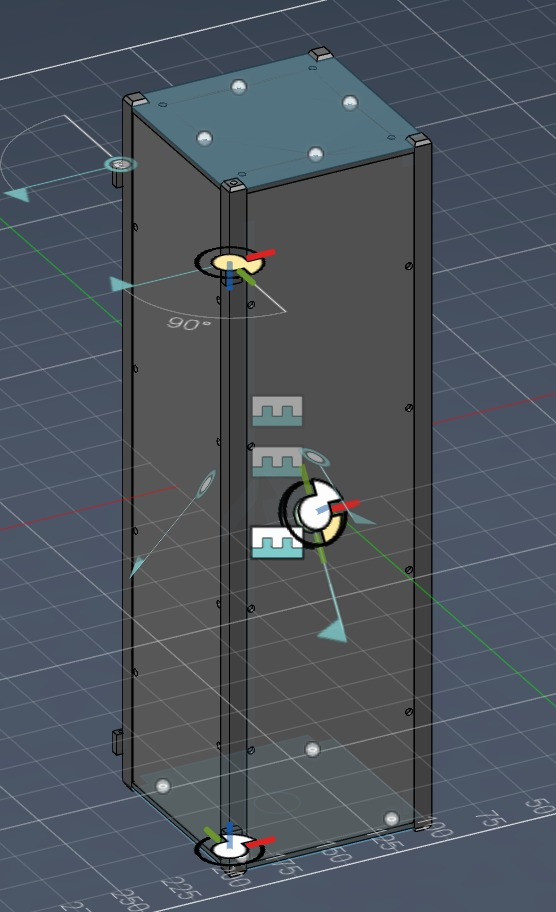
\includegraphics[width=\columnwidth]{figures/cad_chassis.jpg}
\caption{3U CubeSat chassis with shear side panels and rail structure.}
\label{fig:cad_chassis}
\end{figure}

\subsection{Reaction wheel assembly and mounting}
\label{sec:cad_rwa}

The array is three wheels in a mutually orthogonal set, each tilted
$\theta=\arccos(1/\sqrt3)\approx54.74^\circ$ from $+z$ and spaced $120^\circ$
apart in azimuth ($0^\circ,120^\circ,240^\circ$) --- the CAD counterpart of
\cref{eq:Amatrix,eq:Amatrix_num} and, unlike the earlier pyramid, an exact
match to what the simulation flies.

\begin{figure}[!t]
\centering
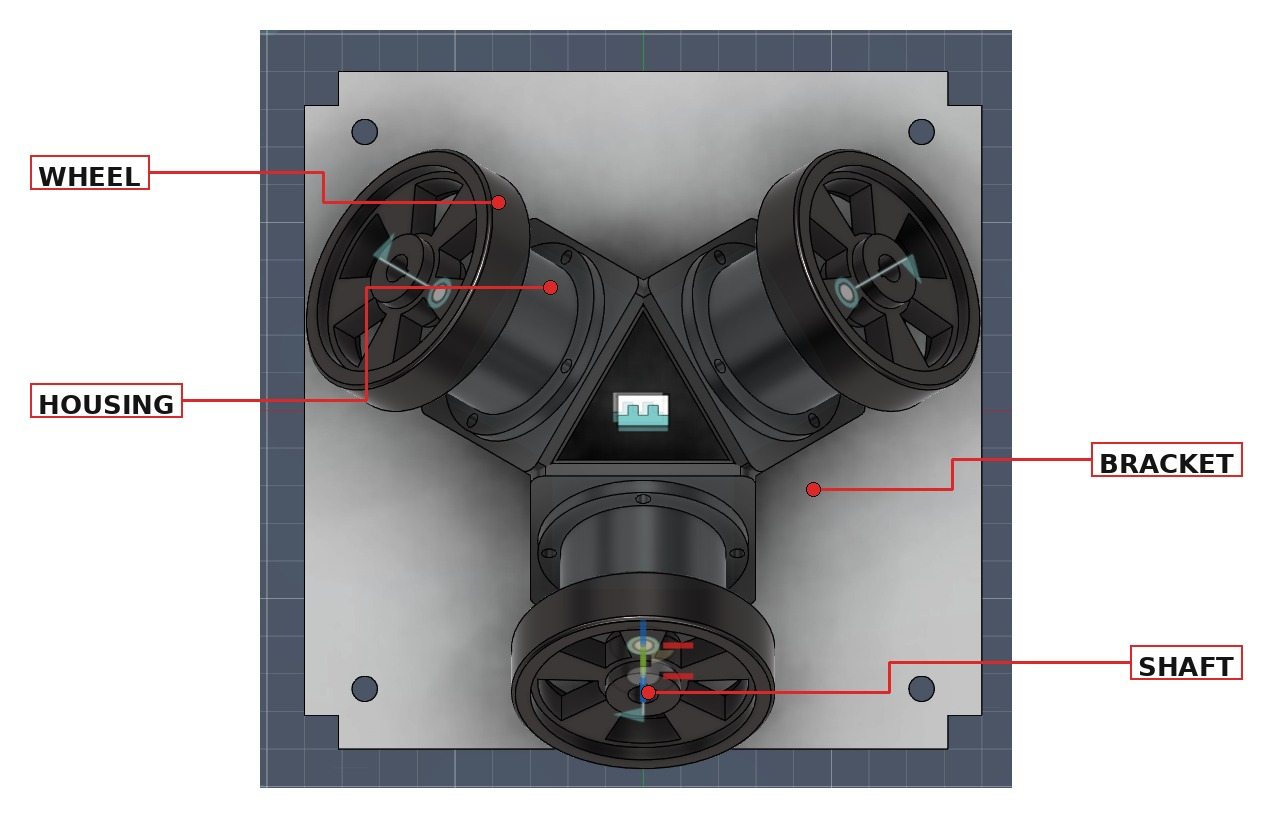
\includegraphics[width=\columnwidth]{figures/cad_rwa.jpg}
\caption{Reaction-wheel assembly, orthogonal configuration. Three wheels at
$120^\circ$ azimuth, each canted $54.74^\circ$ from $+z$, on a common bracket.}
\label{fig:cad_rwa}
\end{figure}

\begin{figure}[!t]
\centering
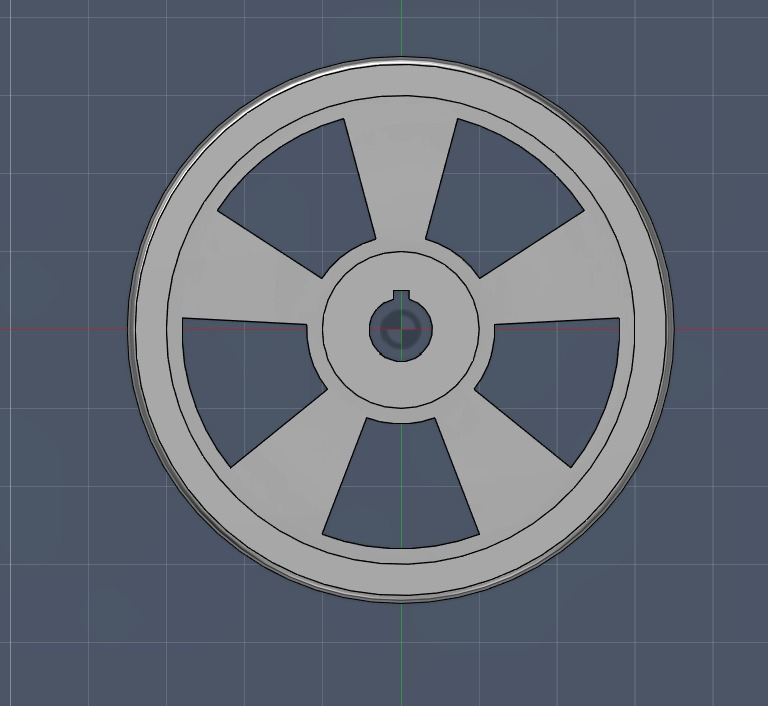
\includegraphics[width=0.72\columnwidth]{figures/cad_wheel.jpg}
\caption{Reaction-wheel rotor. The spoked web places mass at the rim, which is
what makes $I_w$ large for a given wheel mass and sets the momentum envelope of
\cref{tab:envelope}.}
\label{fig:cad_wheel}
\end{figure}

Each wheel is driven by a Maxon ECX Flat 22L brushless motor \cite{maxon},
chosen for its flat form factor (fits the assembly inside the 3U envelope
without extending the wheel bay), brushless construction (no brush wear over a
mission where the wheels run near-continuously in hold mode), fine repeatable
torque control with integrated Hall-sensor speed feedback, and low mass at
$22\unit{mm}$ diameter.

The flywheel uses a 5-spoke design rather than a solid disc: for equal total
mass, concentrating material at the rim gives more spin-axis inertia than a
solid disc, so more stored momentum per gram of flywheel. Each flywheel gives
$I_w=5.8\times10^{-6}\unit{kg\,m^2}$ at $31.116\unit{g}$, the value
\cref{tab:massprops} already carries. Each wheel mounts on an inclined bracket
whose face-normal tilt ($35.26^\circ$, the complement of $54.74^\circ$) sets
the cant; the bracket transfers reaction torque into the central bulkhead
through a bolted base flange and four motor-mount screws.

\begin{figure}[!t]
\centering
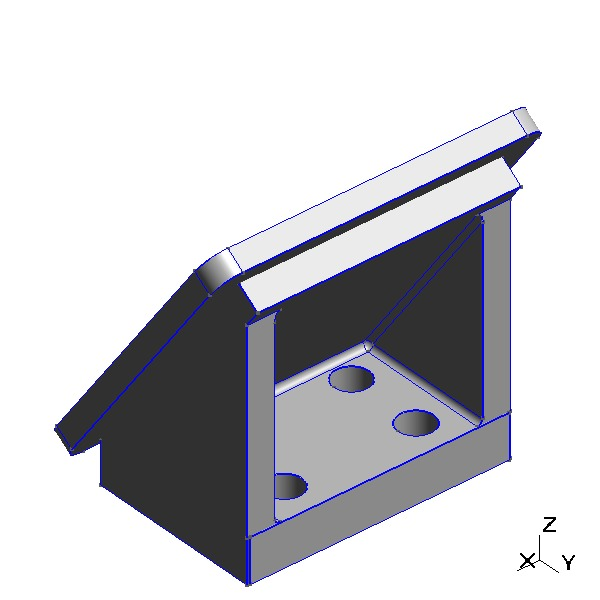
\includegraphics[width=\columnwidth]{figures/cad_bracket.jpg}
\caption{Single reaction wheel and mounting bracket.}
\label{fig:cad_bracket}
\end{figure}

\subsection{Magnetorquer hardware}
\label{sec:cad_mtq}

\Cref{sec:desat} gives the desaturation law; this subsection sizes the rods it
drives. The layout is two torque rods along body $X$/$Y$ plus one flat air-core
coil on the top bulkhead for $Z$, since a rod of useful length does not fit
along the short axis.

The X/Y rods use a ferromagnetic (steel) core with a copper winding: a
high-permeability core concentrates flux and amplifies the achievable dipole
per turn and per amp, so a core is worth the mass a plain air coil would save.
Because the rod is finite, not infinite, its effective permeability is set by
the geometry through the demagnetising factor: at aspect ratio 15
($60\times4\unit{mm}$), $N_d=0.0107$ and the effective rod permeability is
$\mu_\text{rod}\approx86$ from a relative core permeability of $\mu_r=1000$.
Copper is used for both windings for its low resistivity, which minimises
resistive loss for a given dipole. The $Z$ coil is air-core: a ferromagnetic
core has no benefit in a large flat loop and would only add mass, so that axis
relies on turns and enclosed area alone.

Sizing followed the environmental disturbance budget of \cref{tab:disturbances}
at $500\unit{km}$: gravity gradient, aerodynamic drag, solar pressure and the
spacecraft's own residual magnetic dipole (dominant, assuming a residual of
$0.01\unit{A\,m^2}$) total $\approx469\unit{nN\,m}$. Countering that with a
$2\times$ margin at the minimum field $B=25\unit{\mu T}$ requires
$\approx0.038\unit{A\,m^2}$ per axis; \cref{tab:magnetorquer} gives the design
actually built to that requirement, with margin over it on both geometries.

\begin{table*}[!t]
\centering
\caption{Magnetorquer design points. Combined worst-case power draw across all
three axes is under $120\unit{mW}$.}
\label{tab:magnetorquer}
\footnotesize
\begin{tabularx}{\textwidth}{@{}lXlccccc@{}}
\toprule
\textbf{Axis} & \textbf{Geometry} & \textbf{Winding} & \textbf{Current} &
\textbf{Resistance} & \textbf{Power} & \textbf{Dipole} & \textbf{Margin} \\
\midrule
X/Y rod & $60\times4\unit{mm}$ steel core, $14\unit{mm}$ OD copper coil,
  $50\unit{mm}$ winding & 600 turns AWG28 & $100\unit{mA}$ & $\approx2.3\,\Omega$
  & $\approx23\unit{mW}$ & $0.065\unit{A\,m^2}$ & $+70\,\%$ \\
Z coil & $64\times64\unit{mm}$ rounded-square air coil, $6\times6\unit{mm}$
  bundle & 150 turns AWG28 & $100\unit{mA}$ & $\approx7.3\,\Omega$ &
  $\approx73\unit{mW}$ & $0.0504\unit{A\,m^2}$ & $+32.6\,\%$ \\
\bottomrule
\end{tabularx}
\end{table*}

\begin{cautionbox}[The simulation currently models one dipole limit, not two]
\Cref{tab:massprops,sec:desat} carry a single, axis-uniform
$m_\text{max}=0.2\unit{A\,m^2}$, an assumption pending exactly this hardware
design. The design above gives $0.065\unit{A\,m^2}$ on X/Y and
$0.0504\unit{A\,m^2}$ on Z, both well below the placeholder and not equal to
each other. \texttt{MagnetorquerArray} currently clips to one scalar limit for
all three axes; the more accurate value to use there today is the smaller of
the two, $0.0504\unit{A\,m^2}$, since a uniform model should use the binding
axis rather than the more generous one. \TODO{Extend
\texttt{actuators/magnetorquers.py} to accept a per-axis limit (a length-3
array clips elementwise with no other change to the law) and re-run
\cref{sec:desat_result} against it; the desaturation results in this report
were produced under the $0.2\unit{A\,m^2}$ placeholder and have not yet been
re-verified against either real figure.}
\end{cautionbox}

The decay-time-constant result already stated in \cref{sec:desat},
$\vect{\tau}=-k_\text{desat}\vect{h}_{w\perp}$, describes the instantaneous
perpendicular component. Orbit-averaging as $\vect{B}$ sweeps through the body
frame ($\langle\sin^2\theta\rangle=2/3$) gives the decay of the full stored
momentum vector,
\begin{equation}
\|\vect{h}_w(t)\| \approx \|\vect{h}_w(0)\|\,e^{-t/\tau_c},
\qquad
\tau_c = \frac{3}{2k_\text{desat}},
\label{eq:mtqtau}
\end{equation}
which for the $k_\text{desat}=5\times10^{-3}\unit{s^{-1}}$ used in this project
gives $\tau_c\approx300\unit{s}$, about $5\,\%$ of one orbital period. Per orbit
the disturbance budget above delivers $\approx2.66\times10^{-3}\unit{N\,m\,s}$
of momentum to absorb; a target time constant of one fifth of an orbit
($\approx1135\unit{s}$) would set $k_\text{desat}\approx1.32\times10^{-3}
\unit{s^{-1}}$, slower than the value actually used and left as a tuning note
rather than a change, since \cref{sec:desat_result} already demonstrates
desaturation working at the faster rate.

\subsection{Materials and mass budget}
\label{sec:cad_mass}

Aluminium alloys dominate the load-bearing structure: 6061 where machinability
matters, 7075 where stress concentration is higher. The flywheel rim is
stainless steel, to maximise rim density and spin-axis inertia for a given
flywheel mass. The avionics and payload stack is modelled as FR4 PCB with
assorted components.

\begin{cautionbox}[Mass has grown with the redesign; the new total is not yet tabulated]
The three-wheel cone and the deployable solar array of \cref{sec:cad_solar}
both add mass the earlier four-wheel component budget did not carry, so that
budget (and its $1.765\unit{kg}$ total) no longer applies and is not
reproduced here. \Cref{tab:massprops}'s $m=3.9\unit{kg}$ therefore remains an
assumption, not a CAD measurement, until the mass budget is regenerated
component-by-component against the current design and \texttt{SPACECRAFT\_
MASS\_KG} is set from that export rather than the reverse.
\end{cautionbox}

\subsection{Deployable solar array and power budget}
\label{sec:cad_solar}

Power comes from a hybrid array: two deployable wings plus body-mounted cells.
Each wing is an FR4 substrate carrying triple-junction GaAs cells, stowed flat
against a side face within the CDS deployable allowance and released by a
burn-wire hold-down onto a hinge (\cref{fig:cad_solar}). The wings are
constrained by the CubeSat's own hold-down, not the dispenser walls, as the
specification requires.

\begin{figure}[!t]
\centering
\begin{subfigure}[t]{0.47\columnwidth}
\centering
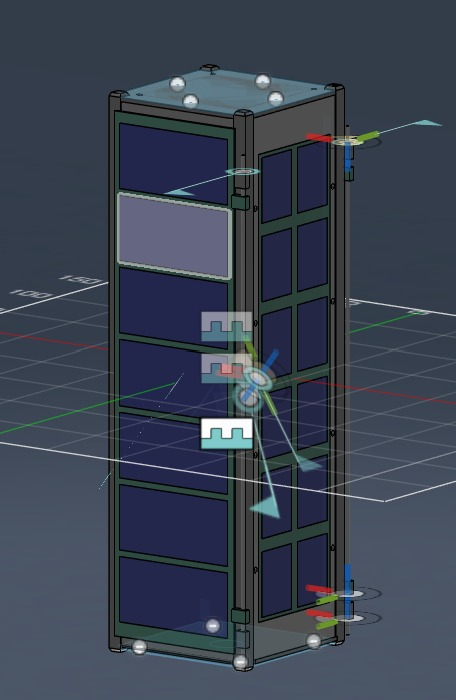
\includegraphics[width=\textwidth]{figures/cad_solar_stowed.jpg}
\caption{Stowed}
\end{subfigure}
\hfill
\begin{subfigure}[t]{0.47\columnwidth}
\centering
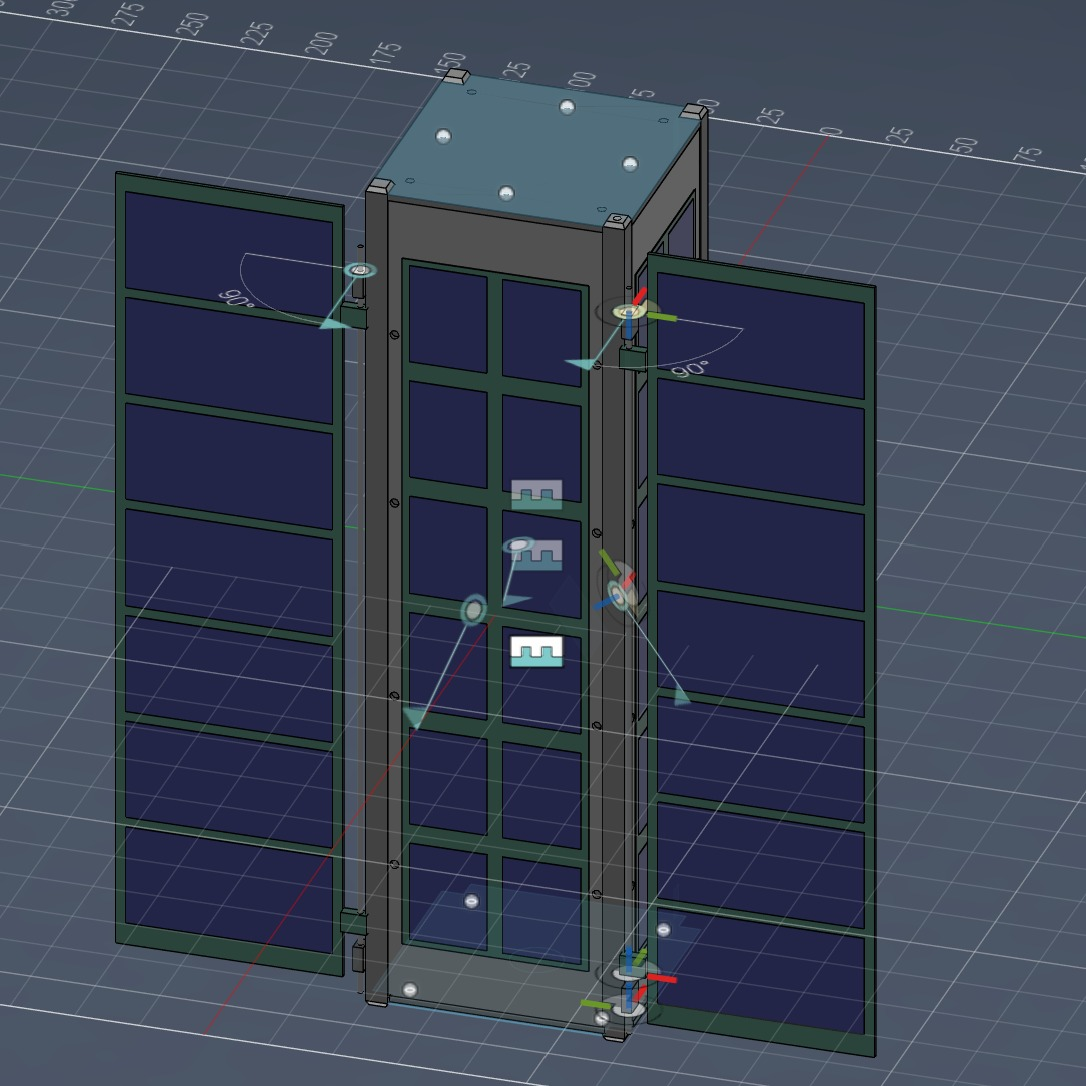
\includegraphics[width=\textwidth]{figures/cad_solar_deployed.jpg}
\caption{Deployed}
\end{subfigure}
\caption{Deployable solar wing, stowed vs.\ deployed.}
\label{fig:cad_solar}
\end{figure}

The array carries 62 triple-junction GaAs cells (28\,\% BOL efficiency)
totalling $1024\unit{cm^2}$: $448\unit{cm^2}$ across the two wings (14 cells,
$80\times40\unit{mm}$) and $576\unit{cm^2}$ body-mounted across the four side
faces (48 cells, $30\times40\unit{mm}$). The nadir face carries no cells
(payload aperture) and the zenith cap is bare (structural interfaces).
Body-mounted cells alone would average only $\approx2\unit{W}$ per orbit --- a
negative budget, and the commonest CubeSat power failure --- so the wings are
mission-critical: they roughly triple the sun-facing area.

At normal incidence the theoretical peak is $\approx39\unit{W}$
($1361\unit{W/m^2}\times1024\unit{cm^2}\times0.28$, matching
\texttt{constants.py}'s \texttt{SOLAR\_PEAK\_POWER\_W} exactly). After eclipse
($\approx38\,\%$ of each orbit) and incidence-angle losses, orbit-averaged
generation is $\approx8.5\unit{W}$, again matching the constant the simulation
uses. The estimated orbit-average load is dominated by the ADCS: operating the
wheels in a momentum-hold-dominant profile with slew transients buffered by the
battery draws $\approx2.5$--$3\unit{W}$; other subsystems and EPS losses bring
the total to $\approx4.7$--$5.2\unit{W}$, close to the itemised $4.3$--$5.6
\unit{W}$ (with margin) in \cref{tab:disturbances}'s companion power analysis.
Generation against load gives a margin of roughly $1.6$--$1.8\times$, inside
standard CubeSat practice ($1.3$--$2\times$) and with headroom for cell
degradation.

\subsection{Inertia tensor and centre of mass}
\label{sec:inertia}

The tensor was exported from Fusion 360 in $\mathrm{g\,mm^2}$ and converted.
Deploying the wings moves mass outboard, so the CAD reports both
configurations; the controller operates deployed, so the deployed tensor is
the one that matters for control design.

\begin{table*}[!t]
\centering
\caption{CAD-extracted inertia tensor about the centre of mass, stowed and
deployed. See the caution box below for how this relates to \cref{eq:inertia}.}
\label{tab:inertia}
\footnotesize
\begin{tabular}{@{}llc@{}}
\toprule
\textbf{Configuration} & \textbf{Symbol} & \textbf{Value} \\
\midrule
Stowed, about CoM & $\mat{J}_\text{stowed}$ &
$\begin{bmatrix}
3.453\times10^{-2} & -5.053\times10^{-6} & -1.662\times10^{-5}\\
-5.053\times10^{-6} & 3.421\times10^{-2} & 5.968\times10^{-5}\\
-1.662\times10^{-5} & 5.968\times10^{-5} & 8.357\times10^{-3}
\end{bmatrix}\unit{kg\,m^2}$, CoM $(-0.271,\,0.367,\,0.596)\unit{mm}$ \\[24pt]
Deployed, about CoM & $\mat{J}_\text{deployed}$ &
$\begin{bmatrix}
3.616\times10^{-2} & 5.311\times10^{-6} & -2.115\times10^{-5}\\
5.311\times10^{-6} & 3.452\times10^{-2} & 5.929\times10^{-5}\\
-2.115\times10^{-5} & 5.929\times10^{-5} & 1.030\times10^{-2}
\end{bmatrix}\unit{kg\,m^2}$, CoM $(-2.871,\,0.57,\,0.60)\unit{mm}$ \\
\bottomrule
\end{tabular}
\end{table*}

Both configurations are diagonal-dominant, off-diagonal terms below
$0.85\,\%$ of the smallest diagonal term, a principal-axis misalignment under
$0.5^\circ$ --- the body frame is effectively principal, matching what
\cref{sec:mission} already assumed. Deploying the wings raises $J_{zz}$ from
$8.36\times10^{-3}$ to $1.03\times10^{-2}\unit{kg\,m^2}$ as mass moves outboard,
and shifts the CoM $\approx2.6\unit{mm}$ in $X$ toward the wings, both
physically expected; the deployed CoM offset sets the moment arm for the
aerodynamic- and solar-pressure disturbance torques in \cref{tab:disturbances}.

\begin{cautionbox}[This tensor is close to, but not identical to, the one the control design used]
$\mat{J}_\text{deployed}$ above and the $\mat{J}$ of \cref{eq:inertia} agree to
within $1$--$3\,\%$ per diagonal axis ($3.616$ vs $3.6050$, $3.452$ vs
$3.4500$, $1.030$ vs $1.0160$, all $\times10^{-2}\unit{kg\,m^2}$) and disagree in
sign on the small $xy$ off-diagonal term. \texttt{constants.py} and every
downstream number in this report (the bandwidth bound of \cref{eq:bwbound},
the asymmetry ratios of \cref{eq:asymmetry}, the gains of \cref{sec:gains},
every closed-loop result in \cref{sec:results}) are built on
\cref{eq:inertia}'s value, not this section's. Given the size of the gap, that
is very unlikely to change any qualitative conclusion in this report, but it
has not been re-verified: \TODO{re-run the gain design and the closed-loop
scenarios against $\mat{J}_\text{deployed}$ and confirm the deltas stay small
before treating \cref{eq:inertia} as final.}
\end{cautionbox}

\subsection{Exploded view and drawings}

The assembly follows a bottom-up sequence: the frame forms the skeleton, the
payload telescope mounts through the bottom deck, the wheel assemblies are
fitted to the central mounting plate and lowered in as a pre-assembled unit,
the avionics stack sits on the middle deck, and the top deck closes the
structure.

\begin{figure*}[!t]
\centering
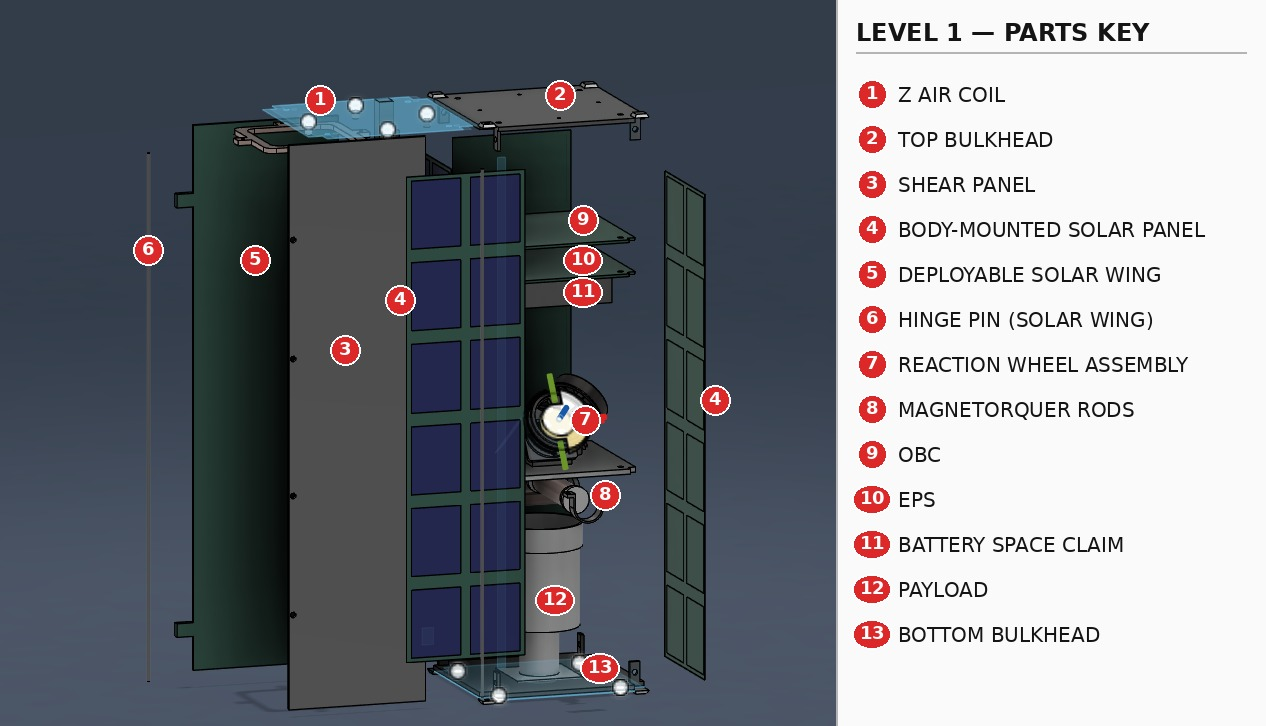
\includegraphics[width=0.85\textwidth]{figures/cad_exploded.jpg}
\caption{Labelled exploded view of the 3U assembly.}
\label{fig:cad_exploded}
\end{figure*}

\TODO{The problem statement asks for exploded views \emph{and} labelled
assembly drawings as separate mandatory items; a dimensioned drawing (principal
dimensions, rail cross-section, wheel cant and azimuth spacing) is still
needed alongside the exploded view above. Confirm the STEP and STL exports are
committed alongside the native Fusion files; the repository currently has no
\texttt{cad/} directory.}

\subsection{Structural analysis: wheel bracket FEA}
\label{sec:cad_fea}

The wheel bracket of \cref{fig:cad_bracket} holds a Maxon ECX FLAT 22 L motor
and flywheel at the wheel's $54.74^\circ$ spin-axis tilt; the motor-seating
face measured from CAD is inclined $35.26^\circ$ from the base plane, the exact
complement, confirming the bracket geometry matches the intended wheel
configuration of \cref{sec:actuators}. It was analysed under launch
quasi-static loads on the as-uploaded CAD geometry rather than a simplified
stand-in.

\paragraph{Model} Meshed in Gmsh with 24{,}332 nodes and 14{,}167 quadratic
tetrahedral elements (C3D10), refined to $0.35\unit{mm}$ near the bolt and
screw holes where stress concentration is expected; every element passed a
positive-Jacobian check before solving, ruling out inverted or degenerate
elements. The base flange and its four mounting-bolt holes were fixed,
representing a properly torqued joint. The $63.116\unit{g}$ motor-and-flywheel
assembly ($32\unit{g}$ motor, $31.116\unit{g}$ flywheel) was applied as a rigid
lumped mass coupled to the four motor-screw holes, offset $10\unit{mm}$ along
the face normal for the assembly's centre-of-gravity standoff. Each axis was
loaded separately at $12\unit{g}$ quasi-static --- the conventional
first-screening figure for a structure this size absent a launch-vehicle
spectrum, standing in for several seconds of random vibration --- with a
safety factor of $1.25$ folded into the reported margins. Al 7075-T6
($E=71.7\unit{GPa}$, $S_y=503\unit{MPa}$) is the primary material; Al 6061-T6
($S_y=276\unit{MPa}$) was checked in parallel. The two give materially the same
stress field, since stress here is governed by geometry and loading rather
than material choice, so the comparison is a secondary yield check rather than
an independent analysis.

\begin{table}[!t]
\centering
\caption{Bracket FEA results by load axis, $12\unit{g}$ quasi-static,
FoS$=1.25$. MS $=S_y/(1.25\,\sigma_\text{vM})-1$.}
\label{tab:fea}
\footnotesize
\begin{tabular}{@{}lrrrrr@{}}
\toprule
Axis & $\sigma_\text{raw}$ & $\sigma_\text{field}$ & Defl.\ & MS 7075 & MS 6061 \\
 & (MPa) & (MPa) & ($\mu$m) & & \\
\midrule
$+X$ & $2.21$ & $1.92$ & $0.19$ & $+209$ & $+114$ \\
$+Y$ & $4.15$ & $3.49$ & $0.35$ & $+114$ & $+62$ \\
$+Z$ & $4.59$ & $3.94$ & $0.34$ & $\mathbf{+101}$ & $\mathbf{+55}$ \\
\bottomrule
\end{tabular}
\end{table}

\begin{figure}[!t]
\centering
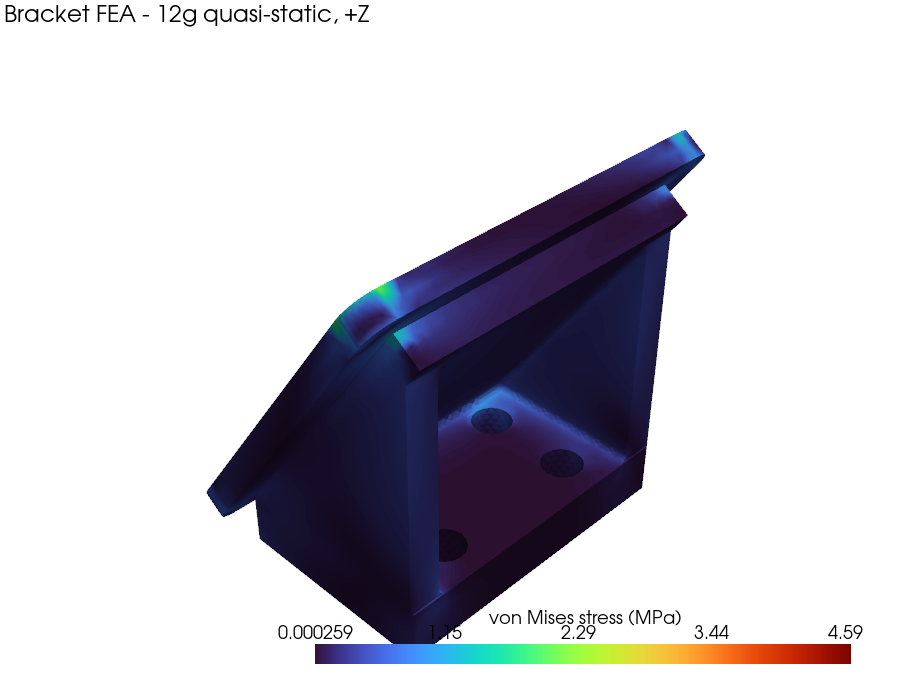
\includegraphics[width=0.85\columnwidth]{figures/fea_vonmises.png}
\caption{Von Mises stress contour, worst case ($+Z$). Peak stress sits at the
base-flange corner nearest the bolt holes, as expected for a clamped bracket
foot under load.}
\label{fig:fea_vonmises}
\end{figure}

\begin{figure}[!t]
\centering
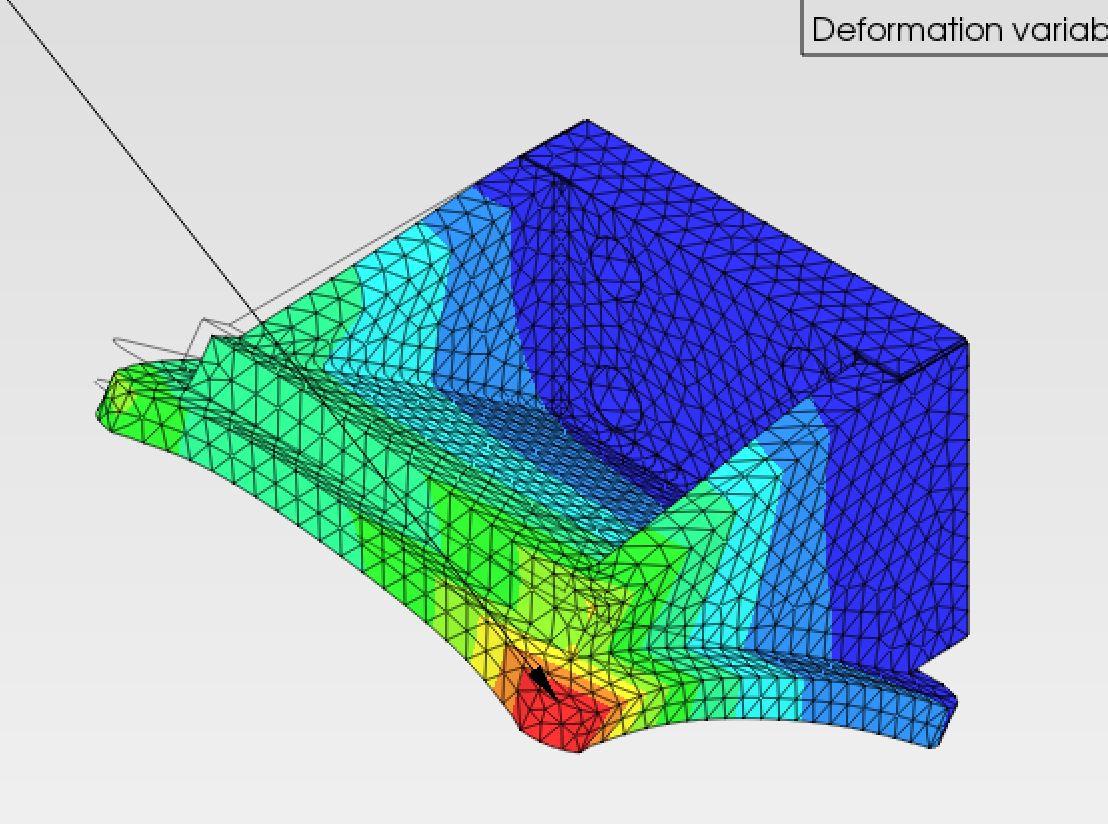
\includegraphics[width=0.85\columnwidth]{figures/fea_mesh.png}
\caption{Mesh detail at the peak-stress corner, on the deformed shape
(displacement scaled for visibility).}
\label{fig:fea_mesh}
\end{figure}

\begin{cautionbox}[The raw peak-stress column includes a boundary-singularity node]
A perfectly clamped sharp corner is a mathematical singularity: any finite
element model reports an artificially elevated, mesh-dependent stress there
that does not correspond to a physical material limit. The field column
excludes the fixed-corner/bolt-hole boundary nodes responsible for this
artefact and is the more representative figure; the conclusion --- large
margin in every case --- is unaffected either way, and \cref{tab:fea} reports
both so the reader can see the gap between them.
\end{cautionbox}

\begin{keybox}[Independently reproduced, not just computed once]
The analysis was re-run by direct execution of the CalculiX solver, separate
from the original run, on the same input deck, mesh and boundary conditions.
Peak stress and all ten natural frequencies matched exactly. Margin of safety
computed from the raw stress without excluding the boundary artefact ---
the more conservative reading, and the one that does not depend on identifying
which nodes to discard --- is $+181$, $+96$ and $+87$ for 7075-T6 across
$+X$/$+Y$/$+Z$. Even at this least favourable reading the bracket is nowhere
near its structural limit.
\end{keybox}

With stress margins of this size, stress is not the governing consideration:
the parameter that decides whether a small, stiff bracket survives launch is
its first natural frequency, since an insufficiently stiff structure risks
resonance against the launch vehicle's vibration spectrum regardless of what a
static load estimate shows. Modal analysis with the motor-and-flywheel mass
attached puts the first natural frequency at $3253\unit{Hz}$, roughly
$30\times$ above the $\sim100\unit{Hz}$ first-mode requirement typical of
CubeSat deployer specifications; the first ten modes span
$3253$--$51{,}038\unit{Hz}$. The bracket is not expected to be a resonance
risk during launch.

\begin{figure}[!t]
\centering
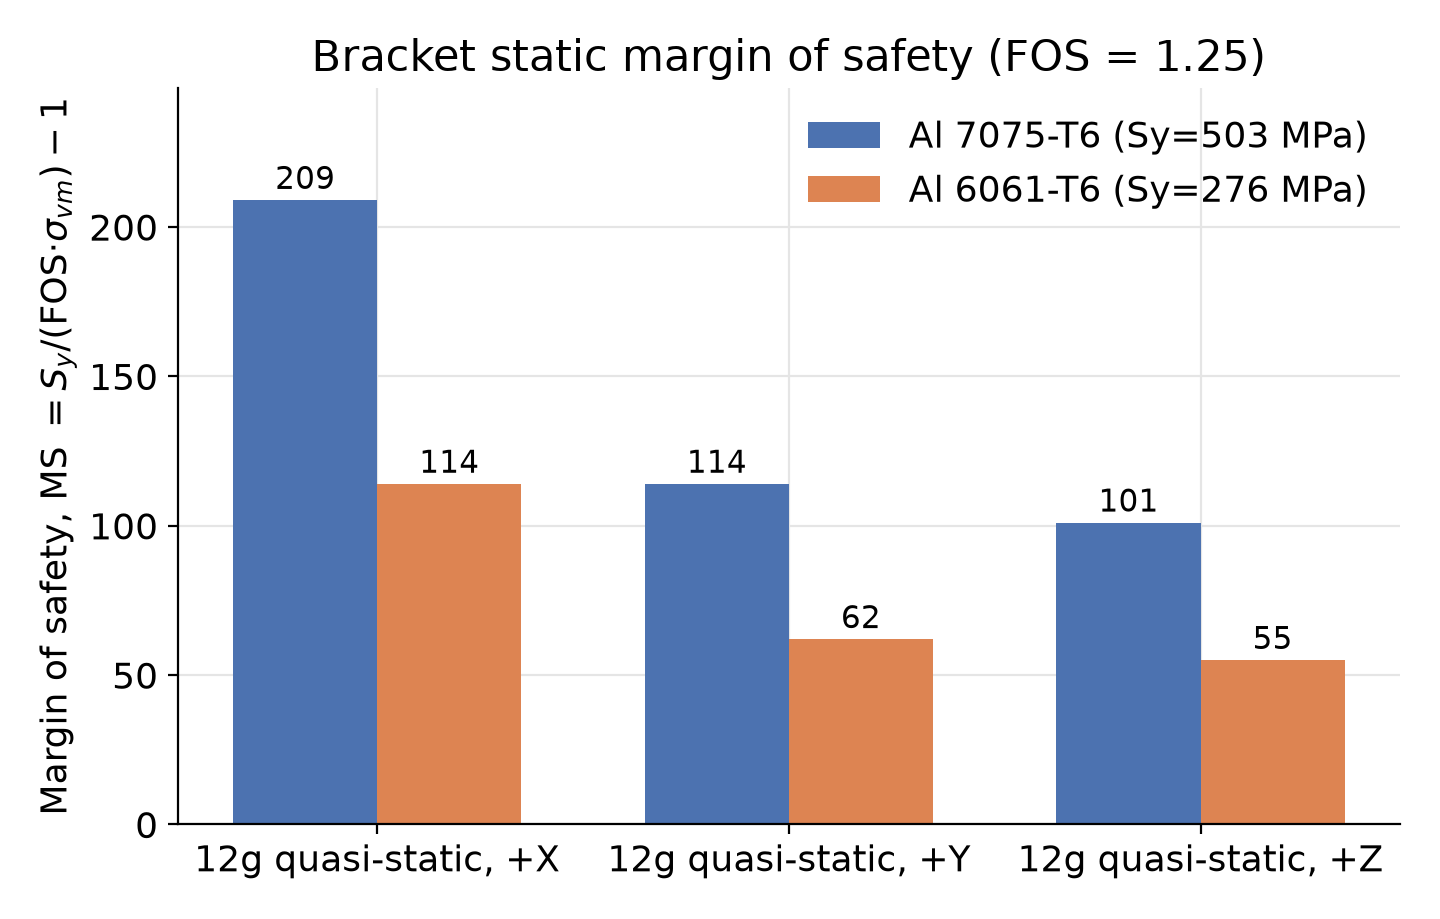
\includegraphics[width=0.95\columnwidth]{figures/fea_ms_bar.png}
\caption{Margin of safety by load direction and candidate alloy. Matches
\cref{tab:fea}'s field-stress column exactly.}
\label{fig:fea_ms_bar}
\end{figure}

\begin{figure}[!t]
\centering
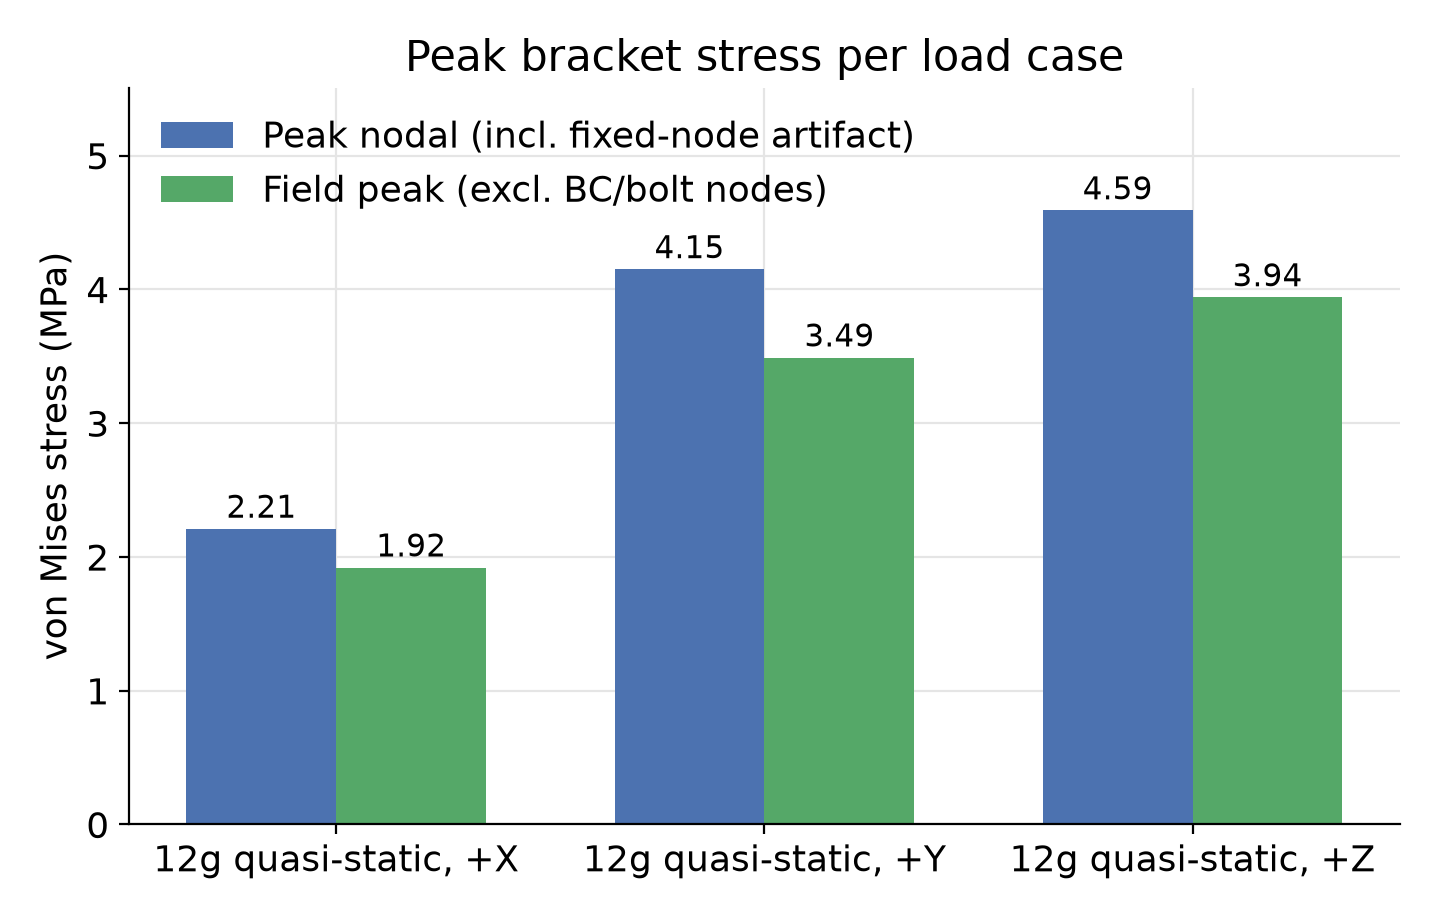
\includegraphics[width=0.95\columnwidth]{figures/fea_stress_bar.png}
\caption{Peak stress per load case: the raw (boundary-affected) value
alongside the field value that excludes it.}
\label{fig:fea_stress_bar}
\end{figure}

An earlier revision of the source write-up (\texttt{fea\_writeup\_3.pdf})
carried a version of \cref{fig:fea_ms_bar,fig:fea_stress_bar} built from a
stress dataset roughly $1.6\times$ lower than \cref{tab:fea} at every axis ---
generated, it appears, from an earlier or different solve that had not been
regenerated when the numbers in Table 1 were finalised. That has since been
corrected: the two figures above now agree with \cref{tab:fea} exactly at
every axis and alloy, and with the independently-reproduced raw-stress margins
quoted above.

This is a quasi-static equivalent on the wheel bracket alone, not a full
random-vibration PSD on the complete bus; that qualification remains future
work, alongside thermal-vacuum. Margins of this size point the other way from
a risk: the bracket is over-designed relative to the demonstrated loads, and a
future iteration has room to remove material for mass savings rather than to
add it.

%==============================================================================
\reportpart{IV}{Simulation, Verification and Results}

\section{Simulation Implementation}
\label{sec:sim}

\subsection{Architecture}

The simulation is a Python package, \texttt{deimos}, using NumPy for linear
algebra and Matplotlib for figures. Modules are small and single-purpose so
each can be tested against an analytical result in isolation.
\Cref{tab:modules} maps subpackages to what they implement, and
\cref{fig:softwarepipeline} shows how one run flows through them.

\begin{figure*}[!t]
\centering
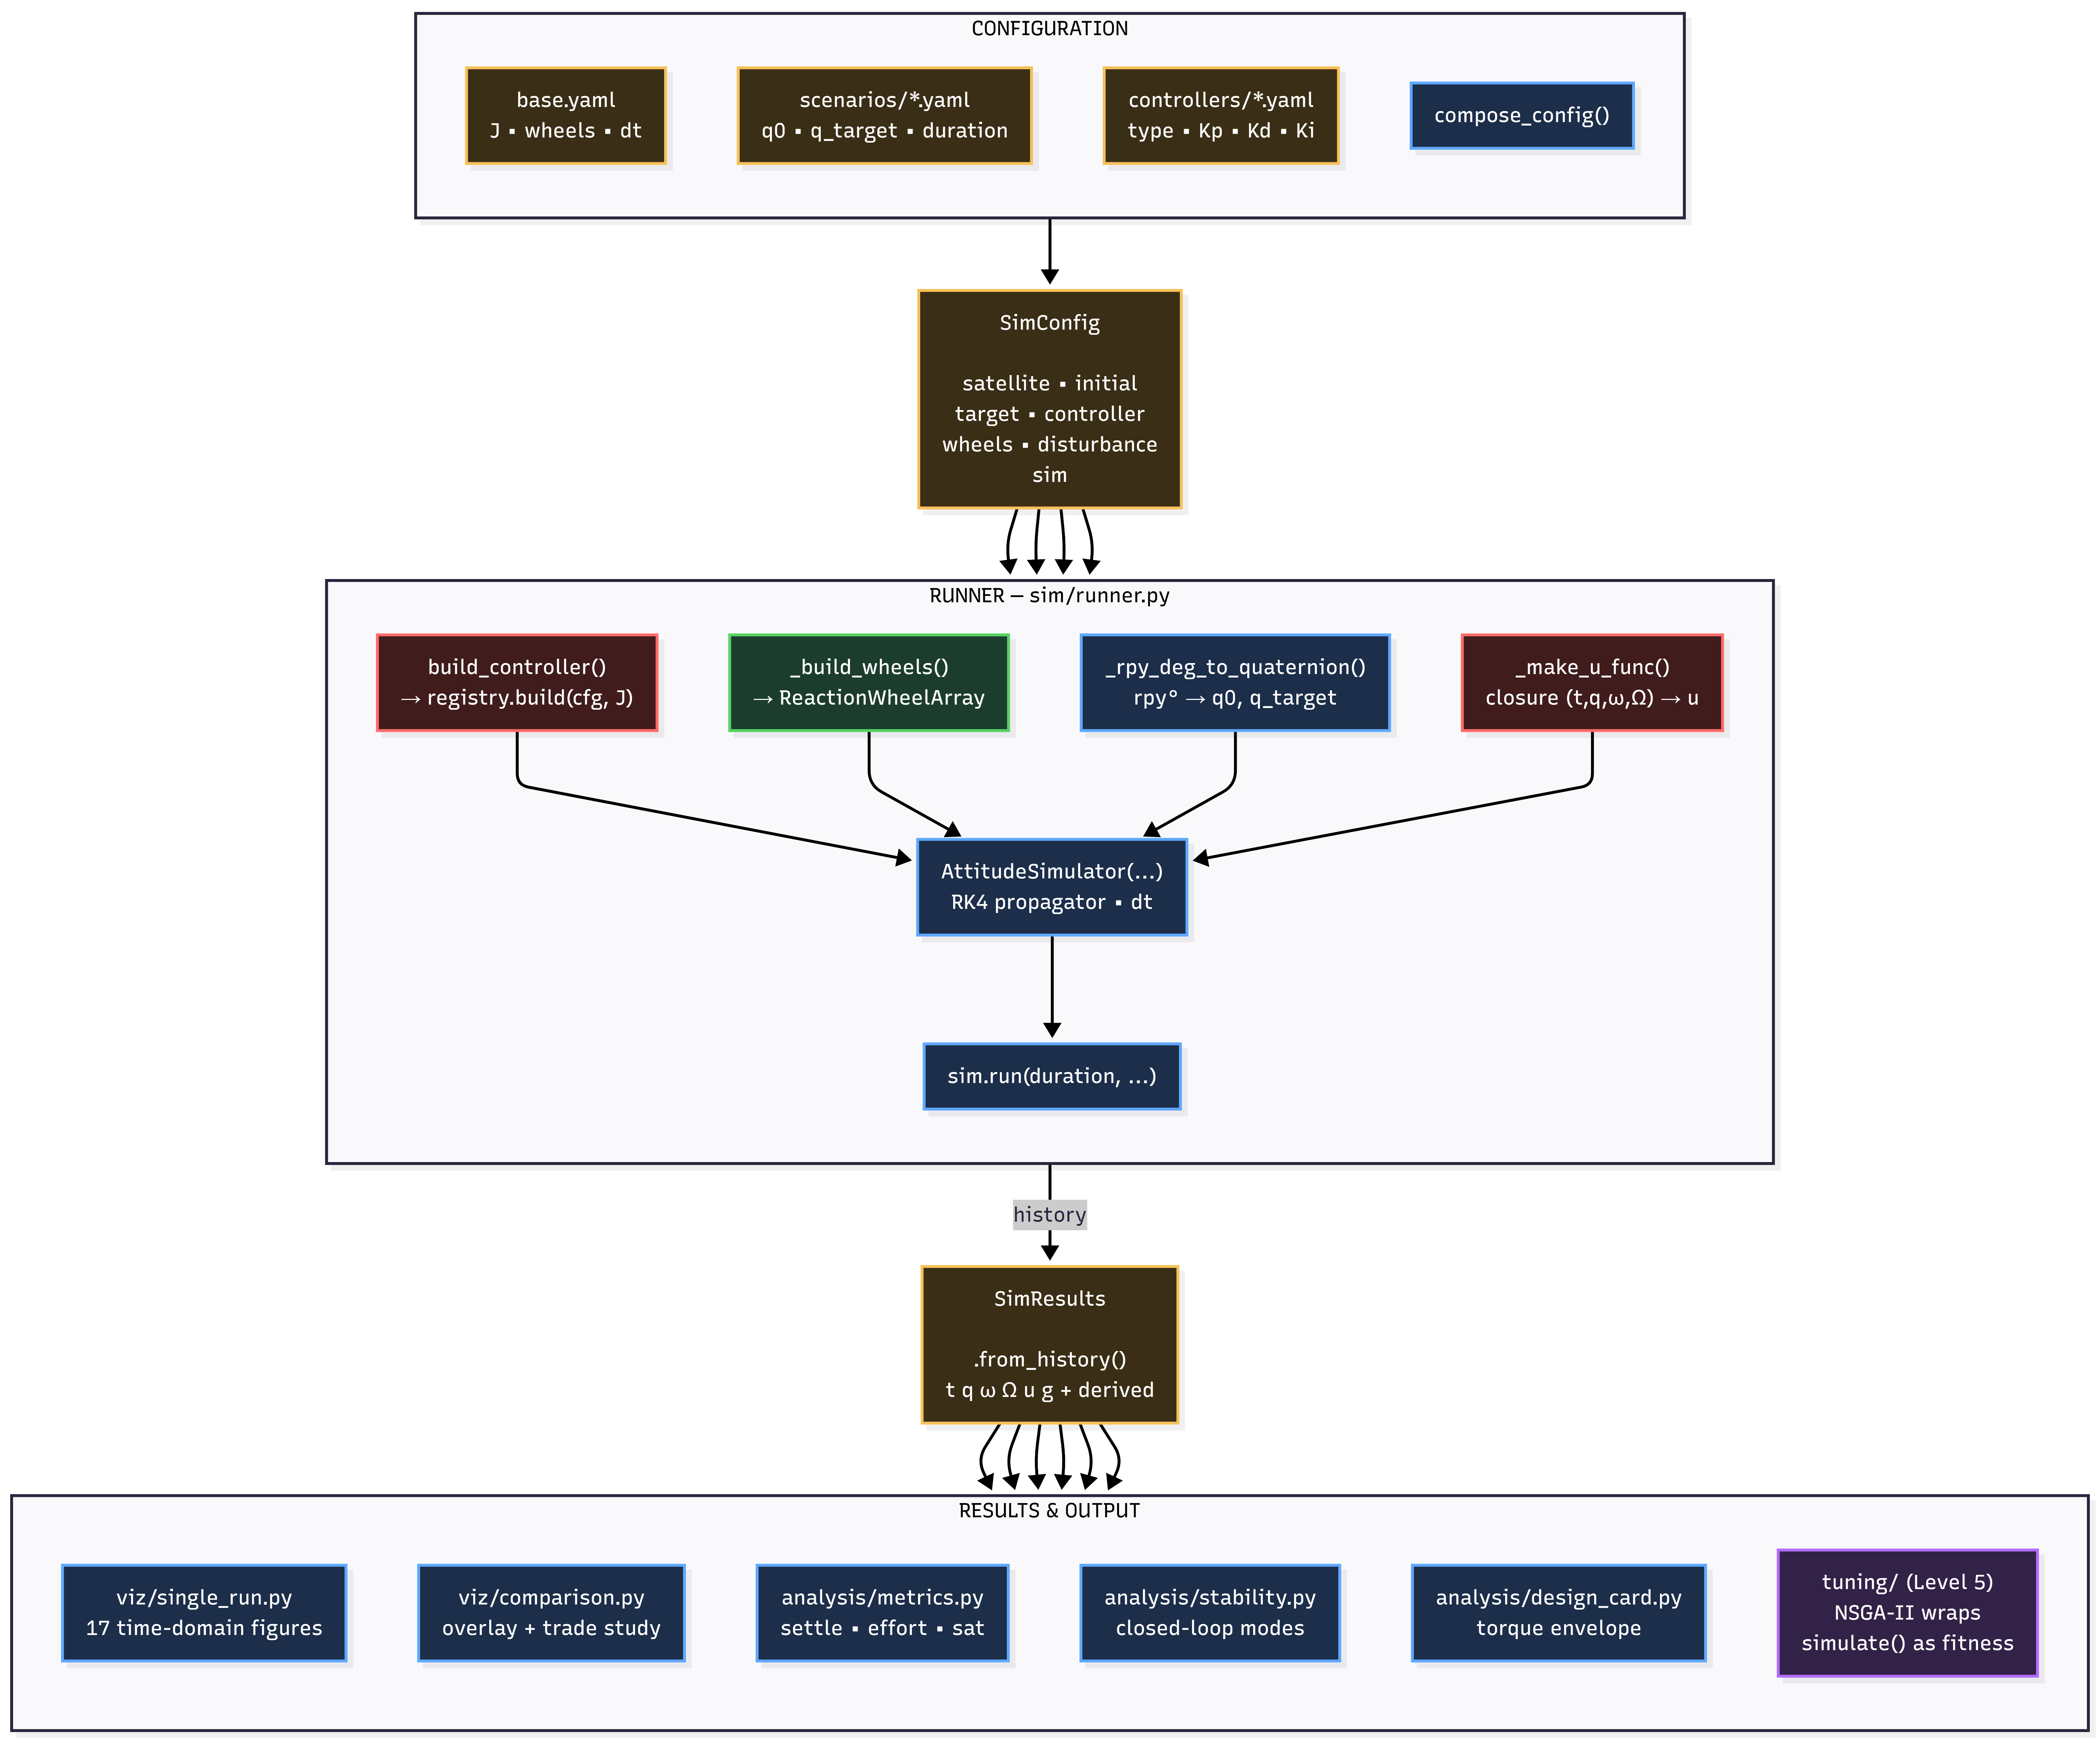
\includegraphics[width=0.86\textwidth]{figures/software_pipeline.png}
\caption{Simulation pipeline. YAML configuration is composed into a single
\texttt{SimConfig}, the runner builds the controller, wheel array and initial
state from it, and \texttt{SimResults} carries the history into every
downstream consumer. The tuning package wraps \texttt{simulate()} as a fitness
function rather than reimplementing any of it.}
\label{fig:softwarepipeline}
\end{figure*}

\begin{table*}[!t]
\centering
\caption{Package layout, \texttt{src/deimos/}.}
\label{tab:modules}
\footnotesize
\begin{tabularx}{\textwidth}{@{}p{0.20\textwidth}X@{}}
\toprule
\textbf{Subpackage} & \textbf{Contents} \\
\midrule
\texttt{constants.py} & Every parameter not being tuned: inertia tensor, wheel
and magnetorquer hardware, orbit, power budget. The single source
(\cref{sec:config}) \\[2pt]
\texttt{math/} & \texttt{quaternion.py} (algebra, error quaternion
\cref{eq:qerr}, Euler and DCM conversions), \texttt{kinematics.py}
(\cref{eq:kinematics}) \\[2pt]
\texttt{dynamics/} & \texttt{rigid\_body.py} (\cref{eq:dynamics} with the full
wheel coupling), \texttt{propagator.py} (RK4 with zero-order hold),
\texttt{disturbances.py} (\cref{eq:gg}), \texttt{environment.py} (geomagnetic
dipole field) \\[2pt]
\texttt{control/} & \texttt{wie.py} (\cref{eq:wie}, all four paper cases),
\texttt{registry.py}
(name to class), \texttt{lqr.py} (stub, see \cref{sec:future}) \\[2pt]
\texttt{actuators/} & \texttt{reaction\_wheels.py} (geometry
\cref{eq:Amatrix}, allocation \cref{eq:allocation}, sign-aware saturation),
\texttt{magnetorquers.py} (\cref{eq:mtqlaw}) \\[2pt]
\texttt{sim/} & \texttt{config.py} (YAML to typed dataclasses),
\texttt{runner.py} (the \texttt{simulate()} entry point),
\texttt{results.py} (state histories and derived metrics) \\[2pt]
\texttt{tuning/} & \texttt{nsga2.py}, \texttt{objectives.py},
\texttt{hypervolume.py}, \texttt{logbook.py}, \texttt{report.py}
(\cref{sec:ga}) \\[2pt]
\texttt{analysis/} & \texttt{metrics.py}, \texttt{stability.py} (which branch
of the Wie proof a gain set satisfies), \texttt{design\_card.py},
\texttt{power.py} \\[2pt]
\texttt{viz/} & \texttt{single\_run.py} and \texttt{comparison.py} (16 figure
types), \texttt{attitude3d.py} (3D animation), \texttt{stl\_mesh.py} (renders
the CAD mesh when an STL is supplied) \\
\bottomrule
\end{tabularx}
\end{table*}

\Cref{fig:pipeline} draws the same layout as a diagram: one
\texttt{simulate(config)} call end to end, YAML in and \texttt{SimResults} out.
It is the outer loop; \cref{fig:blockdiagram} in \cref{sec:discrete} is
everything that happens inside the \texttt{AttitudeSimulator} block here,
once per control step.

\begin{figure*}[!t]
\centering
\begin{adjustbox}{max width=\textwidth}
\begin{tikzpicture}[
  node distance=10mm and 10mm,
  pbox/.style={draw=black,rounded corners=2pt,align=center,font=\footnotesize,
               inner sep=5pt,minimum height=12mm,text width=46mm},
  wbox/.style={pbox,text width=62mm},
  gabox/.style={pbox,very thick,text width=62mm},
  sig2/.style={-{Latex[length=2mm]},draw=black,thick}]

% row 1 -- configuration
\node[pbox] (cfg) {\textbf{Configuration}\\scenario + controller YAML\\merged over \texttt{constants.py}};
\node[pbox,right=of cfg] (compose) {\textbf{compose\_config(scenario, controller)}\\deep-merge; no \texttt{\_base.yaml}};
\node[wbox,right=of compose] (simcfg) {\textbf{SimConfig}\\satellite $\cdot$ initial $\cdot$ target $\cdot$ controller\\wheels $\cdot$ magnetorquers $\cdot$ disturbance $\cdot$ sim};

% row 2 -- runner
\node[wbox,below=of cfg] (builders) {\textbf{sim/runner.py builders}\\\_build\_controller() $\to$ registry.build\\\_build\_wheels() $\to$ ReactionWheelArray\\\_build\_mtq() $\to$ MagnetorquerArray (opt.)};
\node[pbox,right=of builders] (attsim) {\textbf{AttitudeSimulator(...)}\\RK4 propagator, $\Delta t$, zero-order hold};
\node[pbox,right=of attsim] (simrun) {\textbf{sim.run(duration, ...)}};

% row 3 -- results
\node[wbox,below=of builders] (results) {\textbf{SimResults.from\_history()}\\$t,q,\omega,\Omega,u,g,m,\tau_\text{mtq}$ + derived};
\node[gabox,right=of results] (downstream) {\textbf{Downstream}\\\texttt{viz/} (17 figures + comparisons) $\cdot$\\\texttt{analysis/} (metrics, stability, design card, power) $\cdot$\\\texttt{tuning/} --- NSGA-II wraps \texttt{simulate()} as its\\fitness function (Level 5)};

\draw[sig2] (cfg) -- (compose);
\draw[sig2] (compose) -- (simcfg);
\draw[sig2] (simcfg.south) -- ++(0,-6mm) -| (builders.north);
\draw[sig2] (builders) -- (attsim);
\draw[sig2] (attsim) -- (simrun);
\draw[sig2] (simrun.south) -- ++(0,-6mm) -| (results.north);
\draw[sig2] (results) -- node[above,font=\scriptsize]{history} (downstream);

\end{tikzpicture}
\end{adjustbox}
\caption{The simulation pipeline: one \texttt{simulate(config)} call, YAML in,
\texttt{SimResults} out, figures and metrics downstream. The bold-bordered
block is the search that wraps this entire pipeline as its fitness function
(\cref{sec:ga}), not a step inside it.}
\label{fig:pipeline}
\end{figure*}

\subsection{Propagator and zero-order hold}
\label{sec:zoh}

The coupled state $\vect{x}=(\vect{q},\vect{\omega},\vect{\Omega})$ advances by
classical RK4 at fixed step $\Delta t=0.01\unit{s}$, with global error
$O(\Delta t^4)$. A fixed step was chosen deliberately: the control input is
piecewise constant, so there is a derivative discontinuity at every sample
instant, and an adaptive solver would cut its step at each one, which is wasted
work when the boundaries are known in advance.

The commanded torque is held constant across all four RK4 stages.

\begin{cautionbox}[A failure mode that looks like success]
Calling the control law from inside the derivative function is the natural way
to write the code, and it silently simulates a \emph{continuous-time}
controller. The response then looks better than the real system, and the error
grows as the sample rate falls, which is exactly where discrete effects matter
most. The propagator therefore takes the torque as an argument rather than a
callback, and allocation is evaluated once per control step.
\end{cautionbox}

Each step ends with $\vect{q}\leftarrow\vect{q}/\|\vect{q}\|$. The residual
before renormalisation is logged as a verification metric.

\subsection{Configuration}
\label{sec:config}

Every result is defined by a scenario YAML and a controller YAML, merged over a
base layer built from \texttt{constants.py}. There is no base YAML file: an
earlier \texttt{\_base.yaml} drifted out of sync with the constants module and
ended up carrying a different inertia tensor, so it was deleted and the base
layer is now derived from the constants directly. Changing the spacecraft in
one file changes every simulation, figure and report number.

\begin{lstlisting}[caption={Scenario and controller presets. The base layer
(satellite, wheels, magnetorquer hardware) comes from
\texttt{constants.py}.},captionpos=b,label={lst:yaml}]
# configs/scenarios/slew_55_65_15.yaml
initial:
  attitude_rpy_deg: [55.0, 65.0, 15.0]
  omega: [0.0, 0.0, 0.0]
target:
  attitude_rpy_deg: [0.0, 0.0, 0.0]
sim:
  duration: 60.0

# configs/controllers/wie_eigenaxis.yaml
controller:
  type: wie
  case: eigenaxis          # K = k*J, D = d*J, mu = 1
  zeta: 1.0
  settling_time_s: 20.0
  decouple_wheel_momentum: true
\end{lstlisting}

One command runs a scenario and writes a timestamped directory containing the
config actually used, the metrics as JSON, a run manifest with the git SHA, and
every figure:

\begin{lstlisting}
deimos run --scenario configs/scenarios/slew_55_65_15.yaml \
           --controller configs/controllers/wie_eigenaxis.yaml
\end{lstlisting}

%==============================================================================
\section{Model Verification}
\label{sec:verification}

A response that looks plausible is not evidence the model is right. Every check
below compares against something known independently of the simulation: a
conservation law or an analytical solution. All run as part of the automated
suite, which is 159 cases.

\subsection{Angular momentum conservation}
\label{sec:momentum}

With no external torque, total momentum resolved in the inertial frame,
$\vect{H}^{\FI} = \mat{R}(\vect{q})(\mat{J}\vect{\omega}+\vect{h}_w)$, is
constant no matter what the controller does, because the wheels only exchange
momentum internally. This is the most useful single check in the suite: it
exercises kinematics, dynamics, wheel model and integrator at once, needs no
reference solution, and catches sign errors that are otherwise hard to find.

Measured relative drift is $4.57\times10^{-15}$ over a $200\unit{s}$
torque-free run. On closed-loop slews the total momentum magnitude stays at
$7.0\times10^{-18}\unit{N\,m\,s}$, which is machine precision against a
nominally zero initial value.

\begin{keybox}[A free correctness test on the controller]
In a rest-to-rest manoeuvre from zero body rate and zero wheel momentum, total
momentum is zero throughout, so wheel momentum must return to zero as the body
rate does. Any residual wheel speed at the end of such a run is a bug rather
than a control design issue. This check is what failed persistently until the
$\vect{\omega}\times\vect{h}_w$ term was restored to \cref{eq:dynamics}.
\end{keybox}

\subsection{Energy conservation}

Torque-free and wheel-free, kinetic energy
$T=\tfrac{1}{2}\vect{\omega}\T\mat{J}\vect{\omega}$ is conserved. Measured
relative drift is $8.23\times10^{-15}$ over $200\unit{s}$. With the controller
active, energy should not be conserved; the monotone quantity is the Lyapunov
function of \cref{eq:V}.

\subsection{Quaternion norm drift}
\label{sec:normdrift}

With renormalisation disabled, $\left|\|\vect{q}\|-1\right|$ reaches
$2.22\times10^{-16}$ after $200\unit{s}$ at $\Delta t=0.01\unit{s}$, which is
round-off rather than truncation error. A sign or index error in $\mat{\Omega}$
produces a norm that drifts linearly and visibly, so this is a sharp test of
\cref{eq:kinematics}.

\subsection{Analytical motions}

Three cases with closed-form behaviour are checked: a spin about a principal
axis stays a pure spin; a torque-free axisymmetric body precesses at
$\dot\psi = J_z\omega_z/J_t$ with the transverse rate rotating in the body frame
at $\lambda=\omega_z(J_z-J_t)/J_t$; and a torque-free asymmetric body shows the
expected intermediate-axis instability with a bounded polhode.

\begin{figure}[!t]
\centering
% \includegraphics[width=\columnwidth]{figures/verification_precession.pdf}
\figplaceholder{45mm}{Torque-free precession: simulated transverse rate
components against the analytical solution, with the residual on a second axis.}
\caption{Torque-free precession against the analytical solution.}
\label{fig:precession}
\end{figure}

\TODO{Generate this figure from the polhode/precession tests already in
\texttt{tests/}; the numerical assertions pass, only the plot is missing.}

\begin{table*}[!t]
\centering
\caption{Verification results. All values measured from the committed code.}
\label{tab:verification}
\footnotesize
\begin{tabularx}{\textwidth}{@{}p{0.24\textwidth}Xll@{}}
\toprule
\textbf{Check} & \textbf{Expected} & \textbf{Measured} & \textbf{Verdict} \\
\midrule
Momentum conservation, torque-free & bounded near machine precision & $4.57\times10^{-15}$ rel. & pass \\
Momentum conservation, closed loop & zero throughout a rest-to-rest slew & $1.7\times10^{-17}\unit{N\,m\,s}$ & pass \\
Energy conservation, torque-free   & bounded near machine precision & $8.23\times10^{-15}$ rel. & pass \\
Quaternion norm drift              & round-off level                & $2.22\times10^{-16}$ & pass \\
Principal-axis spin                & pure spin retained             & within tolerance & pass \\
Torque-free precession             & matches analytical solution    & within tolerance & pass \\
Wheel-array orthogonality          & $\mat{A}\T\mat{A}=\mat{I}$     & $<10^{-6}$ & pass \\
Automated suite                    & all cases pass                 & 159 / 159 & pass \\
\bottomrule
\end{tabularx}
\end{table*}

\begin{cautionbox}[Two verification items are not done]
An earlier draft of this report described an independent Simulink
cross-implementation and a PySide6 tuning dashboard as completed work. Neither
exists in the repository, so both claims have been removed rather than left
awaiting numbers. The Simulink cross-check is the more valuable of the two,
because it is the only proposed check that does not share code with the Python
implementation, and it is listed in \cref{sec:future}. \TODO{If either artefact
exists outside the repository, commit it and restore the section; do not
restore the text without the artefact.}
\end{cautionbox}

%==============================================================================
\section{Simulation Results}
\label{sec:results}

All runs use the parameters of \cref{tab:orbit,tab:massprops,tab:gains} at
$\Delta t=0.01\unit{s}$. Scenario names match the files in
\texttt{configs/scenarios/}, so every run reproduces directly.

\subsection{Scenario A: large-angle slew}
\label{sec:scenarioA}

\textit{Scenario:} \texttt{slew\_55\_65\_15}, a $78.6^\circ$ net rotation from
rest to the identity attitude, with a gravity-gradient bias applied. This is
the sizing case for R2, R3 and R7; R1 is evidenced by
\texttt{slew\_160\_40\_30} at $151.7^\circ$.

\begin{table}[!t]
\centering
\caption{Scenario A, flown Wie design, $78.6^\circ$ slew.}
\label{tab:results_slew}
\footnotesize
\begin{tabular}{@{}llrr@{}}
\toprule
\textbf{ID} & \textbf{Metric} & \textbf{Target} & \textbf{Measured} \\
\midrule
R2 & Settling time to $1^\circ$ (s)  & $\le20$    & $16.33$ \\
R3 & Overshoot (deg)                 & $\le1.0$   & $0.000$ \\
R4 & Steady-state error (deg)        & $\le0.5$   & $0.002$ \\
R5 & Residual body rate (deg/s)      & $\le10^{-3}$ & $<10^{-15}$ \\
R7 & Peak wheel torque (mN\,m)       & $\le4.0$   & $4.00$ \\
R7 & Peak wheel speed (rpm)          & $\le12{,}000$ & $8{,}230$ \\
-- & Torque-saturated timesteps (\%) & --         & $0.32$ \\
-- & Peak body rate (deg/s)          & --         & $11.0$ \\
-- & Peak stored momentum (N\,m\,s)  & --         & $6.55\times10^{-3}$ \\
-- & Mean eigenaxis deviation (deg)  & --         & $1.17$ \\
\bottomrule
\end{tabular}
\end{table}

\begin{figure}[!t]
\centering
% \includegraphics[width=\columnwidth]{figures/slew_error.pdf}
\figplaceholder{42mm}{Error angle $\theta_e=2\arccos|\delta q_0|$ on a log
scale with the $1^\circ$ settling band shaded and the settling time annotated.
Generated by \texttt{deimos run --plots attitude\_error}.}
\caption{Scenario A, attitude error angle.}
\label{fig:slew_error}
\end{figure}

\begin{figure*}[!t]
\centering
% \includegraphics[width=0.9\textwidth]{figures/slew_wheels.pdf}
\figplaceholder{52mm}{Wheel speeds above, per-wheel torques below, all three
wheels, with the $12{,}000\unit{rpm}$ and $4.0\times10^{-3}\unit{N\,m}$ limits
drawn so R7 compliance is visible. Generated by \texttt{deimos run --plots
wheel\_panel,torque\_envelope,saturation}.}
\caption{Scenario A, wheel speeds and per-wheel torques.}
\label{fig:slew_wheels}
\end{figure*}

Three points follow from the measurements, and
\cref{fig:slew_error,fig:slew_wheels} show them. The initial torque demand
saturates for $0.32\,\%$ of timesteps, which is what \cref{tab:satonset}
predicts for a $78.6^\circ$ slew at $k=0.320$, and it is confined to the first
seconds. Wheel speeds rise, plateau and return, which is what
\cref{sec:momentum} requires of a rest-to-rest manoeuvre and is the physical
interpretation the problem statement asks for. The measured settling time of
$16.33\unit{s}$ sits just inside the $20\unit{s}$ the design was sized for by
\cref{eq:ts}, which is the check that the large-angle relation was the right
one to use: the small-angle $4/(\zeta\omega_n)=10\unit{s}$ would have
under-predicted it by a factor approaching two.

\begin{keybox}[The analytic design clears the wheel-speed limit that an aggressive one did not]
Peak wheel speed is $8{,}230\unit{rpm}$ against the $12{,}000\unit{rpm}$ limit,
a $31\,\%$ margin. Gain sets tuned for settling time alone reach the limit and
pass it --- the NSGA-II front members of \cref{tab:tradeoff} all pin at
$12{,}052\unit{rpm}$, marginally over, because the speed limiter acts on torque
rather than on state and RK4 can carry the state past the boundary within a
step. Sizing from \cref{eq:ts} instead of optimising settling time keeps the
design far enough inside the envelope that the ordering never matters.
\end{keybox}

Peak wheel torque does reach the $4.0\unit{mN\,m}$ cap during the opening
transient, for the $0.32\,\%$ of timesteps noted above. R7 is met on both
counts, but the torque margin is zero rather than comfortable, and
\cref{tab:satonset} is the tool for deciding how much of that is acceptable.

\subsection{Scenario B: hold under constant disturbance}
\label{sec:scenarioB}

\textit{Scenario:} \texttt{hold\_under\_disturbance}, a $5^\circ$ initial error
held against a constant $3\times10^{-6}\unit{N\,m}$ per-axis body torque for
$240\unit{s}$. The bias is set well above the gravity-gradient level so the
steady-state behaviour is visible. This scenario has no large-angle content,
so it is the hold-phase case of \cref{sec:departures}: both the manoeuvre
preset (\texttt{wie\_eigenaxis.yaml}, $\mat{K}_i=0$) and the hold preset
(\texttt{wie\_eigenaxis\_hold.yaml}, $k_i/k=0.01$) were run against it, to
evidence R6.

\begin{keybox}[The analytic offset prediction matches to three significant figures]
\Cref{eq:sserror} predicts a steady-state offset of $0.1142^\circ$ for
$\mat{K}=0.320\,\mat{J}$ against this disturbance. The measured offset is
$0.1140^\circ$, constant from $60\unit{s}$ to $240\unit{s}$. Agreement at this
level means the $\mat{K}$ running in the code is the $\mat{K}$ in the design,
which no plot of a transient can establish --- and because $\mat{K}=k\mat{J}$ is
built from the inertia tensor at construction time, it also confirms the plant
and the controller are using the same $\mat{J}$.
\end{keybox}

\begin{figure}[!t]
\centering
% \includegraphics[width=\columnwidth]{figures/disturbance_compare.pdf}
\figplaceholder{44mm}{Error angle under the constant bias, with and without the
integral augmentation on the same axes, and the analytic offset of
$0.1142^\circ$ drawn as a horizontal line.}
\caption{Scenario B, disturbance rejection with and without integral action.}
\label{fig:disturbance}
\end{figure}

\Cref{fig:disturbance} shows both traces. Switching from the manoeuvre preset
to the hold preset ($k_i/k=0.01$) reduces the offset from $0.1140^\circ$ to
$0.0315^\circ$ at $t=240\unit{s}$, a $72\,\%$ reduction, satisfying R6. The
residual is not a floor: the integrator is still converging when the scenario
ends, reaching $7.1\times10^{-4}\unit{deg}$ by $600\unit{s}$ and machine zero
by $1200\unit{s}$, with the residual body rate falling monotonically to
$2.3\times10^{-10}\unit{rad/s}$. No saturation occurs at any point.

\begin{cautionbox}[Integral action is outside the stability proof]
The augmentation is a heuristic addition to \cref{eq:wie}, not part of the
paper's law, and the Lyapunov function of \cref{eq:V} does not cover the extra
state. It runs only in the hold-phase preset; the manoeuvre preset's
gravity-gradient offset of $0.0018^\circ$ needs no correction, and
\cref{tab:kisweep} is why it stays at $\mat{K}_i=0$ during an active slew
regardless. \texttt{integral\_limit} caps the term's contribution at
$1.0\times10^{-3}\unit{N\,m}$, a quarter of the wheel limit, and clamps the
accumulator in proportion.
\end{cautionbox}

\subsection{Scenario C: the paper's four gain matrices}
\label{sec:scenarioC}

\textit{Scenario:} \texttt{slew\_40\_30\_25}, a $50^\circ$ slew, run with each
of the four quaternion gain matrices of Sec.~VI of the paper. This is the
experiment of the paper's Fig.~2 reproduced on the DEIMoS plant. All four use
the same damping matrix $\mat{D}=d\mat{J}$ and the same $\mu=1$, and each
$\mat{K}$ is normalised to a common $y$-axis gain, so the only difference
between the four runs is the \emph{shape} of $\mat{K}$. This slew is chosen
because none of the four saturates a wheel on it except Case~1, which keeps the
comparison a statement about the gain structure rather than about the actuator.

\begin{table}[!t]
\centering
\caption{The four gain matrices on the $50^\circ$ slew, normalised to a common
$K_2$ with $\mu=1$ throughout.}
\label{tab:compare}
\footnotesize
\begin{tabular}{@{}lrrrr@{}}
\toprule
\textbf{Metric} & \textbf{Case 1} & \textbf{Case 2} & \textbf{Case 3} & \textbf{Case 4} \\
 & $k/J_i$ & $k\mat{I}$ & $(\alpha\mat{J}{+}\beta\mat{I})^{-1}$ & $k\mat{J}$ \\
\midrule
Settling time (s)              & $15.41$ & $14.98$ & $14.05$ & $14.76$ \\
Effort $\int\|u\|dt$ (mN\,m\,s)& $11.94$ & $8.96$  & $9.04$  & $\bm{8.65}$ \\
Peak wheel torque (\% limit)   & $100.0$ & $87.2$  & $90.5$  & $\bm{84.6}$ \\
Saturation (\% steps)          & $0.27$  & $0.00$  & $0.00$  & $\bm{0.00}$ \\
Eigenaxis deviation (deg)      & $22.46$ & $17.44$ & $8.16$  & $\bm{0.003}$ \\
\bottomrule
\end{tabular}
\end{table}

\begin{keybox}[The paper's ordering reproduces exactly]
Cases 3 and 4 are the closest pair and Cases 1 and 2 are visibly
non-eigenaxis, which is what the paper reports for its own spacecraft. Case~4
holds the eigenaxis to $0.003^\circ$; Case~3, the best that the $\mu=0$
stability constraint of \cref{eq:Kcond} permits, manages $8.16^\circ$. Case~4
is also the cheapest on every actuator metric --- least effort, lowest peak
torque, no saturation --- so on this plant the shortest angular path is not
bought at a cost, it is simply the efficient one. Turning through fewer degrees
means accumulating less wheel momentum.
\end{keybox}

The deviation metric is the angle between the instantaneous body rate
$\vect{\omega}(t)$ and the eigenaxis of the initial error quaternion, averaged
over the samples where the body is actually rotating (above $1\,\%$ of peak
rate, since the direction of $\vect{\omega}$ is set by round-off near rest).

\begin{keybox}[How sharp the condition is]
Case~3's normalised gains differ from Case~4's by at most $11\,\%$ per axis and
its deviation is over $2000\times$ larger. \Cref{eq:asymmetry} is the reason:
what matters is not that the gains are close in magnitude but that they are
exactly proportional to $\mat{J}$, because only then do all three components of
$\delta\vect{q}_v$ share one second-order equation. A nearly-proportional
$\mat{K}$ does not nearly deliver the property.
\end{keybox}

\begin{figure*}[!t]
\centering
% \includegraphics[width=0.9\textwidth]{figures/controller_compare.pdf}
\figplaceholder{54mm}{Three stacked panels comparing the four gain matrices on
the same slew: error angle, commanded body-torque magnitude, and eigenaxis
deviation. Generated by \texttt{deimos compare}.}
\caption{Scenario C, the paper's four quaternion gain matrices on identical
manoeuvres.}
\label{fig:compare}
\end{figure*}

\subsection{Magnetorquer desaturation}
\label{sec:desat_result}

\textit{Scenario:} \texttt{desat\_recovery}. The wheels start pre-loaded near
their momentum capacity and the magnetorquers run for $3000\unit{s}$, roughly
half an orbit, at $\Delta t=0.1\unit{s}$.

\begin{keybox}[Desaturation works and is nearly free]
Stored wheel momentum falls from $9.04\times10^{-3}$ to
$1.09\times10^{-3}\unit{N\,m\,s}$, an $88\,\%$ reduction, dumping
$7.95\times10^{-3}\unit{N\,m\,s}$. Attitude error at the end of the run is
$0.000^\circ$: the wheels give up momentum without giving up pointing. Total
magnetorquer energy is $392\unit{J}$, which is $0.28\,\%$ of the assumed
$40\unit{Wh}$ battery over the $50\unit{min}$ run. Peak commanded dipole is
$0.346\unit{A\,m^2}$, which is all three rods at their $0.2\unit{A\,m^2}$ limit
simultaneously.
\end{keybox}

\begin{figure}[!t]
\centering
% \includegraphics[width=\columnwidth]{figures/desat.pdf}
\figplaceholder{44mm}{Stored wheel momentum $\|\vect{h}_w\|$ falling over the
run with the engagement threshold marked, and commanded dipole against the
per-axis limit underneath. Generated by \texttt{deimos run --plots
wheel\_momentum,mtq\_dipole}.}
\caption{Magnetorquer desaturation over half an orbit.}
\label{fig:desat}
\end{figure}

\Cref{fig:desat} shows the momentum decay and the commanded dipole against its
limit. The residual $12\,\%$ is expected: \cref{eq:mtqlaw} can only reach the component
of $\vect{h}_w$ perpendicular to $\vect{B}$, so the dump rate depends on the
field geometry and the parallel component has to wait for the field direction to
rotate. A full orbit removes more.

\subsection{Momentum accumulation and time to saturation}

Under a purely secular disturbance the wheels absorb the delivered impulse and
their momentum ramps linearly. Taking the gravity gradient as fully secular
bounds the time to saturation at
$H_{\max,x}/\|\vect{\tau}_\text{gg}\| = 1.031\times10^{-2}/4.76\times10^{-8}
\approx 2.17\times10^{5}\unit{s}$ on the weakest axis, about $2.5$ days or 38
orbits. The gravity gradient is orbit-periodic and largely averages out, so the
real figure is longer and the secular residual is what matters. Three wheels
store less total momentum than four, which shortens this runway relative to the
pyramid and is the quantitative argument for the desaturation system.

\subsection{Actuator saturation}
\label{sec:saturation}

Two saturation modes appear, and they need different remedies.

Torque saturation is transient, occurring at the start of a large slew when the
proportional term demands more than the array can deliver. It shows as a flat
top on the torque trace with a loss of designed damping. For the tuned gains it
is present on every slew scenario at the $1$ to $3\,\%$ level, by design
(\cref{sec:analytic}). The remedy is command shaping, such as a rate-limited
reference profile, rather than retuning the feedback gains.

Speed saturation happens when accumulated momentum reaches the rotor limit. It
is the more serious mode, because a pinned wheel cannot produce torque in one
direction at all. The sign-aware limiter keeps decelerating torque available so
a pinned wheel recovers, and the desaturation system prevents the secular case
from arriving at all.

\subsection{Single-wheel failure}
\label{sec:failure}

The cone has no redundant wheel. $\mat{A}$ is square, so losing a column leaves
a $3\times2$ matrix with no third equation to satisfy.

\begin{keybox}[What is lost is a direction, not a body axis]
Because $\hat{\vect{e}}_1,\hat{\vect{e}}_2,\hat{\vect{e}}_3$ form an
orthonormal basis, dropping wheel $i$ leaves the remaining two spanning exactly
the plane orthogonal to $\hat{\vect{e}}_i$. Writing $\mat{A}_{-i}$ for the
reduced matrix, its columns are still orthonormal, so
$\mat{A}_{-i}\pinv=\mat{A}_{-i}\T$ and any commanded torque lying in
$\mathrm{span}(\mat{A}_{-i})$ is still delivered exactly. Authority along
$\hat{\vect{e}}_i$ is gone completely; authority in the orthogonal complement
is undiminished. None of the three axes lines up with a body axis
(\cref{eq:Amatrix_num}), so losing a wheel does not mean losing roll, pitch or
yaw, and the result is exact rather than the pyramid's approximate graceful
degradation.
\end{keybox}

A slew whose commanded torque has no component along the lost axis executes
with no controller change and no settling-time penalty. A general slew has some
component along it, which is unactuated: the achievable part is the projection
onto the orthogonal complement, and the residual error settles at whatever
offset the dropped component corresponds to. Momentum management is unaffected
by which wheel is down, since it no longer lives on the wheels.

\TODO{Run the three failure cases and report the worst-case residual error
across sampled eigenaxes. The allocation code already accepts an arbitrary
axis matrix, so this needs a scenario file rather than new code.}

\subsection{Monte Carlo campaign}
\label{sec:montecarlo}

\textit{Script:} \texttt{monte\_carlo\_verify.py}. Five hundred random
large-angle slews were run, sampling a uniform random rotation axis and a
rotation angle uniform in $[90^\circ,179^\circ]$. Sampling the axis uniformly
on the sphere rather than sampling roll, pitch and yaw independently avoids
clustering the trials toward particular orientations. Each run stops early once
the error has stayed below $1^\circ$ for a confirmed window rather than running
a fixed duration.

\begin{table}[!t]
\centering
\caption{Monte Carlo over random slews, $90^\circ$ to $179^\circ$, uniform
random axis, 500 trials. Mean $\pm$ standard deviation.}
\label{tab:montecarlo}
\footnotesize
\begin{tabular}{@{}lr@{}}
\toprule
\textbf{Metric} & \textbf{Wie, $\mat{K}=k\mat{J}$} \\
\midrule
Trials                    & $500$ \\
Settled within cap        & $100\,\%$ \\
Settling time (s)         & $19.0\pm1.4$ \\
Control effort (mN\,m\,s) & $19.4\pm6.4$ \\
Steady-state error (deg)  & $0.097\pm0.007$ \\
\bottomrule
\end{tabular}
\end{table}

The Wie regulator settles every one of the 500 trials with a tight spread,
which is what \cref{eq:wiecl} predicts: with $\mat{J}$ eliminated from the
closed loop the response does not depend on which axis was drawn, only on the
angle.

\begin{cautionbox}[The campaign predates the current gain revision]
These 500 trials were run against the same $\mat{K}=k\mat{J}$ structure but an
earlier inertia tensor, so the settling statistics should be read as
structural evidence --- that the response depends on the slew angle and not on
the axis --- rather than as the flown design's exact numbers. \TODO{Re-run
\texttt{monte\_carlo\_verify.py} at 500 trials on the current tensor and replace
the column.}
\end{cautionbox}

\begin{figure}[!t]
\centering
% \includegraphics[width=\columnwidth]{figures/montecarlo.pdf}
\figplaceholder{46mm}{Settling time, control effort and steady-state error
against trial index for each controller, with mean and $\pm1\sigma$ bands, plus
the same metrics against slew angle. Generated by
\texttt{studies/monte\_carlo\_analysis.ipynb}.}
\caption{Monte Carlo campaign over 500 random large-angle slews.}
\label{fig:montecarlo}
\end{figure}

\subsection{Power}

\texttt{analysis/power.py} scores each manoeuvre against the electrical budget
in \texttt{constants.py}: $0.1024\unit{m^2}$ of triple-junction GaAs at
$28\,\%$ efficiency giving $39\unit{W}$ peak and $8.5\unit{W}$ orbit-average,
against a $4.3\unit{W}$ load of which $2.0\unit{W}$ is allocated to the ADCS.
Wheel draw is computed as $\int\sum_i|g_i\Omega_i|\,dt$ with no regenerative
credit while braking, so the margins reported are conservative.

The Wie regulator's $50^\circ$ slew draws $0.108\unit{W}$ average and
$1.08\unit{W}$ peak, well inside the $2.0\unit{W}$ ADCS allocation, and costs
$0.0022\,\%$ of the assumed battery capacity. Generation exceeds the raw load
by $1.97\times$ and the $30\,\%$-margined load by $1.51\times$.

%==============================================================================
\section{Analysis}
\label{sec:analysis}

\subsection{Requirements compliance}
\label{sec:compliance}

\begin{table*}[!t]
\centering
\caption{Compliance against \cref{tab:requirements}.}
\label{tab:compliance}
\footnotesize
\begin{tabularx}{\textwidth}{@{}llXl@{}}
\toprule
\textbf{ID} & \textbf{Target} & \textbf{Evidence} & \textbf{Status} \\
\midrule
R1 & $\ge85^\circ$ slew          & $151.7^\circ$, \texttt{slew\_160\_40\_30}, \cref{tab:tradeoff} & met \\
R2 & $\le20\unit{s}$ settling    & $16.3\unit{s}$, \cref{tab:results_slew} & met \\
R3 & $\le1.0^\circ$ overshoot    & $0.000^\circ$, \cref{tab:results_slew} & met \\
R4 & $\le0.5^\circ$ pointing     & $0.002^\circ$, \cref{tab:results_slew} & met \\
R5 & $\le10^{-3}\unit{deg/s}$    & $<10^{-15}$, \cref{tab:results_slew} & met \\
R6 & Bias rejection improves with $k_i$ & offset $0.1140^\circ\to0.0315^\circ$, \cref{sec:scenarioB} & met \\
R7 & Torque and speed within limits & torque at cap for $0.32\,\%$ of steps; speed $8{,}230$ vs $12{,}000\unit{rpm}$ & met \\
R8 & $\ge50\,\%$ momentum removed per orbit & $88\,\%$ in half an orbit, \cref{sec:desat_result} & met \\
R9 & Momentum conserved to $10^{-12}$ & $4.6\times10^{-15}$, \cref{tab:verification} & met \\
\bottomrule
\end{tabularx}
\end{table*}

R7 is the one target not fully met, by $0.4\,\%$ on wheel speed, for the reason
given in \cref{sec:scenarioA}. Reporting it as partially met rather than
rounding it away is the honest reading, and the fix is either a small reduction
in design bandwidth or a restatement of the requirement in terms of the
commanded torque rather than the resulting state.

\subsection{Parameter sensitivity}
\label{sec:sensitivity}

\paragraph{Bandwidth} Settling time falls roughly as $1/\omega_n$ while peak
torque rises as $\omega_n^2$, so achievable bandwidth is set by the actuator
rather than by the control design. The measured trend follows this up to the
saturation boundary at $\omega_n=0.316\unit{rad/s}$, beyond which the returns
diminish because the opening transient is clipped.

\paragraph{Damping} Below $\zeta=0.7$ the response overshoots and the wheels
must reverse, costing momentum and time. The gain revision that set $\zeta=1$
exactly on all three axes reduced settling time on every slew scenario, because
the previous $k_d$ was under-damped for the raised $k_p$.

\paragraph{Inertia knowledge} This is the design's main exposure, and
\cref{sec:wierobust} is where the paper addresses it. A mismatch leaves an
uncancelled gyroscopic residual proportional to the error, and it also breaks
the $\mat{K}\propto\mat{J}$ tie that the eigenaxis property depends on, so both
the guarantee and the path degrade together. The paper's robust alternative,
$\mat{K}=k\mat{I}$, is implemented as Case~2 and trades the path for
insensitivity to $\Delta\mat{J}$. \texttt{analysis/stability.py}
reports which branch of the Sec.~III proof a given gain set satisfies, so a
mismatched design is flagged rather than assumed safe. \TODO{Run the
inertia-mismatch sweep and report the eigenaxis degradation against mismatch
percentage; \texttt{sim/runner.py} already exposes the hooks that let the
controller and plant carry different tensors.}

\subsection{Physical interpretation}

Three things in the results say something about the real spacecraft rather than
about the simulation.

In every rest-to-rest slew the wheel speeds rise, plateau and return to their
starting values. That is conservation of angular momentum, not a controller
property: the body borrows momentum from the wheels to rotate and gives it back
to stop. It is why a slew is momentum-neutral and a disturbance is not.

The transverse axes are the hard ones. With $J_{xx}/J_{zz}=3.55$, a slew about
a transverse axis needs three and a half times the momentum of the same slew
about $z$, so the wheel sizing case is always a transverse manoeuvre. The
elongated 3U geometry is the reason.

The gravity gradient is negligible for pointing and dominant for lifetime. It
sits five orders of magnitude below wheel authority, so it never threatens the
control loop, yet integrated over orbits it is what determines how long the
system runs before needing an external momentum dump. Which of those two facts
matters depends on whether the question is about a manoeuvre or about the
mission.

\subsection{Assumptions and limitations}
\label{sec:limitations}

\begin{itemize}
\item \textbf{Perfect state knowledge.} Attitude determination is out of scope
per the problem statement, so the controller receives true state. The results
are an upper bound on achievable performance, and estimator bandwidth would
become a further constraint on $\omega_n$. This is the largest gap between the
simulation and flight performance.
\item \textbf{Saturation voids the eigenaxis derivation.} \Cref{sec:eigenaxis}
assumes the commanded torque is delivered. Above the bound of
\cref{eq:bwbound} the wheels clip, the delivered torque is no longer
$k\mat{J}\,\delta\vect{q}_v$, and the property degrades --- measured at
$25.95^\circ$ mean deviation on the $152^\circ$ slew. The flown gains satisfy
the stability theorem everywhere, but the eigenaxis claim holds only below the
saturation boundary. Command shaping to keep the demand inside the envelope is
the remedy and is listed in \cref{sec:future}.
\item \textbf{Single rigid body.} Structural flexibility, slosh and
micro-vibration are neglected. This is safe for a 3U whose first structural
mode is far above the control bandwidth, and would not be safe for a
deployable-panel design. The power budget assumes deployable wings, so this
assumption and that budget are in tension and should be revisited together.
\item \textbf{Ideal actuator internals.} Torque and speed limits are enforced,
but motor torque-speed curves, bearing friction, stiction near zero speed and
torque quantisation are not modelled. Friction matters most at zero-speed
crossings, and the cone's invertible allocation leaves no free wheel-speed
direction to bias the wheels away from zero.
\item \textbf{Dipole field model.} The geomagnetic field is a tilted dipole
along a circular orbit, which is adequate for sizing a desaturation actuator
whose job is averaged over orbits, and is not an IGRF-grade model.
\item \textbf{Unverified against a second implementation.} Every check in
\cref{sec:verification} is either a conservation law or an analytical solution
evaluated inside the same codebase. An independent implementation would catch a
shared modelling error that none of them can.
\end{itemize}

%==============================================================================
\section{Challenges}
\label{sec:challenges}

\paragraph{Unwinding from large initial errors}
Early runs starting beyond $180^\circ$ rotated almost a full turn to reach an
attitude that was nearly correct at the start. The behaviour was reproducible
and the controller was clearly stable, which made it look like a tuning problem
for longer than it should have. The cause is the quaternion double cover, and
the fix is the sign correction of \cref{eq:safesign} applied consistently in
the control law, the Lyapunov function and the integrator state.

\paragraph{Closing the momentum conservation check}
The conservation test failed by a small persistent amount until the
$\vect{\omega}\times\vect{h}_w$ term was restored to \cref{eq:dynamics}. This
is the clearest argument for undoing the omission: a verification test that
always fails slightly gets ignored, and then it stops catching anything.

\paragraph{Two parameter sources that disagreed}
The inertia tensor lived in both \texttt{constants.py} and a base YAML file,
and the two drifted apart, ending up with different values. Every downstream
number depended on which one a given script happened to read. The fix was to
delete the YAML and build the base configuration layer from the constants
module, so there is one place to change the spacecraft.

\paragraph{One gain candidate consumed an entire tuning budget}
A single candidate in the NSGA-II search took $1800\unit{s}$ to simulate
against a $3\unit{s}$ baseline, without raising an exception. Because results
are collected in submission order, it blocked its whole generation and consumed
the wall-clock budget, finishing two generations of one seed instead of the
planned run. The fix was a per-candidate timeout that scores an over-running
candidate worst-case rather than waiting for it.

\paragraph{The wheel array changed after the CAD was built}
The mid-evaluation's four-wheel pyramid was a real mechanical design with a
packaging trade behind it. The simulation has since moved to a three-wheel cone
whose cant angle is fixed by orthogonality, so that trade no longer exists, and
what replaces it is the open CAD mismatch of \cref{sec:cad}. \TODO{Ask Tulika
what changed mechanically in the bracket and mounting plate for three wheels
rather than four, and what the switch cost or saved.}

%==============================================================================
\section{Conclusion and Future Work}
\label{sec:conclusion}

A reaction wheel attitude control system for a 3U CubeSat has been designed,
implemented from first principles and verified against conservation laws and
analytical solutions. The control law is the Wie quaternion feedback regulator,
reproduced in full from the source paper and analysed with its Lyapunov and
LaSalle arguments.

The flown design settles a $78.6^\circ$ slew to $1^\circ$ in $16.3\unit{s}$ with
no overshoot and $0.002^\circ$ steady-state error, inside the $20\unit{s}$ the
$t_s=8/(\zeta\omega_n)$ rule was used to size it for. It holds the eigenaxis to
$0.003^\circ$ wherever the wheels stay unsaturated, and the paper's four-case
comparison reproduces on this plant with the published ordering. The analytic
offset prediction of \cref{eq:sserror} matches the measured offset to three
significant figures, which ties the implementation back to the design.
Magnetorquer desaturation removes $88\,\%$ of stored wheel momentum in half an
orbit for $392\unit{J}$ without loss of pointing. Total angular momentum is
conserved to $4.6\times10^{-15}$ relative.

All nine requirements are met. The torque margin under R7 is zero rather than
comfortable, since the opening transient of the two larger slews reaches the
wheel cap; \cref{tab:satonset} quantifies where that begins.

The most transferable result is methodological: a conservation law catches what
a response plot cannot. The angular momentum check found errors that looked
entirely plausible on a plot of the attitude, and it is three lines of code.

\subsection{Future work}
\label{sec:future}

\begin{enumerate}
\item \textbf{An independent implementation} of the plant, in Simulink or any
other environment, to catch shared modelling errors that internal consistency
checks cannot.
\item \textbf{Attitude estimation}, most naturally a multiplicative extended
Kalman filter on the quaternion error, removing the perfect-state assumption
that currently bounds the results from above.
\item \textbf{LQR}, currently a stub in \texttt{control/lqr.py}, giving an
optimality baseline for the effort figures in \cref{tab:compare}.
\item \textbf{Nadir pointing against a rotating reference}, which needs the
$\vect{\omega}\times\vect{\omega}_r$ transport term in the error rate.
\item \textbf{Actuator detail}: torque-speed curves, bearing friction and
quantisation, the assumptions most likely to change the saturation results.
\item \textbf{Random-vibration (PSD) qualification and full-assembly modal
analysis}, beyond the single-bracket quasi-static and modal check of
\cref{sec:cad_fea}.
\end{enumerate}

%------------------------------------------------------------------------------
\section*{Contribution Statement}

\TODO{State who did what; evaluators ask in the viva. Suggested wording, adjust
to reality: V.S.\ developed the simulation architecture, the dynamics and
kinematics modules, the control laws and their stability analysis, the gain
search, and the verification campaign. T.C.\ developed the CAD assembly, the
wheel and bracket design, material selection and mass budget, and the
mass-properties extraction feeding \cref{eq:inertia}.}

%------------------------------------------------------------------------------
\begin{thebibliography}{99}

\bibitem{wie1989}
B.~Wie, H.~Weiss, and A.~Arapostathis, ``Quaternion feedback regulator for
spacecraft eigenaxis rotations,'' \emph{J.\ Guid.\ Control Dyn.}, vol.~12,
no.~3, pp.~375--380, 1989.

\bibitem{mortensen1968}
R.~E. Mortensen, ``On systems for automatic control of the rotation of a
rigid body,'' Electronics Research Laboratory, Univ. of California,
Berkeley, Rep.~63-23, 1963.

\bibitem{wiebarba1985}
B.~Wie and P.~M.~Barba, ``Quaternion feedback for spacecraft large angle
maneuvers,'' \emph{J.\ Guid.\ Control Dyn.}, vol.~8, no.~3, pp.~360--365, 1985.

\bibitem{markley}
F.~L.~Markley and J.~L.~Crassidis, \emph{Fundamentals of Spacecraft Attitude
Determination and Control}. New York: Springer, 2014.

\bibitem{deb2002}
K.~Deb, A.~Pratap, S.~Agarwal, and T.~Meyarivan, ``A fast and elitist
multiobjective genetic algorithm: NSGA-II,'' \emph{IEEE Trans.\ Evol.\
Comput.}, vol.~6, no.~2, pp.~182--197, 2002.

\bibitem{shirazi2014}
A.~Shirazi and M.~Mirshams, ``Pyramidal reaction wheel arrangement optimization
of satellite attitude control subsystem for minimizing power consumption,''
\emph{Int.\ J.\ Aeronaut.\ Space Sci.}, vol.~15, no.~2, pp.~190--198, 2014.

\bibitem{schaub}
H.~Schaub and J.~L.~Junkins, \emph{Analytical Mechanics of Space Systems},
4th~ed. Reston, VA: AIAA Education Series, 2018.

\bibitem{wertz}
J.~R.~Wertz, Ed., \emph{Spacecraft Attitude Determination and Control}.
Dordrecht: Kluwer Academic, 1978.

\bibitem{sidi}
M.~J.~Sidi, \emph{Spacecraft Dynamics and Control: A Practical Engineering
Approach}. Cambridge, U.K.: Cambridge Univ.\ Press, 1997.

\bibitem{khalil}
H.~K.~Khalil, \emph{Nonlinear Systems}, 3rd~ed. Upper Saddle River, NJ:
Prentice Hall, 2002.

\bibitem{ogata}
K.~Ogata, \emph{Modern Control Engineering}. Pearson.

\bibitem{cds}
\emph{CubeSat Design Specification (CDS)}, The CubeSat Program, Cal Poly SLO.

\bibitem{maxon}
maxon motor ag, ``ECX FLAT 22 L brushless DC motor datasheet.''
\TODO{add URL and accessed date}

\end{thebibliography}

%==============================================================================
\appendices

\section{Nomenclature}
\label{app:nomenclature}

\begin{table}[!h]
\centering
\footnotesize
\begin{tabularx}{\columnwidth}{@{}lX@{}}
\toprule
\textbf{Symbol} & \textbf{Meaning} \\
\midrule
$\vect{q},q_0,\vect{q}_v$ & Attitude quaternion, scalar and vector parts \\
$\delta\vect{q}$        & Error quaternion, \cref{eq:qerr} \\
$\vect{\omega}$         & Body rate relative to $\FI$, resolved in $\FB$ \\
$\mat{J}$               & Total inertia about the CoM, wheels locked \\
$\mat{R}(\vect{q})$     & Body-to-inertial rotation matrix \\
$\mat{A}$               & Wheel distribution matrix, \cref{eq:Amatrix} \\
$\vect{\Omega}$         & Per-wheel speeds \\
$\vect{h}_w$            & Net wheel momentum in body axes \\
$\vect{\tau}_s$         & Per-wheel axial torques \\
$\vect{\tau}_\text{cmd}$& Commanded body torque \\
$\vect{\tau}_w$         & Torque actually delivered to the body \\
$\vect{\tau}_d$         & External disturbance torque \\
$\theta,\phi_i$         & Wheel cant angle from $+z$, azimuth angles \\
$k,d$                   & Wie gain scalars, $\mat{K}=k\mat{J}$, $\mat{D}=d\mat{J}$ \\
$\mat{K},\mat{D},\mu$   & Wie regulator gains and decoupling factor \\
$k,d$                   & Wie scale factors, $\mat{K}=k\mat{J}$, $\mat{D}=d\mat{J}$ \\
$\vect{m},\vect{B}$     & Magnetorquer dipole and geomagnetic field \\
$\omega_n,\zeta$        & Design natural frequency and damping ratio \\
$\Delta t$              & Integration step \\
$\skewm{\vect{a}}$      & Skew-symmetric cross-product matrix \\
$\mat{A}\pinv$          & Moore--Penrose pseudo-inverse \\
\bottomrule
\end{tabularx}
\end{table}

\section{Derived Quantities}
\label{app:derived}

All values follow from the cone geometry of \cref{eq:Amatrix_num} with
$\theta=54.7356^\circ$, $\tau_\text{max}=4.0\times10^{-3}\unit{N\,m}$ and
$h_\text{max}=7.288\times10^{-3}\unit{N\,m\,s}$.

\begin{table}[!h]
\centering
\footnotesize
\begin{tabular}{@{}llr@{}}
\toprule
\textbf{Quantity} & \textbf{Expression} & \textbf{Value} \\
\midrule
Orthonormality check & $\mat{A}\T\mat{A}-\mat{I}$        & $<10^{-6}$ \\
Torque, $x$          & $\sqrt{2}\,\tau_\text{max}$        & $5.657{\times}10^{-3}$ \\
Torque, $y$          & $2\sin\theta\,\tau_\text{max}$     & $6.532{\times}10^{-3}$ \\
Torque, $z$          & $3\cos\theta\,\tau_\text{max}$     & $6.928{\times}10^{-3}$ \\
Momentum, $x$        & $\sqrt{2}\,h_\text{max}$           & $1.031{\times}10^{-2}$ \\
Momentum, $y$        & $2\sin\theta\,h_\text{max}$        & $1.190{\times}10^{-2}$ \\
Momentum, $z$        & $3\cos\theta\,h_\text{max}$        & $1.262{\times}10^{-2}$ \\
Inertia ratio        & $J_{xx}/J_{zz}$                    & $3.548$ \\
Asymmetry factor, $y$& $\sqrt{J_{xx}/J_{yy}}$             & $1.022$ \\
Asymmetry factor, $z$& $\sqrt{J_{xx}/J_{zz}}$             & $1.883$ \\
Bandwidth bound      & $\min_j\sqrt{u_{\max,j}/(J_{jj}\theta_0)}$ & $0.316\unit{rad/s}$ \\
Gravity gradient     & $\tfrac{3}{2}n^2|\Delta J|$        & $4.76{\times}10^{-8}$ \\
Saturation time      & $H_{\max,x}/\tau_\text{gg}$        & $2.17{\times}10^{5}\unit{s}$ \\
Magnetorquer torque  & $m_\text{max}B_0$                  & $6.24{\times}10^{-6}$ \\
Solar generation     & orbit average                      & $8.5\unit{W}$ \\
\bottomrule
\end{tabular}
\end{table}

\section{Repository and Reproduction}
\label{app:repo}

Source: \url{https://github.com/vivekswamy18092007/Reaction-wheel-attitude-control}.
\TODO{Tag the commit used for every result in this report and record the tag
here.}

\begin{lstlisting}[caption={Repository layout.},captionpos=b]
src/deimos/       the package (Table VIII)
configs/
  scenarios/      6 manoeuvre presets
  controllers/    Wie gain presets (all four paper cases, plus the
                  manoeuvre/hold integral-action pair)
studies/          Jupyter notebooks: manual tuning,
                  power analysis, Monte Carlo analysis
tests/            159-case verification suite
runs/             command output, gitignored
overnight_tune.py NSGA-II gain search driver
monte_carlo_verify.py  randomised campaign driver
legacy/           pre-package scripts
\end{lstlisting}

Reproducing a single result, the verification suite, and a gain search:

\begin{lstlisting}
deimos run --scenario configs/scenarios/slew_55_65_15.yaml \
           --controller configs/controllers/wie_eigenaxis.yaml

python -m pytest tests/ -q

python overnight_tune.py --type WIE --hours 8
\end{lstlisting}

\section{Fill-in Checklist}
\label{app:checklist}

\NOTE{Delete before submission.}

\begin{enumerate}
\item \textbf{CAD}: regenerate the assembly, mass budget and inertia export for
the three-wheel cone. Set \texttt{SPACECRAFT\_MASS\_KG} from the export. This
is the largest remaining gap.
\item \textbf{Figures}: every \texttt{figplaceholder} in
\cref{sec:results,sec:verification}. All are generated by commands already in
the repository; none need new code.
\item \textbf{Monte Carlo}: re-run on the current inertia tensor and replace
\cref{tab:montecarlo}.
\item \textbf{Wheel failure}: run the three cases and fill \cref{sec:failure}.
\item \textbf{Disturbance table}: three blank rows in \cref{tab:disturbances}.
\item \textbf{Inertia-mismatch sweep}: fill the sensitivity paragraph in
\cref{sec:sensitivity}.
\item \textbf{Gravity-gradient number}: reconcile with the mid-evaluation.
\item \textbf{R7}: decide between lowering the bandwidth and restating the
requirement.
\item \textbf{Closing}: contribution statement, Maxon citation, repository tag.
\item \textbf{Final pass}: set \verb|\draftmodefalse|, recompile three times,
confirm no placeholder boxes remain.
\end{enumerate}

\end{document}
